% LaTeX source for book ``代数学方法'' in Chinese
% Copyright 2018  李文威 (Wen-Wei Li).
% Permission is granted to copy, distribute and/or modify this
% document under the terms of the Creative Commons
% Attribution 4.0 International (CC BY 4.0)
% http://creativecommons.org/licenses/by/4.0/

% To be included
\chapter{群论}
群是代数学中最基本的结构之一. 本章涉及的内容大致有两类:
\begin{compactenum}
	\item 形式构造, 包括幺半群和群的基本定义, 群作用, 直积, 自由群等概念, 这也是研究其它代数结构的基石.
	\item 群本身的具体性质, 主要是组合面向, 包括有限群的 Sylow 三定理, 对称群和辫群的展示等. 这部分较富技巧性, 是群论引人入胜之处.
\end{compactenum}
我们力求做到两者的交错搭配. 对于群论的基本概念, 本书不予连篇累牍的辨析, 但在形式性质及一些初等教材遗漏的重要构造 (如自由群, 完备化等) 方面则力求详备, 这也是为后续章节作铺垫. 至于群论的具体部分, 对称群可谓是群论和表示理论的思想泉源之一, 相关的 \S\ref{sec:symmetric-group} 是对此前理论的一次总操练. 有限生成交换群的分类是群论的另一个重要结果, 本书将其纳入模论处理, 见 \S\ref{sec:PID-module}.

尽管本章在逻辑上几乎是自足的, 我们期望读者对群有些许的基本认知. 此后凡论及群, 幺半群或其它代数结构组成的范畴时, 若无另外申明, 则一律沿用关于 Grothendieck 宇宙的约定 \ref{con:U-small}, 默认这些对象都是``小''的.

\begin{wenxintishi}
	从 \S\ref{sec:group-and-monoid} 到 \S\ref{sec:group-action} 的内容属于群论的基础知识, 本章只是采取了一个稍广泛的框架. 随后的内容相较之下需要一定的技术, 然而也同样初等. \S\ref{sec:free-group} 讨论的自由群无论怎么构造都难免琐碎, 本章从自由幺半群和融合积切入, 论证稍长但得到的结果更多, 实用上也是必要的.

	如前所述, 对称群 (\S\ref{sec:symmetric-group}) 是一类不得不谈的重要实例. 极限和完备化 (\S\ref{sec:group-limit}) 涉及一些点集拓扑的语言, 对以后要陈述的无穷 Galois 理论不可或缺, 更是从事进一步研究的必备素养.

	本章的缺憾之一在于未探讨正多面体的旋转对称群, 这是几何直观与群论技巧的优美嵌合; 譬如正十二面体和正二十面体的群相同, 是 $60$ 阶单群, 从它到交错群 $\mathfrak{A}_5$ 的同构可用几何语言表述. 了解经典内容大有益处, 建议读者参阅相关教材如 \cite[Chapter 8]{Har00}.
\end{wenxintishi}

\section{半群, 幺半群与群}\label{sec:group-and-monoid}
本节借鉴 Bourbaki \cite{Bou-Alg1} 定义代数结构的进路, 思路是从带有\emph{二元运算}的集合出发. 非空集合 $S$ 上的二元运算意谓一个映射 $S \times S \to S$, 一般用乘法记号写为 $(x, y) \mapsto x \cdot y$, 或索性简写为 $xy$; 二元运算可视作 $S$ 上的某种乘法. 反复操作可以得到形如 $x(yz)$, $(wx)(yz)$ 等等的表达式, 括号在此表示元素相乘的先后顺序. 如不致混淆, 我们经常略去结构 $(S, \cdot)$ 中的二元运算, 径以 $S$ 概括. Bourbaki 为这种混沌未开的结构起了个贴切的名字, 唤作``岩浆'' (法文: le magma). \index{eryuanyunsuan@二元运算 (binary operation)}

首先收集关于 $(S, \cdot)$ 的一些初步概念.
\begin{itemize}
	\item 在 $S$ 上定义新的二元运算 $\star$ 使得 $x \star y = y \cdot x$, 得到的新结构 $(S, \star)$ 记作 $S^\text{op}$, 称为 $S$ 的相反结构.
	\item 若对所有 $x, y \in S$ 都有等式 $xy=yx$, 则称 $S$ 满足\emph{交换律}, 或称 $S$ 是交换的; 这等价于 $S = S^\text{op}$.\index{jiaohuan@交换}
	\item 若对所有 $x, y, z \in S$ 都有等式 $(xy)z=x(yz)$, 则称 $S$ 满足\emph{结合律}.
	\item 设 $u \in S$, 若相应的从 $S$ 到 $S$ 的\emph{左乘}映射 $x \mapsto ux$ 是单射, 则称 $u$ 满足左消去律; 若\emph{右乘}映射 $x \mapsto xu$ 是单射, 则称 $u$ 满足右消去律.
	\item 若 $A, B$ 为 $S$ 的子集, 定义
		\[ A B := \{ab : a \in A, \; b \in B \} \subset S; \]
		若 $A$ 或 $B$ 是独点集 $\{x\}$, 则 $AB$ 相应地写作 $xB$ 或 $Ax$; 在结合律的前提下还可以无歧义地定义子集 $ABC$, $ABCD$,......
	\item 若 $S$ 的子集 $A$ 满足 $A A \subset A$, 则称 $A$ \emph{对乘法封闭}.
	\item 元素 $1 \in S$ 称为\emph{幺元}或单位元, 如果 \index{yaoyuan@幺元 (unit)}
		\[ \forall x \in S, \; x \cdot 1 = 1 \cdot x = x. \]
		注意到 $S$ 的幺元至多仅一个: 若 $1, 1' \in S$ 皆为幺元, 则 $1 = 1 \cdot 1' = 1'$. 此外 $S$ 的幺元也是 $S^\text{op}$ 的幺元. 一些书籍将幺元记为 $e$.
	\item 假设存在幺元 $1$. 对于元素 $x \in S$, 若存在 $y \in S$ 使得 $yx = 1$, 则称 $x$ 左可逆而 $y$ 是 $x$ 的一个左逆; 若条件改为 $xy=1$, 则相应地得到右逆和右可逆元的定义. 左右皆可逆的元素称为\emph{可逆元}. 幺元 $1$ 显然可逆.\index{keniyuan@可逆元 (invertible element)}
\end{itemize}

\begin{definition}[半群与幺半群]\label{def:monoid}\index{yaobanqun@幺半群 (monoid)}
	带有二元运算的非空集 $S$ 若满足结合律, 则称之为\emph{半群}. 存在幺元的半群称为\emph{幺半群}. 若 $M$ 是幺半群, 而子集 $M' \subset M$ 满足
	\begin{inparaenum}[(i)]
		\item $M'$ 对乘法封闭,
		\item $1 \in M'$,
	\end{inparaenum}
	则称 $M'$ 为 $M$ 的子幺半群.\index{yaobanqun!子幺半群}
\end{definition}

对于半群 $S$, 结合律确保了任意元素 $x_1, \ldots, x_n \in S$ 的连乘积 $x_1(x_2 (\cdots x_n)\cdots)$ 可以无歧义地写作 $x_1 \cdots x_n$, 其解读与安插括号的方式无关. 当 $S$ 交换时, 此连乘积甚且与 $x_1, \ldots, x_n$ 的顺序无关.

以下设 $M$ 是幺半群. 易证其中的左 (右) 可逆元满足左 (右) 消去律. 若 $x \in M$ 可逆, 则 $x$ 的左逆与右逆皆唯一并相等, 记为 $x^{-1}$. 论证如下: 若 $x$ 有左逆元 $y$ 和右逆元 $y'$, 则 $y' = (yx)y' =y (xy') = y$, 由此可一并导出左, 右逆的唯一性和等式. 所有可逆元构成的子集记为 $M^\times$, 它对乘法封闭, 实际上
\[ \forall x, y \in M^\times, \; (xy)^{-1} = y^{-1} x^{-1}. \]

\begin{definition}[群]\label{def:group}\index{qun@群 (group)}\index{qun!阶 (order)}
	所有元素皆可逆的幺半群称为\emph{群}. 群 $G$ 的基数 $|G|$ 称为它的\emph{阶}.
\end{definition}

任意幺半群 $M$ 的可逆元子集 $M^\times$ 对 $M$ 的乘法构成一个群, 称为 $M$ 的单位群\index{danweiqun@单位群 (unit group)}. 根据先前关于二元运算的讨论, 可以定义\emph{交换幺半群}或\emph{交换群}的概念, 后者又称 \emph{Abel 群}. 用同样套路定义\emph{相反幺半群}或\emph{相反群}, 并沿用符号 $G \mapsto G^\text{op}$.\index[sym1]{G-op@$G^\text{op}$}

对于 $n \in \Z_{\geq 0}$ 和 $x \in M$, 我们引入记号
\[ x^n := \underbracket{x \cdots x}_{n \text{ 项 }}. \]
特别地, $x^0 := 1$, 并且对可逆元有 $(x^{-1})^n = (x^n)^{-1}$, 后者可以无歧义地记作 $x^{-n}$.

\begin{convention}
	对于交换幺半群, 惯例是将其二元运算 $\cdot$ 写成加法 $+$, 并将幺元 $1$ 写成 $0$, 元素 $x$ 的逆写成 $-x$; 但一些场合仍适用乘法记号. 必要时另外申明.
\end{convention}

\begin{example}
	非负实数集 $\R_{\geq 0}$ 对加法构成幺半群, 而 $\R_{>0}$ 构成半群. 进一步说, 空间 $\R^d$ 中的任意闭凸锥 $C$ 对向量加法构成幺半群, 而 $C$ 的内点集 $\text{int}(C)$ 若非空则构成半群. 两者皆交换. 考虑锥中整点便得到幺半群 $C \cap \Z^d$ 及半群 $\text{int}(C) \cap \Z^d$; 它们一方面直接联系于线性不定方程和格点等计数组合学问题, 另一方面则定义了一类称为仿射环面簇的几何对象. 这些交换幺半群的结构远比相应的交换群要丰富的多.
\end{example}

\begin{example}[一般线性群]\index[sym1]{GL_n@$\GL(n,F)$}
	考虑 $n \times n$ 实矩阵构成的集合 $M_n(\R)$, 并定义 $\GL(n, \R)$ 为其中的可逆矩阵构成的子集. 显见 $M_n(\R)$ 对矩阵乘法构成幺半群, 其幺元为单位矩阵, 但它不是群 (例: 零矩阵不可逆). 然而 $\GL(n, \R)$ 对矩阵乘法则构成群, 它正是 $M_n(\R)$ 的单位群. 这些结构在 $n > 1$ 时非交换.
	
	更一般地说,  对任意域 $F$ 依然能定义 $M_n(F)$ 和 $\GL(n,F)$, 后者称为 $F$ 上的\emph{一般线性群}; 域是一种能作加减乘除的代数结构, 如大家熟悉的 $\Q$, $\R$, $\CC$ 等, 或模素数 $p$ 的同余系 $\Z/p\Z$, 详见定义 \ref{def:field}.
\end{example}

\begin{example}[对称群]\label{eg:symmetric-group}\index{duichengqun@对称群 (symmetric group)}
	从任意集合 $X$ 映到自身的全体双射构成一个群, 称为 $X$ 上的\emph{对称群} $\mathfrak{S}_X := \Aut(X)$. 其中的二元运算是双射的合成 $(f, g) \mapsto f \circ g$, 幺元为恒等映射 $\identity_X: X \to X$, 而逆元无非是逆映射. 当 $X = \{1, \ldots, n\}$ ($n \in \Z_{\geq 1}$) 时也记为 $\mathfrak{S}_n$, 称为 $n$ 次的对称群或置换群. 注意到 $|\mathfrak{S}_n| = n!$.
\end{example}
一般线性群和对称群是群论中的两类重要例子, 请读者铭记.

\begin{definition}[子群和正规子群]\index{ziqun@子群 (subgroup)}\index{zhengguiziqun@正规子群 (normal subgroup)}
	设 $G$ 为群, 子集 $H \subset G$ 被称为 $G$ 的\emph{子群}, 如果
	\begin{inparaenum}[(i)]
		\item $H$ 是子幺半群,
		\item 对任意 $x \in H$ 有 $x^{-1} \in H$.
	\end{inparaenum}
	假若子群 $H$ 对所有 $x \in G$ 满足 $xH = Hx$, 则称 $H$ 为 $G$ 的\emph{正规子群}, 记作 $H \lhd G$. 子群 $\{1\} \lhd G$ 称作 $G$ 的\emph{平凡子群}.
\end{definition}
正规子群的定义可以改写为 $\forall x \in G, \; xHx^{-1} = H$. 由于 $xHx^{-1} = H$ 等价于 $xHx^{-1} \subset H$ 且 $x^{-1} H x \subset H$, 验证正规性时仅须对每个 $x$ 证明 $xHx^{-1} \subset H$ 即可. 最早洞悉正规子群的重要性者是 Galois.

\begin{definition}[单群]\index{qun!单 (simple)}
	若群 $G$ 不具有除 $\{1\}, G$ 之外的正规子群, 则称 $G$ 为\emph{单群}.
\end{definition}
交错群 $\mathfrak{A}_n$ ($n \geq 5$) 是最早被发现的一族非交换有限单群, 将于定理 \ref{prop:A_n-simple} 详述. 有限单群在同构意义下的分类是群论发展的重大里程碑. 从 Hölder 在 1892 年提出分类问题, 直到 Aschbacher 和 Smith 在 2004 年左右补全 Gorenstein 等人的证明, 历时凡百余年. 相关文献卷轶浩繁, 即便粗略地勾勒分类结果也需不少篇幅, 请有兴趣的读者查阅 \cite{Wil09}.

子群的交仍是子群, 正规子群的交依然正规. 设 $E \subset G$ 是任意子集, 则包含 $E$ 的最小子群称为由 $E$ \emph{生成}的子群, 记为 $\lrangle{E}$. 其中的元素是由 $E$ 的元素出发, 从乘法及取逆运算所能得到的所有元素. 一种直截了当的写法是 \index[sym1]{<E>@$\lrangle{E}$}
\[ \lrangle{E} := \bigcap_{\substack{H \subset G: \text{子群} \\ H \supset E}} H. \]
同理, 由 $E$ 生成的正规子群定义为 $\bigcap_{E \subset N \lhd G} N$. 当 $E$ 是独点集 $\{x\}$ 时, 使用简写
\[ \lrangle{x} := \lrangle{\{x\}} = \{ x^n : n \in \Z \}. \]
对于任意 $G$ 与 $x \in G$, 记 $\ord(x) := |\lrangle{x}|$, 称为 $x$ 的\emph{阶}.\index[sym1]{ordx@$\ord(x)$} \index{qun!阶 (order)}

\begin{definition}[循环群]\label{def:cyclic-group}\index{xunhuanqun@循环群 (cyclic group)}
	若群 $G$ 中存在元素 $x$ 使得 $G = \lrangle{x}$, 则称 $G$ 为循环群. 换言之, 循环群是能由单个元素生成的群. 参看例 \ref{eg:cyclic-group}.
\end{definition}

\begin{example}\label{eg:Z-as-group}
	整数全体 $\Z$ 对加法构成群. 它由 $1 \in \Z$ 生成故循环. 所有子群 $H \subset G$ 都形如 $H = n\Z = \{m \in \Z : n \mid m\}$: 当 $H \neq \{0\}$ 时取 $n$ 为 $H \cap \Z_{> 0}$的最小元即可.
\end{example}

\begin{definition}[陪集]\label{def:coset}\index{peiji@陪集 (coset)}
	设 $H$ 为群 $G$ 的子群. 定义:
	\begin{compactitem}
		\item 左陪集: $G$ 中形如 $xH$ 的子集, 全体左陪集构成的集合记作 $G/H$;
		\item 右陪集: $G$ 中形如 $Hx$ 的子集, 全体右陪集构成的集合记作 $H \backslash G$;
		\item 双陪集: 设 $K$ 为另一子群, 则 $G$ 中形如 $HxK := \{hxk : h \in H, k \in K\}$ 的子集称为 $G$ 对 $(H,K)$ 的双陪集, 全体双陪集构成的集合记作 $H \backslash G/K$.
	\end{compactitem}
	陪集中的元素称为该陪集的一个代表元. 若 $H \lhd G$ 则左, 右陪集无异. 由于陪集的左右之分总能从符号辨明, 以下不再申明. 定义 $H$ 在 $G$ 中的指数
	\[ (G:H) := |G/H|. \]
	陪集空间 $G/H$ 未必有限, 在此视 $(G:H)$ 为基数. \index[sym1]{G:H@$(G:H)$}
\end{definition}
左, 右陪集其实是双陪集的特例, 分别取 $H$ 或 $K$ 为 $\{1\}$ 即是. 因此以下结果仅对双陪集陈述.
\begin{lemma}\label{prop:coset-decomp}
	设 $H, K$ 为群 $G$ 的子群, 则
	\begin{compactenum}[(i)]
		\item 对于任意双陪集 $HxK$, $HyK$, 其交非空当且仅当 $HxK = HyK$;
		\item $G$ 写作无交并 $G = \bigsqcup_x HxK$, 其中我们对 $H \backslash G / K$ 中的每个双陪集挑选一代表元 $x$.
	\end{compactenum}
\end{lemma}
\begin{proof}
	设 $HxK \cap HyK \neq \emptyset$. 若 $hxk = h'yk'$, 则 $x = h^{-1}h' y k' k^{-1} \in HyK$, 从而 $HxK \subset HHyKK = HyK$; 由对称性得$HyK \subset HxK$, 故两者相等. 由于任意 $g \in G$ 都属于 $HgK$, 断言的无交并是显然的.
\end{proof}

对每个 $x \in G$, 左乘 $h \mapsto xh$ 给出集合间的双射 $H \to xH$, 这是因为群中的元素满足左消去律. 同理, 右乘给出双射 $H \to Hx$.

\begin{proposition}\label{prop:Lagrange}
	设 $H$ 为 群 $G$ 的子群, 则
	\begin{compactenum}[(i)]
		\item $|G| = (G:H) |H|$, 特别地, 当 $G$ 有限时 $|H|$ 必整除 $|G|$ (称为 Lagrange 定理);
		\item 若 $K$ 是 $H$ 的子群, 则 $(G:K) =(G:H)(H:K)$.
	\end{compactenum}
	这里的乘法是基数的乘法.
\end{proposition}
\begin{proof}
	陪集分解
	\begin{align*}
		H &= \bigsqcup_y yK, \\
		G &= \bigsqcup_x xH = \bigsqcup_{x,y} xyK 
	\end{align*}
	可用以证明 (ii). 由于 $(G:1)=|G|$, $(H:1)=|H|$, 取 $K=\{1\}$ 即得 (i). 
\end{proof}

\begin{definition}[中心, 中心化子与正规化子]\index{zhongxin}\index[sym1]{Z_G@$Z_G$}\index[sym1]{N_G(E)@$N_G(\cdot)$}\index[sym1]{Z_G(E)@$Z_G(\cdot)$}
	设 $G$ 为群.
	\begin{compactenum}[(i)]
		\item $G$ 的\emph{中心}定义为 $Z_G := \{z \in G : \forall x \in G, \; xz=zx\}$;
		\item 设 $E \subset G$ 为任意子集, 定义其\emph{中心化子}为 $Z_G(E) := \{z \in G : \forall x \in E, \; xz=zx \}$;
		\item 承上, 定义其\emph{正规化子}为 $N_G(E) := \{n \in G : nEn^{-1} = E \}$.
	\end{compactenum}
	当 $E$ 是独点集 $\{x\}$ 时, 使用简写 $Z_G(x)$ 和 $N_G(x)$.
\end{definition}

易见 $Z_G(E)$ 和 $N_G(E)$ 都是子群, 而且 $Z_G(E) \lhd N_G(E)$, 前者仅与 $E$ 生成的子群 $\lrangle{E}$ 有关. 若 $H$ 是子群则 $H \lhd N_G(H)$. 取 $E=G$ 即有
\[ Z_G(G) = Z_G \lhd G = N_G(G). \]

\begin{remark}\label{rem:HN}
	若 $N, H \subset G$ 为子群, 而且 $H \subset N_G(N)$, 则 $HN = NH$ 是 $G$ 的子群而且 $N \lhd HN$. 请读者自行验证.
\end{remark}

\section{同态和商群}\label{sec:homomorphism}
同态的意义是保结构的映射. 对于带二元运算的非空集 $S_1, S_2$, 同态 $\varphi: S_1 \to S_2$ 所要保持的结构无非是二元运算, 即: $\forall x,y \in S_1, \; \varphi(xy)=\varphi(x)\varphi(y)$. 准此要领可定义半群的同态. 然而幺半群的情形更常见也更为实用, 此时我们要求同态必须兼保乘法和幺元.\index{tongtai@同态 (homomorphism)}

\begin{definition}[同态与同构]
	设 $M_1, M_2$ 为幺半群. 映射 $\varphi: M_1 \to M_2$ 如满足下述性质即称为\emph{同态}
	\begin{compactenum}[(i)]
		\item $\forall x,y \in M_1, \; \varphi(xy) = \varphi(x) \varphi(y)$;
		\item $\varphi(1)=1$.
	\end{compactenum}
	从幺半群 $M$ 映至自身的同态称为\emph{自同态}, 如恒等映射 $\identity_M: M \to M$. 同态的合成仍为同态. 取常值 $1$ 的同态称作\emph{平凡同态}.\index{zitongtai@自同态 (endomorphism)}

	若存在同态 $\psi: M_2 \to M_1$ 使得 $\varphi \psi = \identity_{M_2}$, $\psi \varphi = \identity_{M_1}$, 则称 $\varphi$ 可逆而 $\psi$ 是 $\varphi$ 的逆; 可逆同态称作\emph{同构}, 写成 $\varphi: M_1 \rightiso M_2$. 此时我们也称 $M_1$ 与 $M_2$ 同构. 从幺半群映至自身的同构称为\emph{自同构}.\index{tonggou}\index{zitonggou@自同构 (automorphism)}
\end{definition}

从 $M_1$ 到 $M_2$ 的同态所成集合写作 $\Hom(M_1, M_2)$. 下述性质是显然的:
\begin{compactitem}
	\item $\varphi: M_1 \to M_2$ 的逆若存在则唯一, 记作 $\varphi^{-1}$;
	\item $\varphi$ 可逆当且仅当 $\varphi$ 是双射.
	\item $\varphi$ 诱导出单位群之间的映射 $M_1^\times \to M_2^\times$. 事实上 $\forall x \in M_1^\times, \;\varphi(x)^{-1} = \varphi(x^{-1})$.
	\item 对任意幺半群 $M$, 它的所有自同态对映射的合成 $\circ$ 构成一个幺半群 $\End(M) := \Hom(M, M)$, 后者的单位群 $\Aut(M)$ 是 $M$ 的\emph{自同构群}, 顾名思义由自同构组成.
\end{compactitem}

我们已经对幺半群定义了同态的概念. 群是幺半群的特例, 群之间的同态也称为\emph{群同态}, 同样地定义群同构, 群自同构等概念. 而同态的定义在群的情形还有如下简化, 对于实际操作相当方便, 我们以后将不加说明地使用.
\begin{proposition}
	设 $G_1$, $G_2$ 为群. 映射 $\varphi: G_1 \to G_2$ 为群同态当且仅当对所有 $x, y \in G_1$ 皆有 $\varphi(xy)=\varphi(x)\varphi(y)$.
\end{proposition}
\begin{proof}
	关键是``当''的方向. 对 $\varphi(1)\varphi(1) = \varphi(1 \cdot 1) = \varphi(1)$ 两边左乘以 $\varphi(1)^{-1}$ 即得 $\varphi(1) = 1$.
\end{proof}

有一类群自同构格外常见, 称为\emph{内自同构}或\emph{伴随同构}: 设 $G$ 为群,对 于 $x \in G$, 定义自同构\index{zitonggou!内自同构 (inner automorphism)}
\begin{align*}
	\Ad_x: G & \longrightarrow G \\
	g & \longmapsto {}^x g := xgx^{-1}.
\end{align*}
容易验证 $\Ad_1 = \identity_G$ 而且 $\Ad_{xy} = \Ad_x \circ \Ad_y$, 因此我们进一步导出群同态
\begin{align*}
	\Ad: G & \longrightarrow \Aut(G) \\
	x & \longmapsto \Ad_x.
\end{align*}

\begin{definition}
	设 $\varphi: G_1 \to G_2$ 为群同态. 它的像记作 $\Image(\varphi) := \{\varphi(x) : x \in G_1\}$, 而其\emph{核}定义为 \index{he@核 (kernel)}\index[sym1]{Ker@$\Ker$}
	\[ \Ker(\varphi) := \varphi^{-1}(1). \]
\end{definition}
从定义立刻得到 $\Image(\varphi)$ 是 $G_2$ 的子群, 而 $\Ker(\varphi)$ 是 $G_1$ 的正规子群. 举例明之, 群的中心 $Z_G$ 可描述为核 $\Ker\left[ \Ad: G \to \Aut(G) \right]$.

到了回头考察商结构的时候. 设 $S$ 为非空集合, 而 $\sim$ 是 $S$ 上的等价关系, 相应的等价类构成了商集 $S/\sim$. 包含元素 $x \in S$ 的等价类记为 $[x]$. 数学家关心的一般问题是: 如何让 $S/\sim$ 继承 $S$ 的代数或拓扑等诸般结构? 在此我们假设 $S$ 带有二元运算, 继承的意义是让商映射 $x \mapsto [x]$ 保持二元运算, 换言之, 要求等式
\[ [x] \cdot [y] = [x \cdot y], \quad x,y \in S \]
在 $S/\sim$ 中成立. 显然这唯一地刻画了 $S/\sim$ 的二元运算, 问题是此运算是否良定? 读者沉思半晌当可明白, 这里必须加上条件
\begin{gather}\label{eqn:quotient-condition}
	(x \sim x') \wedge (y \sim y') \implies xy \sim x'y', \quad x,x',y,y' \in S.
\end{gather}

这般定出的结构 $S/\sim$ 称作\emph{商结构}. 若 $S$ 是半群 (或幺半群, 群), 则 $S/\sim$ 亦然; 在后两种情况下, $S/\sim$ 的幺元是 $[1]$, 元素的逆由 $[x]^{-1} = [x^{-1}]$ 给出. 以下考虑幺半群 $M$ 的情形. 对于 $M$ 上满足 \eqref{eqn:quotient-condition} 的等价关系 $\sim$, 映射 $x \mapsto [x]$ 给出同态 $M \to M/\sim$. 商幺半群 $M/\sim$ 满足如下性质.

\begin{proposition}\label{prop:quotient-monoid-univ-prop}
	对于任意同态 $\varphi: M \to M'$ 使得 $(x \sim y) \implies \varphi(x)=\varphi(y)$ 者, 存在唯一的同态 $\bar{\varphi}: (M/\sim) \to M'$ 使得下图交换.
	\[ \begin{tikzcd}
		M \arrow[r, "\varphi"] \arrow[d] & M' \\
		M/\sim \arrow[ru, "{\exists! \bar{\varphi}}"'] &
	\end{tikzcd} \]
\end{proposition}
这里的 $\bar{\varphi}$ 称为 $\varphi$ 的诱导同态. 图表交换意谓 $\bar{\varphi}$ 与 $M \to M/\sim$ 的合成等于 $\varphi$, 请参看 \S\ref{sec:cat-and-morphism} 的讨论.
\begin{proof}
	唯一的取法是 $\bar{\varphi}([x]) = \varphi(x)$, 其中 $x \in M$.
\end{proof}

\begin{proposition}\label{prop:1st-homomorphism-monoid}
	设 $\varphi: M \to M'$ 为满同态. 定义 $M$ 上的等价关系 $x \sim y \iff \varphi(x)=\varphi(y)$, 则 $\sim$ 满足 \eqref{eqn:quotient-condition}, 而且诱导同态 $\bar{\varphi}: (M/\sim) \to M'$ 是同构.
\end{proposition}
\begin{proof}
	条件 \eqref{eqn:quotient-condition} 一望可知. 从 $\sim$ 的定义知 $\bar{\varphi}$ 是双射, 故为同构.
\end{proof}

对于群 $G$ 的情形, 满足条件 \eqref{eqn:quotient-condition} 的等价关系有更简单的描述: 定义 $N := \{x \in G : 1 \sim x\}$, 则
\begin{gather}\label{eqn:quotient-condition-group}
	(x \sim y) \iff \left( x^{-1} y \in N \right).
\end{gather}
因此等价关系 $\sim$ 完全由子集 $N$ 确定. 反之, 给定子集 $N$, 可直接验证 \eqref{eqn:quotient-condition-group} 给出等价关系当且仅当 $N$ 包含 $1$ 而且对取逆和乘法封闭, 亦即 $N$ 是子群; 它满足 \eqref{eqn:quotient-condition} 当且仅当 $N$ 是正规子群. 我们有双射  (回忆定义 \ref{def:coset})
\begin{align*}
	G/\sim & \stackrel{\sim}{\longrightarrow} G/N \\
	[x] & \longmapsto xN = Nx.
\end{align*}
这就解释了以下的商群定义.

\begin{definition}[商群]\index{shang}
	设 $G$ 为群, $N$ 为其正规子群. 在陪集空间 $G/N$ 上定义二元运算
	\[ xN \cdot yN = xy N, \quad x,y \in G. \]
	这使得 $G/N$ 构成一个群, 称为 $G$ 模 $N$ 的\emph{商群}, 其中的幺元是 $1 \cdot N$ 而逆由 $(xN)^{-1} = x^{-1}N$ 给出. 群同态
	\begin{align*}
		\pi: G & \longrightarrow G/N \\
		x & \longmapsto xN
	\end{align*}
	称为商同态.
\end{definition}
注意到商同态 $\pi: G \to G/N$ 总是满的,  而且 $\Ker(\pi) = N$. 现在可以陈述同态的几个基本性质.

\begin{proposition}\label{prop:1st-homomorphism}
	设 $\varphi: G_1 \to G_2$ 是群同态, 则 $\varphi$ 诱导出同构 $\bar{\varphi}: G_1/\Ker(\varphi) \rightiso \Image(\varphi)$, 它映陪集 $g \cdot \Ker(\varphi)$ 为 $\varphi(g)$.
\end{proposition}
\begin{proof}
	应用命题 \ref{prop:1st-homomorphism-monoid}.
\end{proof}

\begin{proposition}\label{prop:2nd-homomorphism}
	设 $\varphi: G_1 \to G_2$ 是群之间的满同态. 则有双射
	\[ \begin{tikzcd}[row sep=small]
		\left\{ \text{子群 }  H_2 \subset G_2  \right\} \arrow[leftrightarrow, r, "1:1"] & \left\{ \text{子群 } H_1 \subset G_1 : H_1 \supset \Ker(\varphi)  \right\} \\
		\left\{ \text{正规子群 }  H_2 \lhd G_2  \right\} \arrow[phantom, u, "\subset" description, sloped] \arrow[leftrightarrow, r, "1:1"] & \left\{ \text{正规子群 } H_1 \lhd G_1 : H_1 \supset \Ker(\varphi)  \right\} \arrow[phantom, u, "\subset" description, sloped] \\
		H_2 \arrow[mapsto, r] & \varphi^{-1}(H_2) \\
		\varphi(H_1) & H_1 \arrow[mapsto, l] .
	\end{tikzcd} \]
	此双射满足 $H_2 \subset H'_2 \iff \varphi^{-1}(H_2) \subset \varphi^{-1}(H'_2)$. 而且合成态射 $G_1 \xrightarrow{\varphi} G_2 \twoheadrightarrow G_2/H_2$ 诱导出同构 $G_1/\varphi^{-1}(H_2) \rightiso G_2/H_2$.
\end{proposition}
当 $\varphi$ 是商同态 $G \twoheadrightarrow G/N$ 时, 断言的同构可写成熟悉的形式 $G/H \rightiso (G/N) \big/ (H/N)$, 其中 $N \subset H$, $N, H \lhd G$.
\begin{proof}
	易见子群 $H_1 \supset \Ker(\varphi)$ 蕴涵 $H_1 = \varphi^{-1}(\varphi(H_1))$, 而 $\varphi$ 满蕴涵 $H_2 = \varphi(\varphi^{-1}(H_2))$, 由此得到互逆的双射. 显然 $\varphi$, $\varphi^{-1}$ 都保持包含关系. 关于正规子群的对应则是因为 $\varphi(g H_1 g^{-1}) = \varphi(g) \varphi(H_1) \varphi(g)^{-1}$ 而 $\varphi$ 满, 上述双射导致
	\[ \forall g \in G_1, \; g H_1 g^{-1} = H_1 \iff \forall \bar{g} \in G_2, \; \bar{g} \varphi(H_1) \bar{g}^{-1} = \varphi(H_1). \]
	最后, 同构 $G_1/\varphi^{-1}(H_2) \rightiso G_2/H_2$ 源自命题 \ref{prop:1st-homomorphism}.
\end{proof}

\begin{proposition}\label{prop:3rd-homomorphism}
	设 $H, N$ 是 $G$ 的子群而 $H \subset N_G(N)$, 则 $N \cap H \lhd H$, 而且合成同态 $H \hookrightarrow HN \twoheadrightarrow HN/N$ 诱导出的同态
	\[ \theta: H/N \cap H \to HN/N \]
	是同构.
\end{proposition}
关于子群 $HN$ 请见注记 \ref{rem:HN}. 许多书上采用的假设是 $N \lhd G$, 结果实则是等价的, 以 $HN$ 代 $G$ 即可.
\begin{proof}
	%	同态 $\theta$ 将陪集 $h(N \cap H)$ 映至 $hN$. 另一方面, 定义
	%	\begin{align*}
	%		\psi: HN/N & \longrightarrow H/N \cap H \\
	%		hn N & \longmapsto h (N \cap H), \quad h \in H, \; n \in N
	%	\end{align*}
	%	由于对任意 $h, h' \in H$, $n, n' \in N$, 我们有 $hn=h'n'$ 当且仅当 $nn'^{-1} = h^{-1}h' \in N \cap H$, 故 $\psi$ 确实良定; 由 $N$ 的正规性能证明 $\psi$ 是群同态. 容易验证 $\psi = \theta^{-1}$.
	从 $N_G(N)$ 的定义立得 $N \cap H \lhd H$. 将商同态 $\pi: HN \to HN/N$ 限制到 $H$ 上, 显然其像为 $\pi(H) = \pi(HN) = HN/N$, 核则为 $H \cap \Ker(\pi) = N \cap H$. 所以命题 \ref{prop:1st-homomorphism} 给出同构 $H/N \cap H \rightiso HN/N$, 这正是断言中的 $\theta$.
\end{proof}

\begin{example}[循环群的结构]\label{eg:cyclic-group}\index{xunhuanqun}
	考虑群 $\Z$, 二元运算取为整数加法. 对于 $n \in \Z$, 商群 $\Z/n\Z$ 是循环群, 生成元可取为陪集 $1 + n\Z$. 由上述结果导出:
	\begin{compactenum}[(i)]
		\item 任何循环群都同构于某个 $\Z/n\Z$: 若 $G=\lrangle{x}$, 则有满同态 $\Z \to \lrangle{x}$ 映 $1$ 为 $x$, 根据例 \ref{eg:Z-as-group} 其核必为 $n\Z$ 的形式. 应用命题 \ref{prop:1st-homomorphism} 可得 $\lrangle{x} \simeq \Z/n\Z$; 进一步, 若 $\text{ord}(x)$ 有限则等于 $|n|$.
		\item 群 $\Z/n\Z$ 的子群都形如 $m\Z/n\Z$, 其中 $m \mid n$: 这是命题 \ref{prop:2nd-homomorphism} 施于 $\Z \twoheadrightarrow \Z/n\Z$ 的结果, 因为 $m\Z \supset n\Z$ 当且仅当 $m \mid n$.
		\item 设 $m \mid n$. 映射 $x \mapsto mx$ 显然诱导群同构 $\Z/\frac{n}{m}\Z \rightiso m\Z/n\Z$, 故 $m\Z/n\Z$ 是 $\frac{n}{m}$ 阶循环群.
	\end{compactenum}
	习见的同余式 $a \equiv b \mod n$ 说的无非是陪集 $a+n\Z$ 和 $b+n\Z$ 在 $\Z/n\Z$ 中相等.
\end{example}

\begin{proposition}\label{prop:ord-power}
	设 $x \in G$ 阶数有限, 则 $x^{\text{ord}(x)}=1$; 若 $G$ 有限则 $x^{|G|}=1$.
\end{proposition}
\begin{proof}
	仅须在循环子群 $\lrangle{x} \simeq \Z/\text{ord}(x)\Z$ 中验证. 当 $G$ 有限时命题 \ref{prop:Lagrange} 蕴涵 $\text{ord}(x)$ 整除 $|G|$.
\end{proof}

谨介绍从交换幺半群构造交换群的一种基本构造.
\begin{definition-theorem}\label{def:K-group}\index{Grothendieck 群}
	设 $M$ 为交换幺半群, 二元运算表作加法 $(x,y) \mapsto x+y$. 定义商集
	\[ K(M) := M \times M \bigg/ (x,y) \sim (x',y') \iff \exists z \in M,\; x+y'+z=x'+y+z, \]
	含 $(x,y)$ 的等价类记为 $[x,y]$, 并在 $K(M)$ 上定义二元运算 $[x,y] + [x',y'] = [x+x',y+y']$, 则 $(K(M),+)$ 构成交换群, $x \mapsto [x,0]$ 给出同态 $M \to K(M)$, 并且有如下泛性质: 对任意交换群 $(A,+)$ 和幺半群同态 $f: M \to A$, 存在唯一的 $\psi: K(M) \to A$ 使下图交换
	\[ \begin{tikzcd}
		M \arrow[r] \arrow[rd, "f"'] & K(M) \arrow[d, "\exists!\;\psi"] \\
		& A
	\end{tikzcd}\]
	称 $K(M)$ 为 $M$ 给出的 \emph{Grothendieck 群}.
\end{definition-theorem}
\begin{proof}
	容易验证 $\sim$ 是等价关系, 而且 $K(M)$ 的加法良定; 定义中的 $z$ 对此是必要的, 因为 $M$ 对加法未必有消去律. 同样地, 验证 $(K(M), +)$ 成群而 $x \mapsto [x,0]$ 为同态乃是例行公事: 元素 $[x,y]$ 的加法逆元无非是 $-[x,y] := [y,x]$. 泛性质中 $\psi$ 的唯一选择是 $\psi([x,y]) = \psi([x,0]-[y,0]) = f(x)-f(y)$, 这是良定的.
\end{proof}
等价类 $[x,y]$ 可以设想成 $x-y$. 当 $M$ 取为 $\Z_{\geq 0}$ 时, 以上正是构造整数 $\Z$ 的经典手法, 由之可以进一步定义 $\Z$ 上的乘法及初等算术 (见 \cite[第零章, \S 3]{DN00}); 注意到以上构造未见负数或减法, 故无循环论证之虞. Grothendieck 群还会在更深入的代数理论中反复出现, 容后再述.

\begin{remark}\label{rem:grp-cat}
	从范畴 (定义 \ref{def:category}) 观点看, 定义
	\begin{compactitem}
		\item $\cate{Mon}$: 以所有幺半群为对象的范畴;
		\item $\cate{Grp}$: 以所有群为对象的范畴;
		\item $\cate{Ab}$: 以所有交换群 (Abel 群) 为对象的范畴.
	\end{compactitem}
	这些范畴的态射都取作同态. 显然有 $\cate{Ab} \subset \cate{Grp} \subset \cate{Mon}$, 其中 $\subset$ 表示前者是后者的全子范畴 (定义 \ref{def:subcategory}). 严格说来, 这里得限制量词``所有''的范围, 以避免集合论悖论. 为此就必须按本章开头的办法, 固定一个 Grothendieck 宇宙 $\mathcal{U}$, 并假设所论的结构都是定义在 $\mathcal{U}$-集上的, 如此一来 $\cate{Mon}$ 等都是 $\mathcal{U}$-范畴. 详见定义 \ref{def:U-cat} 及其后的讨论.
\end{remark}

以下且来个牛刀小试, 看如何从范畴的高度梳理一些代数构造. 命 $\cate{CMon}$ 为交换幺半群所成范畴. 从定义--定理 \ref{def:K-group} 可见交换幺半群的同态 $\phi: M \to N$ 自然地诱导出 $\psi: K(M) \to K(N)$ (在泛性质中取 $f: M \xrightarrow{\varphi} N \to K(N)$), 而且 $K: \cate{CMon} \to \cate{Ab}$ 构成函子 (定义 \ref{def:functor}). 另一方面, 交换群自然也是交换幺半群, 故有忘却函子 $U: \cate{Ab} \to \cate{CMon}$; 定义--定理 \ref{def:K-group} 的泛性质可以改写成双射
\begin{align*}
	\Hom_{\cate{Ab}}(K(M), A) & \longrightiso \Hom_{\cate{CMon}}(M, U(A)) \\
	\psi & \longmapsto f := [M \to K(M) \xrightarrow{\psi} A].
\end{align*}
从伴随函子 (定义 \ref{def:adjunction-pair}, 也参考命题 \ref{prop:adjunction-pointwise}) 的观点看, 这说的无非是 $(K, U)$ 构成伴随对. 是故精确到同构, 泛性质唯一确定了 $K(M)$ 连同 $M \to K(M)$.

\section{直积, 半直积与群扩张}\label{sec:group-extensions}
无论构造新群或分解既有的群都会碰上积构造. 我们从幺半群的情形入手.

\begin{definition}[幺半群的直积]\label{def:monoid-times}\index{ziji@直积 (direct product)}
	设 $I$ 为集合, $(M_i)_{i \in I}$ 为一族以 $I$ 为指标的幺半群. 在集合的积 $\prod_{i \in I} M_i$ 上定义如下的幺半群结构:
	\begin{compactitem}
		\item 将 $\prod_{i \in I} M_i$ 中的元素表作 $(x_i)_{i \in I}$, 则二元运算由 $(x_i)_{i \in I} (y_i)_{i \in I} = (x_i y_i)_{i \in I}$ 给出;
		\item 幺元为 $(1)_{i \in I}$;
		\item 若 $(x_i)_{i \in I}$ 中每个 $x_i$ 皆可逆, 则 $(x_i)_{i \in I}^{-1} = (x_i^{-1})_{i \in I}$.
	\end{compactitem}
	由此可知若每个 $M_i$ 都是群, 则 $\prod_{i \in I} M_i$ 亦然. 称此为 $(M_i)_{i \in I}$ 的\emph{直积}. 对每个 $j \in I$ 定义投影同态
	\begin{align*}
		p_j: \prod_{i \in I} M_i & \longrightarrow M_j \\
		(x_i)_{i \in I} & \longmapsto x_j.
	\end{align*}
	有限个幺半群 $M_1, \ldots. M_n$ 的直积也写作 $M_1 \times \cdots \times M_n$.
\end{definition}

\begin{lemma}\label{prop:product-monoid-univ-prop}
	沿用先前符号. 积 $\prod_{i \in I} M_i$ 满足下述性质: 对任意幺半群 $M'$ 及一族同态 $\varphi_i: M' \to M_i$, 存在唯一的 $\varphi: M' \to M$ 使得图表
	\[ \begin{tikzcd}
		M' \arrow[rd, "\varphi_j"] \arrow[d, "{\exists! \varphi}"'] & \\
		\prod_{i \in I} M_i \arrow[r, "p_j"'] & M_j
	\end{tikzcd} \]
	对每个 $j$ 皆交换 (即: $\forall j \in I, \; \varphi_j = p_j \circ \varphi$).
\end{lemma}
\begin{proof}
	唯一的取法是 $\forall x \in M', \; \varphi(x) = (\varphi_i(x))_{i \in I}$. 易证 $\varphi$ 是同态.
\end{proof}

幺半群的直积实则是一种范畴论的构造, 而引理 \ref{prop:product-monoid-univ-prop} 给出了相应的泛性质. 在群论的研究中, \emph{半直积}是更富弹性也更为复杂的概念.

\begin{definition}[群的半直积]\index{banziji@半直积 (semidirect product)}
	设 $H, N$ 为群, 并给定同态 $\alpha: H \to \Aut(N)$. 相应的半直积 $N \rtimes_{\alpha} H$ 为如下定义的群 (下标 $\alpha$ 经常略去):
	\begin{compactitem}
		\item 作为集合, $N \rtimes H$ 无非是积集 $N \times H$;
		\item 二元运算是 $(n, h)(n', h') = (n \alpha(h)(n'), hh')$, 其中 $n,n' \in N$, $h,h' \in H$.
	\end{compactitem}
\end{definition}

首先注意到 $N \rtimes H$ 满足结合律, 其幺元是 $(1,1)$ 而 $(n,h)^{-1} = (\alpha(h^{-1})(n^{-1}), h^{-1})$, 这些验证都是简单然而稍显冗长的. 对此宜作进一步的解释.
\begin{compactenum}
	\item 透过单同态 $h \mapsto (1, h)$ 和 $n \mapsto (n,1)$ 可将 $H$ 和 $N$ 都视为 $N \rtimes H$ 的子群. 从二元运算的定义立得 $N \lhd (N \rtimes H)$. 符号 $N \rtimes H$ 遂有了便于记忆的诠释, 它实际是 $N \lhd \cdots$ 的变形.
	\item 半直积里的二元运算可以拆开来看:
    \begin{inparaenum}
		\item $H$ 内部的乘法,
		\item $N$ 内部的乘法,
		\item $H$ 与 $N$ 之间的乘法.
	\end{inparaenum}
	无论怎么乘, 我们都希望将结果写成形如 $(n, h) = n \cdot h$ 的标准形. 唯一待厘清的是如何将形如 $h \cdot n$ 的元素化成标准形. 既然 $N$ 是正规子群, 自然的想法是在 $N \rtimes H$ 里考虑
	\begin{gather}\label{eqn:semidirect-multiplication}
		hn = \left( h n h^{-1} \right) h = \underbracket{\Ad_h(n)}_{\in N} h.
	\end{gather}
	于是乘法结构归结到同态 $H \ni h \mapsto \Ad_h|_N \in \Aut(N)$, 这正是半直积定义里的 $\alpha$.
	\item 当 $\alpha$ 是平凡同态时, $N \rtimes H = N \times H$.
\end{compactenum}

以下说明如何将一个给定的群描述为半直积.
\begin{lemma}\label{prop:internal-semidirect}
	设 $G$ 为群, $H, N$ 为其子群而且 $H \subset N_G(N)$. 定义 $\alpha: H \to \Aut(N)$ 为 $\alpha(h) = \Ad_h|_N$, 则映射
	\begin{align*}
		\mu: N \rtimes H & \longrightarrow G \\
		(n, h) & \longmapsto nh
	\end{align*}
	是同态; $\mu$ 是同构当且仅当 $NH = G$, $N \cap H = \{1\}$. 这时我们也称 $G$ 是子群 $N, H$ 的半直积.
	
	如果 $N \cap H = \{1\}$ 且 $N \subset N_G(H)$, 则 $nh=hn$ 对任何 $n \in N$, $h \in H$ 恒成立; 换言之此时 $\alpha=1$.
\end{lemma}
\begin{proof}
	关于 $\mu$ 是同态的验证可参照之前讨论, 特别是 \eqref{eqn:semidirect-multiplication}. 条件 $NH=G$ 确保 $G$ 中每个元素都能写作 $nh$ 的形式, 而条件 $N \cap H = \{1\}$ 确保写法唯一, 同样由先前讨论可知此时 $\mu$ 是同构; 反向断言是自明的.
	
	至于乘法交换性, 仅须注意到
	\[ nhn^{-1}h^{-1} \in nHn^{-1}H \cap N hNh^{-1} \]
	由正规化子的条件知右项等于 $H \cap N = \{1\}$.
\end{proof}

\begin{example}\label{eg:dihedral-group}\index{ermiantiqun@二面体群 (dihedral group)}\index[sym1]{$D_{2n}$}
	设 $n \in \Z_{\geq 0}$. 取循环群 $H := \Z/2\Z$, $N := \Z/n\Z$, 其二元运算写作加法 $+$. 令 $\tau$ 为 $H$ 中的非平凡元, 定义 $\alpha: H \to \Aut(N)$ 使得 $\alpha(\tau): x \mapsto -x$, 得到的 $N \rtimes H$ 是\emph{二面体群} $D_{2n}$. 几何上看, $D_{2n}$ 由固定平面上正 $n$ 边形的所有刚体运动组成. 这样的变换必然固定多边形的重心 (取为坐标原点), 分成旋转和反射两类. 请端详下图:
	\begin{center}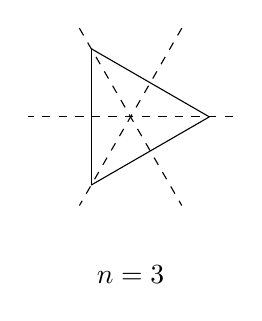
\begin{tikzpicture}[baseline=(0:0cm)]
		\foreach \x in {0,120,240}
			\draw (\x :1cm) -- (\x + 120 :1cm);
		\foreach \x in {0,60,120}
			\draw[dashed] (\x :1.3cm) -- (\x + 180 :1.3cm);
		\node at (270:2cm) {$n=3$};
	\end{tikzpicture} \qquad 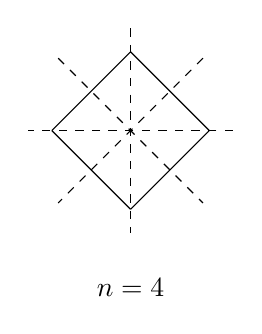
\begin{tikzpicture}[baseline=(0:0cm)]
		\foreach \x in {0,90,...,270}
			\draw (\x :1cm) -- (\x + 90 :1cm);
		\foreach \x in {0,45,...,135}
			\draw[dashed] (\x :1.3cm) -- (\x + 180 :1.3cm);
		\node at (270:2cm) {$n=4$};
	\end{tikzpicture} \qquad 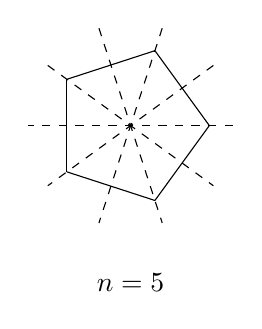
\begin{tikzpicture}[baseline=(0:0cm)]
		\foreach \x in {0,72,...,288}
			\draw (\x :1cm) -- (\x + 72 :1cm);
		\foreach \x in {0,36,...,144}
			\draw[dashed] (\x :1.3cm) -- (\x + 180 :1.3cm);
		\node at (270:2cm) {$n=5$};
	\end{tikzpicture}\end{center}
	子群 $N = \Z/n\Z$ 对应到保持正 $n$ 边形的旋转 ($k + n\Z$ 的转角为 $\frac{2\pi k}{n}$), 剩下 $n$ 个元素是对图中各虚线的镜射, 例如 $\tau$ 可取为对水平轴的镜射. 请读者试着验证.
\end{example}

表法 $G = NH \simeq N \rtimes H$ 也称为内半直积分解, 因为 $NH$ 由群 $G$ 自身的乘法结构描述, 而 $N \rtimes H$ 可谓是从外部构造的. 它们是一体两面, 不必强作区分. 对于直积, 我们还可以刻画多变元的情形.
\begin{lemma}\label{prop:internal-direct}
	设 $G_1, \ldots, G_n$ 为群 $G$ 的子群, 假设
	\begin{compactitem}
		\item 对每个 $i$ 皆有 $G_i \lhd G$,
		\item 对每个 $i$ 皆有 $G_i \cap (G_1 \cdots \widehat{G_i} \cdots G_n) = \{1\}$, 其中 $\widehat{\cdots}$ 表示略去该项,
	\end{compactitem}
	则 $G_i$, $G_j$ 的元素对乘法相交换 ($i \neq j$), 此时 $G_1 \cdots G_n$ 是 $G$ 的正规子群, 而且
	\begin{align*}
		\prod_{i=1}^n G_i & \stackrel{\sim}{\longrightarrow} G_1 \cdots G_n \\
		(g_1, \ldots, g_n) & \longmapsto g_1 \cdots g_n.
	\end{align*}
	 当 $G = G_1 \cdots G_n$ 时, 此同构 $\prod_i G_i \rightiso G$ 称作 $G$ 的\emph{内直积}分解.
\end{lemma}
\begin{proof}
	乘法交换性和 $n=2$ 的情形已经包含于引理 \ref{prop:internal-semidirect}; 由此亦可推出对任意子列 $1 \leq i_1 < \cdots < i_m \leq n$, 乘积 $G_{i_1} \cdots G_{i_m}$ 仍为 $G$ 的正规子群. 对 $n$ 用引理 \ref{prop:internal-semidirect} 递归地论证就得到一般情形.
\end{proof}

\begin{definition}[正合列] \label{def:exact-seq-group}\index{zhenghelie@正合列 (exact sequence)}
	考虑一列群同态
	\[ \cdots \xrightarrow{f_0} G_1 \xrightarrow{f_1} G_2 \xrightarrow{f_2} \cdots \xrightarrow{f_i} G_{i+1} \to \cdots, \]
	长度或有限或无限. 若对所有 $i$ 都有
	\[ \Image(f_i) = \Ker(f_{i+1}), \]
	则称此列\emph{正合}. 我们经常把 $\{1\}$ 简写为 $1$, 或用加性符号记为 $0$. 举例明之, 对于任意同态 $\varphi: G \to G'$, 列 $G \to G' \to 1$ 正合当且仅当 $\varphi$ 是满的, 列 $1 \to G \to G'$ 正合当且仅当 $\varphi$ 是单的, 而我们恒有正合列
	\[ 1 \to \Ker(\varphi) \to G \xrightarrow{\varphi} \Image(\varphi)  \to 1 \]
	其中 $\Ker(\varphi) \to G$ 是自然的包含映射.
\end{definition}
正合列经常和交换图表 (见 \S\ref{sec:cat-and-morphism}) 搭配. 其妙用在同调代数中才会完全彰显.

形如
\[ 1 \to N \to G \xrightarrow{p} H \to 1 \]
的正合列称为\emph{群扩张}. 若有群同态的交换图表\index{qunkuozhang@群扩张 (group extension)}
\[\begin{tikzcd}
	1 \arrow[r] & N \arrow[r] \arrow[equal, d] & G \arrow[r, "p"] \arrow[d, "\varphi"] & H \arrow[equal, d] \arrow[r] & 1 \\
	1 \arrow[r] & N \arrow[r] & G' \arrow[r, "{p'}"'] & H \arrow[r] & 1
\end{tikzcd}\]
其横行皆是群扩张, 则称 $\varphi$ 是群扩张的等价. 不难验证此时 $\varphi$ 必为同构. 对于给定的 $H$ 和 $N$, 群扩张在等价意义下的分类是代数学中不时碰到的问题.

对于群扩张 $1 \to N \to G \xrightarrow{p} H \to 1$, 同态 $s: H \to G$ 若满足 $p s = \identity_H$, 则称为该扩张的一个\emph{分裂}. 由此可建立半直积与可裂扩张的联系, 细说如下.
\begin{enumerate}
	\item 设 $G = N \rtimes_\alpha H$ 为半直积, 则有可裂的群扩张
		\[ \begin{tikzcd}
			1 \arrow[r] & N \arrow[r] & G \arrow[r, "p"] & H \arrow[bend left=30, l, "s"] \arrow[r] & 1
		\end{tikzcd} \]
		其中 $p: G \to H$ 是投影同态 $(n, h) \mapsto h$, 而 $s: H \hookrightarrow G$ 是包含同态 $s(h) = (1,h)$.
	\item 反之, 给定如上的群扩张及其分裂 $s$, 定义 $\alpha: H \to \Aut(N)$ 为伴随自同构 $\alpha(h) = \Ad(s(h))|_N$, 则有群扩张的等价
		\[ \begin{tikzcd}
			1 \arrow[r] & N \arrow[r] \arrow[equal, d] & N \rtimes_\alpha H \arrow[r] \arrow[d, "\varphi"] & H \arrow[equal, d] \arrow[r] & 1 \\
			1 \arrow[r] & N \arrow[r] & G \arrow[r] & H \arrow[r] & 1
		\end{tikzcd} \]
		其中 $\varphi(n, h) := n s(h)$. 请读者验证 $\varphi$ 确实是一对一的群同态.
\end{enumerate}

\section{群作用和计数原理}\label{sec:group-action}
无论从实际应用还是历史的发展观之, 抽象的群往往都由它在某集合上的作用所描述, 而考察种种群作用又是研究群性质的重要手段. 本节的第一个目的是澄清群作用的基本概念.

\begin{definition}[幺半群作用]\label{def:monoid-action} \index{qunzuoyong@群作用 (group action)}
	设 $X$ 为集合, $M$ 为幺半群. $M$ 在 $X$ 上的作用定义为一个映射
	\[ a: M \times X \to X, \]
	称为作用映射, 它必须满足以下性质
	\begin{compactenum}[(i)]
		\item 对所有 $g,g' \in M$ 和 $x \in X$, 有 $a(g', a(g, x)) = a(g'g, x)$ (结合律),
		\item 对所有 $x \in X$, 有 $a(1, x)=x$.
	\end{compactenum}
	带有 $M$ 作用的集合称为 $M$-集. 对所有 $m,x$ 皆有 $a(m,x)=x$ 的作用称为\emph{平凡作用}. $M$-集间的映射 $f: X \to Y$ 若满足
	\[ f(a(m, x)) = a(m, f(x)), \quad m \in M, x \in X \]
	则称为 $M$-\emph{等变}映射. 若等变映射
	\begin{tikzcd}
		M_1 \arrow[yshift=0.5ex, r, "f"] & M_2 \arrow[yshift=-0.5ex, l, "g"]
	\end{tikzcd}
	满足 $fg = \identity_{M_2}$, $gf = \identity_{M_1}$, 则称 $f, g$ 为互逆的同构. 由此可以定义 $M$-集之间的同构概念.
\end{definition}

\begin{remark}
	一句话, 给定 $M$, 全体 $M$-集连同等变映射构成一范畴 $M\dcate{Set}$. 这里严格地说也得限制 $M$-集 $X$ 的大小, 必须假设 $M$, $X$ 同属选定的宇宙 $\mathcal{U}$, 详见定义 \ref{def:U-cat} 及相关讨论.
\end{remark}

% 倘若用例 \ref{eg:symmetric-group} 的语言, 那么给定 $M$ 在 $X$ 上的作用相当于给定同态 $M \to \Aut(X)$: 它将每个 $m \in M$ 映至双射 $\left[ x \mapsto a(m,x) \right] \in \Aut(X)$.

习惯将 $M$-集带有的作用映射略去, 并将 $a(m, x)$ 写成 $m \cdot x$ 或 $mx$. 作用映射的条件和等变性遂有自然的写法
\begin{gather*}
	m'(mx) = (m'm)x, \\
	1 \cdot x = x, \\
	f(mx) = mf(x),
\end{gather*}
其中 $ m, m' \in M, x \in X$. 这般定义的作用称为 $M$ 的左作用, 因以 $M$ 的左乘表示之故. 我们同样可以定义 $M$ 的右作用 $(x, m) \mapsto xm$. 上述定义可以逐条改写, 例如 $(xm)m' = x(mm')$ 等. 一劳永逸的方法则是利用对偶性: $M$ 的右作用无非是 $M^\text{op}$ 的左作用. 本节针对左作用的陈述都有相应的右版本, 不再赘述.

\begin{example}
	对任意集合 $X$, 对称群 $\mathfrak{S}_X$ 当然地作用于 $X$ 上: $a: (\sigma, x) \mapsto \sigma(x)$. 类似地, 实 $n \times n$ 矩阵所成幺半群 $M_n(\R)$ 作用于 $\R^n$: 视 $\R^n$ 元素为 $n \times 1$ 阶竖直矩阵, 则作用 $(A, x) \mapsto A x$ 无非是矩阵乘法.
\end{example}

\begin{example}
	若群 $G$ 左作用于 $X$, 而 $Y$ 是任意集合, 则 $G$ 在 $\{f: \text{映射}\; X \to Y \}$ 上有自然的左作用 $a(g,f) = \left[ x \mapsto f(g^{-1}x) \right]$; 若 $G$ 右作用于 $X$, 则相应的左作用取为 $[x \mapsto f(xg)]$. 请读者验证细节.
\end{example}

\begin{example}
	以下讨论可参看 \cite[例 7.2.4]{Zh2}. 设 $n \geq 1$, 空间 $C_\infty(\R^n)$ 为速降函数空间 $\mathscr{S}(\R^n)$ (参看 \cite[例 3.2.7]{Zh1}) 在 $L^\infty(\R^n)$  中的闭包. 定义幺半群 $(\R_{\geq 0}, +)$ 在 $C_\infty(\R^n)$ 上的作用如下:
	\[ a(t, u) =
		\begin{cases}
			G_t \ast u, & t > 0, \\
			u, & t=0,
		\end{cases}\]
	其中 $\ast$ 是卷积而 $G_t$ 是 $\R^n$ 上熟知的热核函数
	\[ G_t(x) := (4\pi t)^{-\frac{n}{2}} e^{-\|x\|^2 /4t}, \quad x \in \R^n. \]
	根据热传导方程的理论, $v(t, \cdot) := a(t, u)$ 满足初值问题 $\frac{\partial v}{\partial t} = \Delta v$, $v(0, \cdot) = u(\cdot)$, 因此 $a$ 的确给出幺半群作用. 泛函分析中称此为算子(幺)半群. 由于热传导磨光函数的奇点, 此作用无法延拓到群 $(\R, +)$.
\end{example}

\begin{definition}\index{guidao@轨道 (orbit)}\index{wendinghuazi@稳定化子 (stabilizer)}\index[sym1]{Stab@$\Stab$}
	设幺半群 $M$ 作用于 $X$. 定义
	\begin{compactitem}
		\item \emph{不动点}集 $X^M := \{x \in X: \forall m \in M, \; mx=x \}$;
		\item 对于 $x \in X$, \emph{轨道} $Mx := \{mx : m \in M \}$, 其元素称为该轨道的代表元, 轨道 $Mx$ 是 $X$ 的 $M$-子集;
		\item 承上, 其\emph{稳定化子}定为 $M$ 的子幺半群 $\Stab_M(x) := \{m \in M : mx=x\}$.
	\end{compactitem}
\end{definition}

最常用的作用还是群作用. 对于群 $G$, 作用的基本构件是形如 $G/H$ 的陪集空间, 其作用映射由 $(g, xH) \mapsto gxH$ 给出. 以下结果告诉我们如何将一般的 $G$-集分解成陪集空间的无交并. 这也是计数原理的出发点.

\begin{lemma}\label{prop:orbit-decomp}
	设群 $G$ 作用于 $X$, 则
	\begin{compactenum}[(i)]
		\item 有轨道分解 $X = \bigsqcup_x Gx$, 其中我们对每个轨道选定代表元 $x$;
		\item 对每个 $x \in X$, 映射
			\begin{align*}
				G/\Stab_G(x) & \longrightarrow Gx \\
				g \cdot \Stab_G(x) & \longmapsto gx
			\end{align*}
			是 $G$-集间的同构;
		\item 特别地, 我们有基数的等式 (参看 \eqref{eqn:cardinal-infinite-sum})
			\[ |X| = \sum_x \left( G: \Stab_G(x) \right); \]
		\item 对所有 $x \in X$ 和 $g \in G$, 有
			\[ \Stab_G(gx) = g \Stab_G(x) g^{-1}. \]
	\end{compactenum}
\end{lemma}
\begin{proof}
	首先证明若两轨道 $Gx, Gy$ 有交, 则 $Gx=Gy$. 诚然, 若 $gx=g'y$, 则 $x = g^{-1}g' y \in Gy$, 故 $Gx \subset Gy$; 由对称性导出 $Gx=Gy$. 由 $\forall x, \; x = 1\cdot x \in Gx$ 立得轨道分解. 关于映射 $G/\Stab_G(x) \to Gx$ 的断言是稳定化子定义的直接推论. 配合轨道分解便导出基数等式. 最后一个等式可径由定义验证.
\end{proof}

由此可见性质 ``$x,y$ 属同一轨道''给出 $X$ 上的等价关系. 相应的商集或曰轨道空间记为 $G \backslash X$; 对于右作用, 轨道空间自然就记为 $X/G$. 留意到给定 $G$ 在 $X$ 上的作用相当于给定同态 $G \to \mathfrak{S}_X$, 它映 $g$ 为 $[x \mapsto gx]$.
\begin{definition}
	设 $G$ 为群, $X$ 为 $G$-集, 我们称 $G$ 在 $X$ 上的作用是 \index{qunzuoyong!忠实 (faithful)}\index{qunzuoyong!传递 (transitive)}
	\begin{compactitem}
		\item 忠实的, 如果相应的 $G \to \mathfrak{S}_X$ 是单射, 这相当于 $\bigcap_{x \in X} \Stab_G(x) = \{1\}$;
		\item 自由的或单的, 如果对任意 $x \in X$ 都有 $\Stab_G(x) = \{1\}$;
		\item 传递的, 如果 $X$ 仅有一个轨道, 这相当于要求 $X$ 非空, 并且对所有 $x, y \in X$ 皆存在 $g \in G$ 使得 $gx=y$;
		\item 推而广之, 若对每个 $1 \leq m \leq n$, 群 $G$ 在 $\{ (x_1, \ldots, x_m) \in X^m: \text{相异元} \}$ 上的作用皆传递, 则称 $G$ 在 $X$ 上的作用为 $n$-传递的.
	\end{compactitem}

	传递的 $G$-集又称 $G$-\emph{齐性空间}, 自由的 $G$-齐性空间称为 $G$-\emph{主齐性空间}或\emph{挠子}.\index{qixingkongjian@齐性空间 (homogeneous space)}\index{naozi@挠子 (torsor)}
\end{definition}
作为引理 \ref{prop:orbit-decomp} 的推论, 陪集空间 $G/H$ 在同构意义下穷尽了所有齐性空间.

这些术语有显然的几何渊源, 为此必须引入流形结构及底空间. 然而本节考虑的仅有集合, 主要的应用在于集合的计数问题, 详见 \S\ref{sec:Sylow}.  我们且先看些一般例子.

\begin{example}[平移作用与陪集]
	设 $G$ 为群而 $H$ 为其子群, 则 $H$ 在 $G$ 上的左作用 $(h, g) \mapsto hg$ 称为左平移作用. 易见
	\begin{inparaenum}[(i)]
		\item 相应的轨道无非是陪集 $Hg$ ($g \in G$),
		\item 轨道空间无非是陪集空间 $H \backslash G$,
		\item 此作用是自由的, 它是传递的当且仅当 $H=G$.
	\end{inparaenum}
	这些断言对 $H$ 在 $G$ 上的右平移作用 $(g,h) \mapsto gh$ 同样成立, 相应的轨道空间无非是 $G/H$.

	现在设 $H, K$ 为 $G$ 的子群. 双陪集有类似的解读: 考虑 $H \times K^\text{op}$ 在 $G$ 上的左作用
	\[ ((h, k), g) \mapsto hgk, \quad (h, k) \in H \times K^\text{op}, \; g \in G. \]
	相应的轨道正好是双陪集 $HgK$ ($g \in G$), 轨道空间等同于 $H \backslash G/K$. 但此作用的其它性质则远比左陪集或右陪集的情形复杂.
\end{example}

\begin{example}[共轭作用]\label{eg:conj-action} \index{gonge@共轭 (conjugation)}
	依旧设 $G$ 为群. 伴随自同构 $\Ad: G \to \Aut(G)$ 给出的作用称为 $G$ 的\emph{共轭作用} $G \times G \to G$ (在此考虑左作用). 定义展开后无非是
	\[ (g, x) \longmapsto {}^g x := gxg^{-1}. \]
	共轭作用下的轨道称为 $G$ 中的\emph{共轭类}.

	推而广之, 对任意子集 $E \subset G$ 我们业已定义子群 $N_G(E)$, 它在 $E$ 上的作用也叫共轭. 若两子集 $E, E'$ 满足 $\exists g \in G, \; E' = gEg^{-1}$, 则称 $E$ 与 $E'$ 共轭.

	非交换群共轭作用的性状一般相当复杂. 对于 $x \in G$, 其稳定化子群正是中心化子 $Z_G(x)$, 而不动点集则是中心 $Z_G$. 剖析 $G$ 的共轭作用是了解其群结构的必由之路.
\end{example}

挠子是一类特别常见的 $G$-集, 这套语言需要有合适的几何背景方能发力: 参看 \S\ref{sec:group-in-cat}. 以下仅介绍最初步的例子.
\begin{example}
	设 $G_1$, $G_2$ 为群, 置
	\[ \Isom(G_1, G_2) := \{ \text{ 同构 } \; \varphi: G_1 \to G_2 \}. \]
	当 $\Isom(G_1, G_2)$ 非空时, 其上有 $\Aut(G_2)$ 的左作用 $(g, \varphi) \mapsto g \circ \varphi$, 其中 $g \in \Aut(G_2)$. 这使得 $\Isom(G_1, G_2)$ 成为 $\Aut(G_2)$-挠子. 虽然这里只考虑群同构, 类似构造实则可以在任意范畴中进行, 请参见 \S\ref{sec:cat-and-morphism}.

	我们当然不必自限于左作用, $\Aut(G_1)$ 也借映射合成右作用于 $\Isom(G_1, G_2)$, 两侧的作用满足 $(g \circ \varphi) \circ g' = g \circ (\varphi \circ g')$, 故可并作 $\Aut(G_1)^{\text{op}} \times \Aut(G_2)$-作用, 无论左看右看 $\Isom(G_1, G_2)$ 都是挠子. 这样的结构称为双挠子.
\end{example}

挠子原来的定义稍显曲折, 然而它另有简捷的刻画如下, 在范畴论的框架中将会格外方便; 可参看 \S\ref{sec:group-in-cat}.

\begin{lemma}\label{prop:torsor-criterion}
	设 $X$ 为非空 $G$-集, 则 $X$ 为挠子当且仅当映射
	\begin{align*}
		\Phi: G \times X & \longrightarrow X \times X \\
		(g, x) &  \longmapsto (x, gx)
	\end{align*}
	是双射.
\end{lemma}
\begin{proof}
	据定义 $\Phi^{-1}(x,y) = \{g \in G: gx=y\}$. 因此映射 $\Phi$ 是单射当且仅当 $X$ 自由, 是满射当且仅当 $X$ 传递.
\end{proof}

\section{Sylow 定理}\label{sec:Sylow}
首先引入 $p$-群的概念.

\begin{definition}\label{def:p-group}\index{$p$-群}
	设 $p$ 为素数. 满足 $|G|=p^m$, $m \in \Z_{\geq 0}$ 的群 $G$ 称为 $p$-群.
\end{definition}
应用命题 \ref{prop:Lagrange}, 易见 $p$-群的子群和商群仍是 $p$-群.

\begin{proposition}\label{prop:counting-localization}
	设 $G$ 为非平凡 $p$-群, 则任意有限 $G$-集 $X$ 皆满足
	\[ |X| \equiv \left\lvert X^G \right\rvert \mod p. \]
\end{proposition}
\begin{proof}
	对任意 $x \in X$, 命题 \ref{prop:Lagrange} 蕴涵 $(G: \Stab_G(x))$ 是 $p$ 的幂. 故有
	\[ [ x \notin X^G] \iff [ \Stab_G(x) \neq G ] \iff (G: \Stab_G(x)) \equiv 0 \bmod p . \]
	套入引理 \ref{prop:orbit-decomp} 即得所求.
\end{proof}

\begin{corollary}\label{prop:p-group-center}
	设 $G$ 为非平凡的 $p$-群, 则 $Z_G \neq \{1\}$.
\end{corollary}
\begin{proof}
	考虑 $G$ 的共轭作用 (例 \ref{eg:conj-action}). 由命题 \ref{prop:counting-localization} 得到
	\[ 0 \equiv |G| \equiv |Z_G| \mod p , \]
	故 $|Z_G| > 1$.
\end{proof}

此式可用以递归地研究 $p$-群的结构, 兹举一例.
\begin{corollary}
	设 $G$ 为 $p$-群而 $H \subsetneq G$ 为真子群, 则 $H \subsetneq N_G(H)$. 特别地, $(G:H)=p$ 蕴涵 $H \lhd G$.
\end{corollary}
\begin{proof}
	已知 $Z_G$ 非平凡, 显然 $Z_G \subset N_G(H)$. 若 $Z_G \not\subset H$, 则 $H \subsetneq Z_G H \subset N_G(H)$. 因此不妨假设 $Z_G \subset H$. 现在对 $|G|$ 递归论证: 定义 $\bar{G} := G/Z_G$, $\bar{H} := H/Z_G$, 可假设
	\[ \bar{H} \subsetneq N_{\bar{G}}(\bar{H}). \]
	容易看出 $N_G(H)/Z_G = N_{\bar{G}}(\bar{H})$. 应用命题 \ref{prop:2nd-homomorphism} 即得 $H \subsetneq N_G(H)$.
\end{proof}

另一个直接而重要的推论如下. 先回忆我们在 \S\ref{sec:group-and-monoid} 定义的元素 $x \in G$ 的阶 $\text{ord}(x)$.
\begin{corollary}[Cauchy 定理]\label{prop:group-Cauchy}
	设 $G$ 为有限群, 素数 $p$ 整除 $|G|$, 则存在 $x \in G$ 使得 $\ord(x)=p$.
\end{corollary}
\begin{proof}
	定义集合
	\[ X_p := \{(g_i)_{1 \leq i \leq p} \in G^p : g_1 \cdots g_p = 1 \}. \]
	不妨将下标 $1 \leq i \leq p$ 看成 $\Z/p\Z$ 里的元素. 如此一来循环群 $\Z/p\Z$ 就作用在 $X_p$ 上: 陪集 $m + p\Z$ 的作用是平移下标
	\[ (g_i)_{i \in \Z/p\Z} \longmapsto (g_{i+m})_{i \in \Z/p\Z}. \]
	须证明此作用不逸出 $X_p$, 仅须检查 $m=1$ 的情形: 对等式 $g_1 \cdots g_p = 1$ 左乘以 $g_1^{-1}$, 右乘以 $g_1$ 即是. 由此导出 $(X_p)^{\Z/p\Z} = \{(x, \ldots, x) : x^p = 1 \}$. 注意到 $x^p=1$ 且 $x \neq 1$ 等价于 $\ord(x)=p$ (参看例 \ref{eg:cyclic-group}).

	由于 $g_p = (g_1 \cdots g_{p-1})^{-1}$, 投影映射 $X_p \to G^{p-1}$, $(g_i)_{1 \leq i \leq p} \mapsto (g_i)_{1 \leq i < p}$ 是双射, 故
	\[ |X_p| = |G|^{p-1} \equiv 0 \mod p. \]
	另一方面, 命题 \ref{prop:counting-localization} 给出
	\[ |X_p| \equiv \left\lvert(X_p)^{\Z/p\Z}\right\rvert = 1 + \left\lvert \{x \in G : \ord(x)=p \} \right\rvert \mod p , \]
	故 $\{x \in G : \ord(x)=p \}$ 非空.
\end{proof}

\begin{convention}
	设 $p$ 为素数, $n \in \Z_{\geq 1}$, 若 $p^a \mid n$ 而且 $p^{a+1} \nmid n$, 则写作 $p^a \| n$.
\end{convention}

\begin{definition}\index{Sylow $p$-子群}
	设 $G$ 为 $n$ 阶有限群, $p$ 为素数. 设 $p^m \| n$, 满足 $|H| = p^m$ 的子群 $H$ 称为 $G$ 的 Sylow $p$-子群.
\end{definition}
这意谓 $p$-子群 $H$ 在 Lagrange 定理的约束下达到最大可能阶数. 此定义显然仅在 $p \mid n$ 时才有实质意涵.

\begin{lemma}\label{prop:Wielandt-lemma}
	设 $p$ 为素数. 对任意非负整数 $b \leq a$, $a \neq 0$ 和 $m$, 二项式系数满足同余式
	\[ \binom{p^m a}{p^m b} \equiv \binom{a}{b} \mod p. \]
\end{lemma}
\begin{proof}
	考虑以符号 $T$ 为变元的整系数多项式. 由于 $0 < c < p \implies p \mid \binom{p}{c}$, 故
	\[ (T+1)^{pa} = \left( T^p + p(\cdots) + 1 \right)^a \equiv (T^p + 1)^a \mod p. \]
	即: 两边逐系数模 $p$ 同余. 两侧以二项式定理展开, 比较 $T^{pb}$ 的系数即得 $m=1$ 的情形. 迭代 $m$ 次遂得一般情形.
\end{proof}

\begin{theorem}[Sylow 第一定理]
	对任意素数 $p$, 任意有限群 $G$ 含有 Sylow $p$-子群.
\end{theorem}
下面论证供鉴赏之用, 另有它证如 \cite[Theorem 6.2]{Lang02}.
\begin{proof}[H.\ Wielandt]
	置 $n := |G|$, 不妨假设 $p^m \| n$, $m \geq 1$. 定义
	\[ Y := \left\{ \text{ 子集 } \; E \subset G : |E|=p^m \right\}. \]
	由引理 \ref{prop:Wielandt-lemma} 知
	\[ |Y| = \binom{n}{p^m} \equiv \binom{p^{-m} n}{1} = p^{-m} n \not\equiv 0 \mod p . \]

	群 $G$ 以左平移 $(g, E) \mapsto gE$ 作用于 $Y$. 由引理 \ref{prop:orbit-decomp} 和以上同余式知存在 $E \in Y$ 使得 $p \nmid (G: \Stab_G(E))$, 我们断言 $H := \Stab_G(E)$ 是 Sylow $p$-子群. 首先注意到 $p \nmid \frac{|G|}{|H|}$ 故 $p^m$ 整除 $|H|$. 任取 $g \in E$, 由稳定化子的性质知 $Hg  \subset E$; 配合 $|H|=|Hg|$ 遂得到 $|H| \leq  |E| = p^m$, 故 $|H|=p^m$. 明所欲证.
\end{proof}

\begin{lemma}
	设 $p$ 为素数, 而$P$ 是 $G$ 的 Sylow $p$-子群. 若 $G$ 的 $p$-子群 $H$ 满足 $H \subset N_G(P)$, 则 $H \subset P$.
\end{lemma}
\begin{proof}
	对群 $HP$ 应用命题 \ref{prop:3rd-homomorphism} 可得群同构 $HP/P \simeq H/H \cap P$, 故 $HP$ 仍是 $p$-群. 又因为 $P \subset HP \subset G$ 而 $P$ 是 Sylow $p$-子群, 必有 $HP=P$, 而这又等价于 $H \subset P$.
\end{proof}

\begin{theorem}[Sylow 第二定理]
	令 $G$ 为有限群, $p$ 为素数. 则
	\begin{compactenum}[(i)]
		\item 任意 $p$-子群 $H \subset G$ 皆包含于某个 Sylow $p$-子群;
		\item $G$ 的任两个 Sylow $p$-子群 $P, P'$ 皆共轭;
	\end{compactenum}
	特别地, $G$ 中存在正规的 Sylow $p$-子群 当且仅当 $G$ 有唯一的 Sylow $p$-子群.
\end{theorem}
\begin{proof}
	选定 Sylow $p$-子群 $P \subset G$, 并考虑它在 $G$ 的共轭作用下的轨道
	\[ X := \left\{ gPg^{-1} : g \in G \right\} \]
	任意 $Q \in X$ 都是 $G$ 的 Sylow $p$-子群, 而且其稳定化子群是 $N_G(Q)$. 我们有 $G$-集的同构
	\begin{align*}
		G/N_G(P) & \stackrel{\sim}{\longrightarrow} X \\
		g N_G(P) & \longmapsto gPg^{-1}.
	\end{align*}

	由于 $P \subset N_G(P)$, 我们有 $|X| \not\equiv 0 \mod p$. 现假设 $H \subset G$ 为 $p$-子群, 那么 $H$ 也共轭作用于 $X$ 上. 应用命题 \ref{prop:counting-localization} 得 $X^H$ 非空. 取 $Q \in X^H$, 从定义知 $H \subset N_G(Q)$, 上述引理遂保证 $H \subset Q$, 这就证明了第一个断言. 若进一步要求 $H$ 为  Sylow $p$-子群, 则必有 $H = Q$. 由于 $X$ 中元素相互共轭, 第二个断言随之得证.
\end{proof}

\begin{theorem}[Sylow 第三定理]
	承上, $G$ 中 Sylow $p$-子群的个数 $\equiv 1 \mod p$.
\end{theorem}
\begin{proof}
	沿用上个证明的框架, 选定 Sylow $p$-子群 $P$ 并取 $H = P$, 以上业已证明了 $X^P$ 中的元素必为包含 $P$ 的 $p$-子群, 故 $X^P = \{P\}$. 套回命题 \ref{prop:counting-localization} 遂得 $|X| \equiv \left\lvert X^P \right\rvert = 1 \mod p$.
\end{proof}

\begin{proposition}
	 对每个素数 $p$, 有限群 $G$ 的每个 Sylow $p$-子群皆正规的充分必要条件是 $G = \prod_{p \mid\; |G|} H_p$, 其中 $H_p$ 是 $p$-子群.
\end{proposition}
\begin{proof}
	设 $p_1 < \cdots < p_r$ 为素数. 若 $G$ 同构于直积 $\prod_{i=1}^r H_{p_i}$, 其中 $|H_{p_i}| = p_i^{a_i}$ ($a_i \in \Z_{\geq 1}$), 那么 $H_{p_i}$ 自然地嵌入为 $G$ 的正规 Sylow $p_i$-子群, 而 $|G| = \prod_{i=1}^r p_i^{a_i}$.
	
	反过来设 $|G| = p_1^{a_1} \cdots p_r^{a_r}$, 而且对每个 $1 \leq i \leq r$ 皆有正规 Sylow $p_i$-子群 $H_{p_i}$. 它们的阶数两两互素, 运用命题 \ref{prop:Lagrange} 可以在 $G$ 中验证 $H_{p_i} \cap \prod_{j \neq i} H_{p_j} = \{1\}$. 于是引理 \ref{prop:internal-direct} 的条件成立, 得到同构 $\prod_{i=1}^r H_{p_i} \rightiso H_{p_1} \cdots H_{p_r} \subset G$. 比较阶数可知 $H_{p_1} \cdots H_{p_r} = G$.
\end{proof}

\section{群的合成列}\label{sec:composition-series-grp}
将一个群设法拆解为较小的构件是群论的常见手法, 合成列是其中一例.

\begin{definition}[正规列]\label{def:normal-series}\index{zhengguilie@正规列 (normal series)}
	群 $G$ 的递降子群链
	\[ G = G_0 \supset G_1 \supset \cdots \supset G_n = \{1\} \]
	如满足 $\forall 0 \leq i < n,\;  G_{i+1} \lhd G_i$, 则称之为\emph{正规列}, 而群族
	\[ G_i/G_{i+1}, \quad i=0, \ldots, n-1 \]
	称为该列的\emph{子商}. 正规列的\emph{加细}是透过形如 \index{zishang@子商 (subquotient)}
	\[ \left[ \cdots \supset G_i \supset G_{i+1} \supset \cdots \right] \leadsto \left[ \cdots \supset G_i \supset G' \supset G_{i+1} \supset \cdots \right] \]
	的反复插项得到的新列. 插入 $G' = G_i$ 或 $G_{i+1}$ 得到的加细是平凡的; 反之则称为\emph{真加细}.
\end{definition}

下节将考虑一种特殊的正规列, 在此一并定义.
\begin{definition}[中心列]\label{def:central-series}\index{zhongxinlie@中心列 (central series)}
	群 $G$ 的正规列 $G = G_0 \supset G_1 \supset \cdots$ 如对每个 $i$ 都满足
	\begin{gather*}
		G_i \lhd G, \\
		G_i/G_{i+1} \subset Z_{G/G_{i+1}},
	\end{gather*}
	则称为\emph{中心列}.
\end{definition}

\begin{definition}[合成列]\label{def:composition-series}\index{hechenglie@合成列 (composition series)}
	若群 $G$ 的正规列 $G = G_0 \supset G_1 \supset \cdots$ 满足 $G_{i+1} \subsetneq G_i$, 而且子商皆为单群, 则称之为\emph{合成列}.
\end{definition}
细观单群定义可见合成列正是无冗余项, 而且无法再(真)加细的列. 有限群总有合成列, 一般的群则未必.

\begin{lemma}[Zassenhaus 引理]\label{prop:Zassenhaus}
	固定群 $G$, 考虑子群 $U, V$ 及各自的正规子群 $u \lhd U$, $v \lhd V$. 则有
	\begin{gather*}
		u(U \cap v) \lhd u(U \cap V), \\
		(u \cap V) v \lhd (U \cap V)v,
	\end{gather*}
	其中各项在注记 \ref{rem:HN} 的意义下都是子群, 而且有自然的同构
	\[ \dfrac{u (U \cap V)}{u (U \cap v)} \simeq \dfrac{(U \cap V)v}{(u \cap V)v}. \]
\end{lemma}
\begin{proof}
	我们将表解各子群之间的关系, 图例如下:
	\[ \begin{tikzcd}
		G \arrow[dash, d] \\ H: \text{子群}
	\end{tikzcd} \quad
	\begin{tikzcd}
		G \arrow[dash, d, "\triangledown" description] \\ N: \text{正规子群}
	\end{tikzcd} \quad
	\begin{tikzcd}[column sep=tiny]
		A \arrow[dash, rd] & & B \arrow[dash, ld] \\
		& A \cap B &
	\end{tikzcd} \quad
	\begin{tikzcd}[column sep=tiny]
		{}& HN \arrow[dash, ld] \arrow[dash, rd, "\triangledown" description] & \\
		H & & N
	\end{tikzcd}\]
	其中 $H \subset N_G(N)$. 现断言有以下图表:
	\[ \begin{tikzcd}[column sep=tiny]
		{} & U \arrow[dash, d] & & V \arrow[dash, d] & \\
		& u(U \cap V) \arrow[dash, dd, "\triangledown" description] \arrow[dash, rd] & & (U \cap V)v \arrow[dash, dd, "\triangledown" description] \arrow[dash, ld] & \\
		& & U \cap V \arrow[dash, dd, "\triangledown" description] & & \\
		& u(U \cap v) \arrow[dash, ld] \arrow[dash, rd] & & (u \cap V)v \arrow[dash, ld] \arrow[dash, rd] & \\
		u \arrow[dash, rd] & & (u \cap V)(U \cap v) \arrow[dash, ld] \arrow[dash, rd] & & v \arrow[dash, ld] \\
		& u \cap V & & U \cap v &
	\end{tikzcd} \]
	首先留意有性质 $U \cap V \subset N_G(u) \cap N_G(v)$ 等等, 图中的积 $u(U \cap V)$ 等因而是子群. 图例第一条 (即: 子群在下) 显然成立. 又可逐一验证
	\begin{align*}
		u(U \cap v) \cap (U \cap V) & = (u \cap V)(U \cap v) = (U \cap V) \cap (u \cap V)v, \\
		u \cap (u \cap V)(U \cap v) & = u \cap V, \\
		(u \cap V)(U \cap v) \cap v & = U \cap v.
	\end{align*}
	故图例第三条 (子群交) 也成立. 同理可验证图例第四条 (子群积). 至于第二条 (正规子群), 从 $v \lhd V$ 可导出 $U \cap v \lhd U \cap V$, 从而 $u(U \cap v) \lhd u(U \cap V)$; 同理有 $(u \cap V)v \lhd (U \cap V)v$, 取交即得 $(u \cap V)(U \cap v) \lhd U \cap V$. 至此证成断言.

	现在考虑图表中的两个平行四边形. 分别运用命题 \ref{prop:3rd-homomorphism} 可得自然同构
	\begin{equation*}\begin{tikzcd}[column sep=tiny, row sep=small]
		\dfrac{u (U \cap V)}{u(U \cap v)} \arrow[rd, "\simeq"'] &  & \dfrac{(U \cap V)v}{(u \cap V)v} \arrow[ld, "\simeq"] \\
		& \dfrac{U \cap V}{(u \cap V)(U \cap v)} &
	\end{tikzcd}\end{equation*}
	明所欲证.
\end{proof}

\begin{definition}\label{def:JH-subquotients}
	设 $G = G_0 \supset \cdots$ 为正规列, 我们视其子商 $(G_i/G_{i+1})_{i \geq 0}$ 为不计顺序, 但计入重数的集合. 如果两个正规列长度相同, 而且其子商在上述意义下相等, 则称两正规列\emph{等价}.
\end{definition}

\begin{theorem}[Schreier 加细定理]\label{prop:Schreier}
	设
	\begin{align*}
		G & = G_0 \supset \cdots \supset G_r \supset G_{r+1} = \{1\}, \\
		G & = H_0 \supset \cdots \supset H_s \supset H_{s+1} = \{1\}
	\end{align*}
	为 $G$ 的两个正规列, 则两者有等价的加细.
\end{theorem}
\begin{proof}
	对每个 $0 \leq i \leq r$, $0 \leq j \leq s$ 定义
	\begin{align*}
		G_{i,j} & := G_{i+1} (H_j \cap G_i), \\
		H_{j,i} & := (G_i \cap H_j) H_{j+1}.
	\end{align*}
	先看 $G_{i,j}$, 由 $G_{i+1} \lhd G_i$ 知其为子群. 包含关系 $G_{i, j+1} \lhd G_{i,j}$ 成立, 而且
	\[ G_{i,0} = G_{i+1} (G \cap G_i) = G_i, \quad G_{i,s+1} = G_{i+1}, \]
	遂得到 $(G_i)_{i=0}^r$ 的加细
	\[ \mathcal{G} := \left[ \cdots \supset G_i = G_{i, 0} \supset G_{i, 1} \supset \cdots G_{i, s} \supset G_{i, s+1}= G_{i+1} \supset \cdots \right] . \]
	同理可见 $H_{j, i}$ 给出 $(H_j)_{j=0}^s$ 的加细, 记为 $\mathcal{H}$. 在引理 \ref{prop:Zassenhaus} 中取 $u := G_{i+1}$, $U := G_i$ 和 $v := H_{j+1}$, $V := H_j$, 遂导出
	\[ \dfrac{G_{i,j}}{G_{i,j+1}} = \dfrac{u(U \cap V)}{u(U \cap v)} \simeq \dfrac{(U \cap V)v}{(u \cap V)v} = \dfrac{H_{j,i}}{H_{j,i+1}}. \]

	当 $(i,j)$ 取遍所有可能, 正规列 $\mathcal{G}$, $\mathcal{H}$ 的各个子商在同构两边都恰好出现一次. 证毕.
\end{proof}

\begin{theorem}[Jordan--Hölder 定理]\label{prop:JH-group}\index{Jordan--Hölder 定理}
	群 $G$ 的任两个合成列皆等价.
\end{theorem}
\begin{proof}
	这是定理 \ref{prop:Schreier} 配合定义 \ref{def:composition-series} 的直接推论.
\end{proof}

因此, 一旦群 $G$ 有合成列, 则其子商在定义 \ref{def:JH-subquotients} 的意义下无关合成列的选取.
\begin{definition}\index{hechengyinzi@合成因子 (composition factor)}
	假设群 $G$ 有合成列, 定义其\emph{合成因子}或 Jordan--Hölder 因子集 $\text{JH}(G)$ 为其任意合成列的全体子商 (不计顺序, 计入重数).
\end{definition}

带重数集 $\text{JH}(G)$ 是一种管用的不变量, 但它无法在同构意义下刻画群. 例如群 $\Z/4\Z$ 与 $\Z/2\Z \times \Z/2\Z$ 的合成因子都是 $\{ \Z/2\Z, \Z/2\Z\}$, 但两群不同构.

此外, 给定群的正合列 $1 \to N \to G \xrightarrow{\pi} Q \to 1$. 假设 $N$, $Q$ 皆有合成列, 则 $G$ 亦有合成列, 而且
\begin{gather}\label{eqn:JH-ses}
	\text{JH}(G) = \text{JH}(N) \cup  \text{JH}(Q),
\end{gather}
这里的并集当然是计入重数的. 论证如下: 分别考虑 $Q$ 和 $N$ 的合成列 $(Q_i)_i$, $(N_j)_j$, 两者可以衔接成合成列
\[ G \supset \pi^{-1}(Q_1) \supset \cdots \supset \pi^{-1}(Q_r) = N \supset N_1 \supset \cdots . \]
其合成因子正是 $\text{JH}(N) \cup  \text{JH}(Q)$.

\begin{proposition}\label{prop:abelian-composition-series}
	若 $G$ 为有限交换群, 则 $\text{JH}(G)$ 中的元素都是素数阶群.
\end{proposition}
留意: 素数阶群都是循环群.
\begin{proof}
	可假设 $G$ 非平凡群. 推论 \ref{prop:group-Cauchy} 确保存在素数 $p$ 及 $p$ 阶元素 $t \in G$. 考虑交换群的正合列
	\[ 1 \to \lrangle{t} \to G \to G/\lrangle{t} \to 1 \]
	并利用 \eqref{eqn:JH-ses} 施递归于 $|G|$, 即得所求.
\end{proof}

我们将在推论 \ref{prop:finite-abelian-structure} 详细描述有限交换群的结构.

\section{可解群与幂零群}\label{sec:solvable-groups}
可解群的概念源于 Galois 对高次方程根式解的研究, 幂零与超可解群则是其变体. 这些概念在 Lie 群, Lie 代数的研究中占有重要地位, 本节主要介绍其群论的面向. 请先回忆定义 \ref{def:normal-series}, \ref{def:central-series} 中的子群列.

\begin{definition}\label{def:solvable-nilpotent-group}\index{kejiequn@可解群 (solvable group)}\index{chaokejiequn@超可解群 (supersolvable group)}\index{milingqun@幂零群 (nilpotent group)}
	设 $G$ 为群.
	\begin{enumerate}
		\item 若存在正规列 $G = G_0 \supset G_1 \supset \cdots \supset G_r = \{1\}$ 使得每个子商都交换, 则称之为\emph{可解群};
		\item 承上, 若对每个 $i$ 皆有 $G_i \lhd G$, 且 $G_i/G_{i+1}$ 是素数阶循环群, 则称之为\emph{超可解群};
		\item 如果存在中心列 $G = G_0 \supset G_1 \supset \cdots \supset G_r = \{1\}$, 则称之为\emph{幂零群}.
	\end{enumerate}
\end{definition}

我们希望在上述定义中找到一类典则的正规列/中心列, 借以检验一个群是否可解或幂零. 以下概念是必要的.
\begin{definition}\index[sym1]{$[x,y]$}
	对于 $x, y \in G$, 定义\emph{换位子}
	\[ [x,y] := xyx^{-1}y^{-1}. \]
	对任意子集 $A, B \subset G$, 置 $[A, B] \lhd G$ 为包含 $\{[a,b] : a \in A, b \in B\}$ 的最小正规子群, 或简称为它们生成的正规子群. 递归地定义 $G$ 之
	\begin{itemize}
		\item \emph{导出列}: \begin{tikzpicture}[baseline] \matrix (M) [matrix of math nodes, left delimiter={\{} ] {
			\mathscr{D}^{i+1} G := [\mathscr{D}^i G, \mathscr{D}^i G] \\
			\mathscr{D}^0 G := G, \\
		}; \node at (M-1-1.east) [right=1em] {($i \geq 0$)}; \end{tikzpicture}
		\item \emph{降中心列}: \begin{tikzpicture}[baseline] \matrix (M) [matrix of math nodes, left delimiter={\{} ] {
			\mathscr{C}^{i+1} G := [\mathscr{C}^i G, G] \\
			\mathscr{C}^0 G := G. \\
		}; \node at (M-1-1.east) [right=1em] {($i \geq 0$)}; \end{tikzpicture}
	\end{itemize}
\end{definition}

容易验证以下性质. 设 $i \in \Z_{\geq 0}$:
\begin{compactitem}
	\item $xy=yx \iff [x,y]=1$, 而 $[x,y]^{-1} = [y,x]$;
	\item 对于任意群同态 $\varphi: G_1 \to G_2$, 有 $\varphi [x,y] = [\varphi(x), \varphi(y)]$;
	\item $\mathscr{D}^i G \subset \mathscr{C}^i G$;
	\item $\mathscr{D}^i G \lhd G$, $\mathscr{C}^i G \lhd G$: 事实上 $G$ 的任何自同构都保持子群 $\mathscr{D}^i G$ 和 $\mathscr{C}^i G$.
\end{compactitem}
关于 $\mathscr{D}^i G$, $\mathscr{C}^i G$ 的性质可以递归地证明. 我们也称 $G_\text{der} := \mathscr{D}^1 G$ 为 $G$ 的\emph{导出子群}. 而 $G_\text{ab} := G/G_\text{der}$ 称为 $G$ 的\emph{交换化}. 下述泛性质表明了 $G \twoheadrightarrow G_\text{ab}$ 是 $G$ 的``极大交换商''. \index{daochuziqun@导出子群 (derived subgroup)}\index[sym1]{$G_\text{der}$} \index[sym1]{$G_\text{ab}$}

\begin{lemma}\label{prop:abelianization}
	商群 $G_{\mathrm{ab}}$ 是交换群. 对任意交换群 $A$ 和同态 $\varphi: G \to A$, 存在唯一的同态 $\psi: G_{\mathrm{ab}} \to A$ 使下图交换.
	\[ \begin{tikzcd}
		G \arrow[twoheadrightarrow, r] \arrow[d, "\varphi"'] & G_{\mathrm{ab}} \arrow[dashed, ld, "{\exists ! \; \psi}"] \\
		A &
	\end{tikzcd} \]
	特别地, 商群 $G/N$ 交换当且仅当 $N \supset G_\text{der}$, 相应地有商同态 $G_{\mathrm{ab}} \twoheadrightarrow G/N$.
\end{lemma}
\begin{proof}
	设 $x,y \in G$ 映至 $\bar{x}, \bar{y} \in G/G_\text{der}$, 则 $[\bar{x}, \bar{y}]$ 是 $[x,y] \in G_\text{der}$ 的像, 故平凡. 关于 $\psi$ 的存在性相当于 $\Ker(\varphi) \supset G_\text{der}$, 由 $1 = [\varphi(x), \varphi(y)] = \varphi([x,y])$ 立可导出. 唯一性则缘于  $\psi(\bar{x}) = \varphi(x)$.
\end{proof}

\begin{lemma}\label{prop:solvable-nilpotent-characterization}
	对任意群 $G$,
	\begin{compactenum}[(i)]
		\item 对每个 $i$, 商群 $\mathscr{D}^i G/\mathscr{D}^{i+1} G$ 交换, 而 $\mathscr{C}^i G/\mathscr{C}^{i+1} G$ 包含于 $Z_{G/\mathscr{C}^{i+1} G}$;
		\item 群 $G$ 可解当且仅当 $n$ 充分大时 $\mathscr{D}^n G = \{1\}$;
		\item 群 $G$ 幂零当且仅当 $n$ 充分大时 $\mathscr{C}^n G = \{1\}$.
	\end{compactenum}
\end{lemma}
\begin{proof}
	先证 (i). 商群 $\mathscr{D}^i G/\mathscr{D}^{i+1} G$ 交换缘于引理 \ref{prop:abelianization}. 另一方面, 置 $\bar{G} := G/\mathscr{C}^{i+1}G$; 据定义 $[\mathscr{C}^i G, G] \subset \mathscr{C}^{i+1}G$ 等价于 $[\mathscr{C}^i G/\mathscr{C}^{i+1} G, \;\bar{G}] = \{1\}$, 后者又等价于 $\mathscr{C}^i G/\mathscr{C}^{i+1} G \subset Z_{\bar{G}}$.

	现证 (ii). 假设有正规列 $G = G_0 \supset G_1 \supset \cdots \supset G_r = \{1\}$, 其子商皆交换. 对 $G \twoheadrightarrow G/G_1$ 应用引理 \ref{prop:abelianization} 可得 $\mathscr{D}^1 G \subset G_1$. 由此递归地对所有 $i \geq 0$ 导出 $\mathscr{D}^i G \subset G_i$. 是以 $\mathscr{D}^r G = \{1\}$. 反之若 $\mathscr{D}^r G = \{1\}$, 则正规列 $G_i := \mathscr{D}^i G$ 满足所需条件.

	对 (iii) 的证明类似. 设有中心列 $G = G_0 \supset G_1 \supset \cdots \supset G_r = \{1\}$. 对 (i) 的论证中业已说明了 $G_i/G_{i+1} \subset Z_{G/G_{i+1}}$ 蕴涵 $[G_i, G] \subset G_{i+1}$ ($i=0$ 的情形是显然的), 故可递归地导出 $\mathscr{C}^i G \subset G_i$, 故 $\mathscr{C}^r G = \{1\}$. 反之假设 $\mathscr{C}^r G = \{1\}$, 那么 $G_i := \mathscr{C}^i G$ 给出所求的中心列. 证毕.
\end{proof}

\begin{remark}
	设 $G$ 为幂零群, $\mathscr{C}^n G = \{1\}$, 则对任意 $x \in G$, 映射 $[x, \cdot]: g \mapsto [x, g]$ 迭代 $n$ 次后的像落在 $\mathscr{C}^n G$, 故成为平凡映射 $g \mapsto 1$. 这解释了``幂零''一词的来由.
\end{remark}

\begin{lemma}\label{prop:solvable-ses}
	设 $G$ 为群, 用 $\mathcal{P}$ 代表可解, 超可解或幂零三种性质之一.
	\begin{compactitem}
		\item 若 $G$ 具有性质 $\mathcal{P}$, 则 $G$ 的子群和商群都有性质 $\mathcal{P}$;
		\item 设 $N \lhd G$, 令 $\bar{G} := G/N$, 则 $G$ 可解当且仅当 $N, \bar{G}$ 皆可解.
	\end{compactitem}
\end{lemma}
\begin{proof}
	设 $N$ 是 $G$ 的子群, $\bar{G}$ 是 $G$ 的商群. 由定义知 $\mathscr{D}^i N \subset \mathscr{D}^i G$, 而 $\mathscr{D}^i \bar{G}$ 是 $\mathscr{D}^i G$ 的商群; 类似性质对 $\mathscr{C}^i G$ 亦成立. 由此知性质 $\mathcal{P} \in \left\{\text{可解}, \text{幂零}\right\}$ 传递到 $N$ 和 $\bar{G}$ 上. 接着证明 $N \lhd G$ 和 $\bar{G} = G/N$ 皆可解蕴涵 $G$ 可解: 假设 $\mathscr{D}^r \bar{G} = \{1\}$ 且 $\mathscr{D}^s N = \{1\}$, 则 $\mathscr{D}^r G \subset N$, 而 $\mathscr{D}^{r+s} G \subset \mathscr{D}^s N = \{1\}$, 故 $G$ 可解.

	最后证明超可解性可以传递到子群 $N$ 和商群 $\bar{G}$. 设有 $G = G_0 \supset \cdots \supset G_r = \{1\}$ 使得 $G_i \lhd G$ 且各子商皆为素数阶循环群. 取 $N_i := N \cap G_i$ 及 $\bar{G}_i := \pi(G_i)$ (正规情形), 其中 $\pi: G \to \bar{G}$ 是满同态, 分别得到 $N$ 与 $\bar{G}$ 中满足类似性质的子群列, 故 $N, \bar{G}$ 皆为超可解群.
\end{proof}

由 $\mathscr{D}^i G \subset \mathscr{C}^i G$ 知幂零蕴涵可解. 事实上还有下述稍强的结果.
\begin{lemma}
	对于有限群, 幂零 $\implies$ 超可解 $\implies$ 可解.
\end{lemma}
\begin{proof}
	显然超可解蕴涵可解. 现给定幂零群 $G$, 假设 $\mathscr{C}^{r+1}G = \{1\}$. 已知 $\mathscr{C}^r G$ 包含于 $G = G/\mathscr{C}^{r+1} G$ 的中心; 特别地, 它是交换群. 故可取其中的合成列
	\[ \mathscr{C}^r G = V_0 \supset V_1 \supset \cdots \supset V_{s+1} = \{1\} \]
	使其子商皆为素数阶循环群 (命题 \ref{prop:abelian-composition-series}). 对降中心列的长度 $r$ 作归纳, 知 $\bar{G} := G/\mathscr{C}^r G$ 也有正规列
	\[ \bar{G} = \bar{G}_0  \supset \cdots \supset \bar{G}_{t+1} = \{1\}, \quad \bar{G}_i \lhd \bar{G} \]
	满足与 $(V_i)_i$ 相同的性质. 取 $G_i$ 为 $\bar{G}_i$ 在 $G$ 中原像, 则 $G_i \lhd G$; 另一方面, $V_j \subset \mathscr{C}^r G \subset Z_G$ 蕴涵 $V_j \lhd G$. 于是子群列
	\[ G = G_0 \supset \cdots \supset G_t \supset V_0 \supset \cdots \supset V_{s+1} = \{1\} \]
	满足超可解群所需条件.
\end{proof}

关于可解有限群最著名的结果当属 Feit--Thompson 定理 \cite{FT63}: 任意奇数阶有限群皆可解. 该定理曾经有力地推动了有限群的分类工作; 作为一篇有限群论的论文, 其长度与繁复亦属空前, 然而还远远不是绝后的.\index{Feit--Thompson 定理}

\begin{example}
	可解群的典型例子是上三角矩阵群. 具体地说, 选定任意域 $\Bbbk$, 记 $\GL(n,\Bbbk)$ 为 $\Bbbk$ 上的 $n \times n$ 可逆矩阵对乘法构成的群 ($n \in \Z_{\geq 1}$). 考虑 $\GL(n, \Bbbk)$ 的如下子群
	\[
		B := \begin{pmatrix}
		* & \cdots & & * \\
		& \ddots & & \vdots \\
		0 & & & *
	\end{pmatrix} \; \supset \;
		U := \begin{pmatrix}
		1 & \cdots & & * \\
		& \ddots & & \vdots \\
		0 & & & 1
	\end{pmatrix} \]
	其中 $*$ 表任意元素, 此外对 $B$, $U$ 分别要求对角元全可逆和全为 $1$. 那么 $B$ 是可解群, $U$ 是幂零群. 这些性质可以用矩阵计算说明, 但这里从抽象观点考察或许更合适: 以下设 $\mathcal{V}$ 为 $n$ 维 $\Bbbk$-向量空间. 考虑线性子空间链
	\[ \mathcal{V} = \mathcal{V}_0 \supset \cdots \supset \mathcal{V}_n = \{0\}, \quad \dim_\Bbbk \mathcal{V}_i/\mathcal{V}_{i+1} = 1 \quad (0 \leq i < n). \]
	方便起见, 对 $m > n$ 置 $\mathcal{V}_m := \{0\}$. 记 $\mathcal{V}$ 的线性自同构群为 $\GL(\mathcal{V})$. 命
	\begin{equation*}
		U_r := \left\{ x \in \GL(\mathcal{V}) : \forall i, \; (x - 1)(\mathcal{V}_i) \subset \mathcal{V}_{i+r} \right\}, \quad r \in \Z_{\geq 1};
	\end{equation*}
	当然, $1$ 代表恒等映射. 显然 $U_1 \supset U_2 \supset \cdots \supset U_n = \{1\}$. 一并留意到 $U_r$ 的定义蕴涵 $\forall i, \; x(\mathcal{V}_i) \subset \mathcal{V}_i$. 我们断言每个 $U_r$ 都是子群, 而且对所有 $r,s$ 都有 $[U_r, U_s] \subset U_{r+s}$.

	首先, 若 $x, x' \in U_r$, 则 $xx' - 1 = (x-1)x' + (x'-1)$ 依然将每个 $\mathcal{V}_i$ 映入 $\mathcal{V}_{i+r}$, 故 $U_r$ 对乘法封闭. 若 $x = 1-X \in U_r$, 则 $\End_\Bbbk(\mathcal{V})$ 中的等式 $X^n=0$ 和
	\[ (1-X)^{-1} = \sum_{k=0}^{n-1} X^k = 1 + X \sum_{k=1}^{n-1} X^{k-1} \; \in U_r, \]
	说明 $U_r$ 对取逆封闭. 现在设 $x = 1-X \in U_r$ 而 $y = 1-Y \in U_s$. 按上式在 $\End_\Bbbk(\mathcal{V})$ 中展开 $[y,x] = y x y^{-1} x^{-1}$. 为了方便集项, 我们用 $qX, vY$ 取代 $X, Y$, 其中 $q,v$ 是形式变元; 这相当于容许线性变换的系数为 $q,v$ 的多项式. 于是
	\begin{multline*}
		(1-vY) (1-qX) (1-vY)^{-1} (1-qX)^{-1} = (1-vY) (1-qX) \cdot \sum_{h=0}^{n-1} v^h Y^h \cdot \sum_{k=0}^{n-1} q^k X^k \\
		= \text{常数项} + \text{仅含 $q$ 的项} + \text{仅含 $v$ 的项} + \text{含 $qv$ 的项}.
	\end{multline*}
	左式代入 $q=v=0$ 可知常数项为 $1$; 代入 $v=0$ (或 $q=0$) 可知仅含 $q$ (或仅含 $v$) 的项为 $0$; 代入 $q=v=1$ 则得到 $[y,x]$: 其中含 $qv$ 的项同时有 $X$ 和 $Y$ 出现, 这样的项必将 $\mathcal{V}_i$ 映入 $\mathcal{V}_{i+r+s}$. 综之 $[x,y]^{-1} = [y,x] \in U_{r+s}$, 于是证出了 $[U_r, U_s] \subset U_{r+s}$. 作为推论, $xyx^{-1} = [x,y]y$ 导致 $r \geq s \implies U_r \lhd U_s$.
	
	以下定义 $U := U_1$. 于是乎 $U_r \lhd U$ 和 $[U_r, U] \subset U_{r+1}$. 这说明 $(U_r)_{1 \leq r \leq n}$ 是 $U$ 的中心列, 从而 $U$ 是幂零群. 我们有满的群同态 $\Phi$
	\begin{align*}
		B := \left\{ x \in \GL(\mathcal{V}): \forall i, \; x (\mathcal{V}_i) \subset \mathcal{V}_i \right\} & \stackrel{\Phi}{\twoheadrightarrow} \bigoplus_{i=0}^{n-1} \GL\left( \mathcal{V}_i/\mathcal{V}_{i+1} \right) \simeq (\Bbbk^\times)^n, \\
		x & \mapsto \left( x \big|_{\mathcal{V}_i/\mathcal{V}_{i+1}} \right)_{i=0}^{n-1} ,
	\end{align*}
	其中因为 $x$ 保持每个 $\mathcal{V}_i$, 可取 $x$ 在每个子商 $\mathcal{V}_i/\mathcal{V}_{i+1}$ 上的诱导自同构. 显然 $\Ker(\Phi) = U$, 所以 $U \lhd B$ 而且 $B/U \simeq \Image(\Phi)$ 交换. 若取定 $\mathcal{V}$ 的基 $e_1, \ldots, e_n$ 使得
	\[ \mathcal{V}_i = \bigoplus_{1 \leq j \leq n-i} \Bbbk e_j \]
	并且将 $\GL(\mathcal{V})$ 中的元素写成矩阵, 一切回归之前对 $B, U$ 的矩阵定义, 而 $x|_{\mathcal{V}_i/\mathcal{V}_{i+1}}$ 恰是 $x$ 的第 $i$ 个对角元. 从 $B/U$ 交换和引理 \ref{prop:solvable-ses} 立见 $B$ 可解.
\end{example}

现在考虑另一种构造. 对于群 $G$, 取 $Z^0 = \{1\}$, 并递归地定义 $Z^{i+1} \lhd G$ 为 $Z_{G/Z^i}$ 对商同态 $G \twoheadrightarrow G/Z^i$ 的原像 ($i \geq 0$). 因此 $Z^{i+1} \supset Z^i$. 称 $\{1\} = Z^0 \subset Z^1 \subset \cdots $ 为群 $G$ 的\emph{升中心列}. 设若存在 $n$ 使得 $Z^n = G$, 逆序观察遂得 $G = Z^n \supset Z^{n-1} \supset \cdots \supset Z^0 = \{1\}$, 由构造易知此为 $G$ 的中心列, 故此时 $G$ 幂零.

\begin{proposition}\label{prop:p-group-nilpotent}
	令 $p$ 为素数, 则有限 $p$-群皆幂零.
\end{proposition}
\begin{proof}
	设 $|G|=p^n$. 考虑 $G$ 的升中心列 $(Z^i)_i$; 由前述观察知对每个 $i \geq 0$, 或者 $Z^i = G$ 或者 $G/Z^i$ 是非平凡 $p$-群. 后一情形下推论 \ref{prop:p-group-center} 蕴涵 $Z_{G/Z^i} \neq \{1\}$ 故 $Z^{i+1} \supsetneq Z^i$, 此时 $p \mid (Z^{i+1} : Z^i)$. 于是升中心列必须在 $n$ 步内止于 $G$.
\end{proof}

\begin{example}\index{Heisenberg 群}
	Heisenberg 群是一类特别的幂零群. 为方便起见, 我们仅在实数域 $\R$ 上操作. 考虑一个有限维 $\R$-向量空间 $W$ 连同其上的非退化双线性型
	\[ \lrangle{\cdot|\cdot}: W \times W \to \R, \]
	并假设 $\lrangle{\cdot|\cdot}$ 反对称: $\forall w, w', \; \lrangle{w|w'} = -\lrangle{w'|w}$; 这类双线性型称作辛形式. 定义
	\[ \mathcal{H}(W) := \R \times W, \]
	其上的二元运算定为
	\[ (t, X) \cdot (s, Y) := \left( t+s+\frac{\lrangle{X,Y}}{2}, X+Y \right). \]
	请读者验证 $\mathcal{H}(W)$ 满足群公理, 而且 $\R = \R \times \{0\}$ 正是 $\mathcal{H}(W)$ 的中心. 我们有群的正合列
	\[ 0 \to \R \to \mathcal{H}(W) \to W \to 0 \]
	其中 $\R$ 和 $W$ 对加法构成群. 因而 $\mathcal{H}(W) \supset \R \supset \{0\}$ 是中心列, $\mathcal{H}(W)$ 是幂零群.

	为说明 Heisenberg 群的来由, 下面取定 $n$ 维 $\R$-向量空间 $V$. 我们须考虑 $V$ 上的某个复值函数空间, 具体选取无关宏旨, 以下不妨就使用速降函数空间 $\mathscr{S}(V) \ni f$; 定义其上的算子空间
	\begin{align*}
		L' & := \left\{ f \mapsto xf : x \in \Hom_\R(V, \R) \right\} \quad (\text{逐点乘以 }\; x), \\
		L & := \left\{ f \mapsto \partial_v f : v \in V \right\} \quad (\text{方向导数}).
	\end{align*}
	若选取 $V$ 的一组基 $v_1, \ldots, v_n$ 及其对偶基 $x_1, \ldots, x_n$ (即: $x_i(v_j) = \delta_{i,j}$), 那么 $\partial_{v_1}, \ldots, \partial_{v_n}$ 和 $x_1, \ldots, x_n$ 分别构成了 $L$ 和 $L'$ 的基. 对于任意线性算子 $X, Y: \mathscr{S}(V) \to \mathscr{S}(V)$, 相应的换位子 $[X, Y]$ 定义成线性算子 $XY - YX$. 则 $[\cdot, \cdot]$ 是反对称双线性型, 而且对任意 $1 \leq i,j \leq n$ 有
	\begin{gather*}
		[x_i, x_j] = 0, \quad [\partial_{v_i}, \partial_{v_j}] = 0, \\
		[\partial_{v_i}, x_j] = \delta_{i,j} := \begin{cases} 1, & i=j, \\ 0, & i \neq j.  \end{cases}
	\end{gather*}
	这些等式不外是初等数学分析. 由以上关系式知 $L \cap L' = \{0\}$, 且 $[\cdot, \cdot]$ 在向量空间的直和 $W := L \oplus L'$ 上非退化. 如此遂从 $V$ 得到 Heisenberg 群 $\mathcal{H}(W)$. 在量子力学中, 取 $V=\R^3$ 并适当选取量纲使得 $\hbar=1$, 则 $L$ 和 $L'$ 分别由空间中的动量 $p_i := \sqrt{-1}\partial_{v_i}$ 和位置算子 $q_i := x_i$ 张成. 关系式 $[\partial_{v_i}, x_j] = \delta_{i,j}$ 化作量子力学里熟知的典则对易关系. 注意到 $p_i$ 正是 $q_i$ 的 Fourier 变换.
\end{example}

\section{自由群}\label{sec:free-group}
设 $X$ 为集合. 概略地说, $X$ 上的自由群 $\mathbf{F}(X)$ 是由从 $X$ 的元素出发, ``形式地''进行乘法与取逆所能得到的表达式组成的群. 这些表达式称为自由群里的\emph{字}, 也称 $X$ 为字母集. 例如当 $X=\{x,y\}$ 时, $\mathbf{F}(X)$ 是由
\[ 1, x, y, x^{-1}, y^{-1}, xy, yx, x^2, yxy, \cdots \]
等无穷多个字组成的集合. ``自由''意谓字的乘法除群论的基本要求如结合律和 $x x^{-1}=1$ 外, 再无其它约束. 自由群可以由泛性质 (参看 \S\ref{sec:cat-universals}) 刻画. 我们也一并考虑自由幺半群.

\begin{definition}[自由幺半群]\label{def:free-monoid}\index{yaobanqun!自由幺半群 (free monoid)}
	考虑形如 $(\mathbf{M}(X), \iota)$ 的资料, 其中$\mathbf{M}(X)$ 是幺半群而 $\iota: X \to \mathbf{M}(X)$ 是集合间的映射. 若对任意幺半群 $M'$ 及映射 $\iota': X \to M'$, 存在唯一的同态 $\varphi: \mathbf{M}(X) \to M$ 使得下图交换
	\[ \begin{tikzcd}
		X \arrow[r, "\iota"] \arrow[rd, "{\iota'}"'] & \mathbf{M}(X) \arrow[dashed, d, "{\exists! \varphi}"] \\
		& M'
	\end{tikzcd} \]
	则称 $(\mathbf{M}(X), \iota)$ 为 $X$ 上的自由幺半群.
\end{definition}

\begin{definition}[自由群]\label{def:free-group}\index{qun!自由群 (free group)}
	考虑形如 $(\mathbf{F}(X), \iota)$ 的资料, $\mathbf{F}(X)$ 是群而 $\iota: X \to \mathbf{F}(X)$ 是集合间的映射. 若对任意群 $G$ 及映射 $\iota': X \to G$, 存在唯一的同态 $\varphi: \mathbf{F}(X) \to G$ 使得下图交换
	\[ \begin{tikzcd}
		X \arrow[r, "\iota"] \arrow[rd, "{\iota'}"'] & \mathbf{F}(X) \arrow[dashed, d, "{\exists! \varphi}"] \\
		& G
	\end{tikzcd} \]
	则称 $(\mathbf{F}(X), \iota)$ 为 $X$ 上的\emph{自由群}.
\end{definition}

由定义立得 $\mathbf{M}(X)$, $\mathbf{F}(X)$ 的一些形式性质, 例如任意映射 $f: X \to Y$ 给出唯一的交换图表
\[ \begin{tikzcd}
	X \arrow[d, "f"'] \arrow[r, "{\iota_X}"] & \mathbf{M}(X) \arrow[d, "{\varphi_f}"] \\
	Y \arrow[r, "{\iota_Y}"'] & \mathbf{M}(Y)
\end{tikzcd} \]
其中 $\varphi_f$ 是同态: 在 $\mathbf{M}(X)$ 的泛性质中取 $M' = \mathbf{M}(Y)$, $\iota' = \iota_Y \circ f$ 即可; 显然 $\varphi_{\identity_X} = \identity_{\mathbf{M}(X)}$, 因此 $X \mapsto \mathbf{M}(X)$ 成为函子. 同理 $X \mapsto \mathbf{F}(X)$ 也有类似的函子性, 记号中经常略去 $\iota$.

\begin{remark}
	换个角度看, 自由群的构造 $X \mapsto (\mathbf{F}(X), \iota: X \to \mathbf{F}(X))$ 决定了忘却函子 $U: \cate{Grp} \to \cate{Set}$ 的左伴随函子:
	\begin{align*}
		\Hom_\cate{Set}(X, G) & \longrightiso \Hom_\cate{Grp}(\mathbf{F}(X), G) \\
		\iota' & \longmapsto \varphi.
	\end{align*}
	大而化之地说, 代数学中的一条基本原理是
	\begin{center}
		自由构造 = 忘却函子的左伴随.
	\end{center}
	之后讨论多项式环, 自由模等构造时还会反复见证这一原理.
\end{remark}
给定 $X$, 由 \S\ref{sec:cat-universals} 的讨论知自由幺半群或自由群若存在, 则在差一个唯一同构的意义下是唯一的. 举自由幺半群为例, 若资料 $(F_1, \iota_1)$ 和 $(F_2, \iota_2)$ 都是自由幺半群, 则从定义知存在唯一的同态 $\begin{tikzcd}[column sep=small] F_1 \arrow[r, yshift=0.5ex, "\varphi"] & F_2 \arrow[l, yshift=-0.5ex, "\psi"] \end{tikzcd}$ 使得 $\varphi \iota_1 =\iota_2$, $\psi \iota_2 = \iota_1$. 由唯一性可知 $ \varphi\psi \iota_2 = \iota_2 \implies \varphi\psi = \identity_{F_2}$, 同理 $\psi\varphi = \identity_{F_1}$, 它们是所求的同构.

万事俱备, 只差构造. 我们先处理自由幺半群 $(\mathbf{M}(X), \iota)$. 定义 $\mathbf{M}(X)$ 为形如
\[ g := x_1 x_2  \cdots x_n, \qquad n \in \Z_{\geq 0}, \quad x_1, \ldots, x_n \in X \]
的``字''构成的集合; 严格说, 字 $g$ 是 $X$ 中一个 $n$ 项的序列 $(x_i)_{i=1}^n$; 称 $n$ 为字 $g$ 的\emph{长度}. 当 $n=0$ 时相应的字是空的 (即空序列), 记之为 $1$.

设 $g = x_1 \cdots x_n$, $h = y_1 \cdots y_m$ 为两个字, 其积 $gh$ 无非是两字的合成
\[ gh := x_1 \cdots x_n y_1 \cdots y_m; \]
按定义自然有 $g \cdot 1 = g = 1 \cdot g$ 以及结合律 $g(hk) = (gh)k$. 这就赋予 $\mathbf{M}(X)$ 幺半群结构. 映射 $\iota: X \to \mathbf{M}(X)$ 将 $x \in X$ 映到长为一的字 $x \in \mathbf{M}(X)$.

\begin{lemma}
	上述资料 $(\mathbf{M}(X), \iota)$ 是 $X$ 上的自由幺半群.
\end{lemma}
\begin{proof}
	对于任意幺半群 $M'$ 及映射 $\iota': X \to M'$, 定义 \ref{def:free-monoid} 中的 $\varphi$ 必满足
	\[ \varphi: x_1 \cdots x_n \longmapsto \iota'(x_1) \cdots \iota'(x_n), \quad x_1, \ldots, x_n \in X \]
	于是 $\varphi$ 唯一; 按 $\mathbf{M}(X)$ 的构造, 上式亦给出良定的 $\varphi$.
\end{proof}

以下策略是从幺半群的融合积构造自由群.
\begin{definition}[融合积]\label{def:amalgamated-product}\index{rongheji@融合积 (amalgamated product)}
	令 $(M_i)_{i \in I}$ 为一族幺半群. 给定幺半群 $A$ 及一族同态 $(f_i: A \to M_i )_{i \in I}$. 满足以下泛性质的资料 $(M, (\varphi_i)_{i \in I})$ 称为 $(M_i, f_i)_{i \in I}$ 的融合积:
	\begin{compactitem}
		\item $M$ 是幺半群, $\forall i \in I$, $\varphi_i: M_i \to M$ 是同态;
		\item 合成同态 $h := \varphi_i f_i: A \to M$ 与 $i$ 无关;
		\item 若资料 $(M', (\varphi'_i)_{i \in I})$ 也满足以上性质, 则存在唯一同态 $\varphi: M \to M'$ 使得下图交换.
		\[ \begin{tikzcd}
			M_i \arrow[r, "{\varphi_i}"] \arrow[rd, "{\varphi'_i}"'] & M \arrow[d, "{\exists! \varphi}"] \\
			& M'
		\end{tikzcd} \]
	\end{compactitem}
\end{definition}

融合积既以泛性质定义, 自然满足熟知的唯一性, 不再赘述. 在此给出一种构造方法: 取 $M_i$ 的无交并和相应的自由幺半群
\[ S :=  \bigsqcup_{i \in I} M_i, \quad \iota: S \to \mathbf{M}(S). \]
我们希望在 $\mathbf{M}(S)$ 中嫁接各个 $M_i$ 的乘法, 并黏合诸 $f_i$ 的像. 请考虑幺半群 $(\mathbf{M}(S), \cdot)$ 上由
\begin{gather*}
	\underbracket{xy}_{\text{在 $M_i$ 中}} \sim \underbracket{x \cdot y}_{\text{在 $\mathbf{M}(S)$ 中}}, \quad i \in I, \; x,y \in M_i, \\
	\underbracket{1_i}_{\text{$M_i$ 幺元}} \sim \underbracket{1}_{\text{$\mathbf{M}(S)$ 幺元}}, \quad i \in I, \\
	f_i(a) \sim f_j(a), \quad i,j \in I, \; a \in A,
\end{gather*}
和 \eqref{eqn:quotient-condition} 生成的等价关系 $\sim$. 根据 \S\ref{sec:homomorphism} 中关于商结构的讨论, 商集
\[ M := \mathbf{M}(S)/\sim. \]
具有自然的幺半群结构. 定义合成同态 $\varphi_i: M_i \to \mathbf{M}(S) \to M$, 由构造知同态 $\varphi_i f_i$ 无关乎 $i$, 记之为 $h: A \to M$. 而且 $M$ 中任意元素总能表成形如 $\varphi_i(x)$ ($i \in I$) 的元素的积.

\begin{lemma}
	以上构造的资料 $(M, (\varphi_i)_{i \in I})$ 是 $(M_i, f_i)_{i \in I}$ 的融合积.
\end{lemma}
\begin{proof}
	对于定义 \ref{def:amalgamated-product} 中考察的资料 $(M' ,(\varphi'_i)_{i \in I})$, 逐步导出
	\begin{compactenum}[(i)]
		\item 同态 $\mathbf{M}(S) \to M' $, 使得 $x \in M_i$ 的像映至 $\varphi'_i(x)$ (用定义 \ref{def:free-monoid});
		\item 同态 $\varphi: M = (\mathbf{M}(S) /  \sim) \to M'$, 使得图表
		\[\begin{tikzcd}[row sep=small, column sep=small]
			\mathbf{M}(S) \arrow[r] \arrow[d] & M' \\
			M=\mathbf{M}(S)/\sim \arrow[ru, "\varphi"']
		\end{tikzcd}\] 交换 (利用等价关系 $\sim$ 的定义).
	\end{compactenum}
	易见 $\varphi$ 使定义 \ref{def:amalgamated-product} 中的图表交换. 既然诸 $\varphi_i$ 的像生成 $M$, 这是唯一的取法.
\end{proof}

根据以上构造, 融合积 $M$ 的元素总能表成形如
\[ m = \varphi_{i_1}(m_1) \varphi_{i_2}(m_2) \cdots \varphi_{i_n}(m_n), \qquad m_j \in M_{i_j} \]
的有限积; 不致混淆时简记为
\[ m = m_1 \cdots m_n \quad \in M. \]
若每个 $m_j \in M_{i_j}$ 皆可逆, 则 $m_1 \cdots m_n \in M$ 亦可逆, 这是因为
\begin{gather}\label{eqn:word-inverse}
	(m_1 \cdots m_n)^{-1} = m_n^{-1} \cdots m_1^{-1}.
\end{gather}
今引入条件
\begin{equation}\label{eqn:free-product-condition}\begin{gathered}
	\forall i \in I, \; \exists \text{ 子集 }\; 1 \in H_i \subset M_i \; \text{ 使得 }\;
	\begin{tikzcd}[column sep=small, row sep=tiny]
		A \times H_i \arrow[r, "1:1"] & M_i \\
		(a, x_i) \arrow[mapsto, r] \arrow[phantom, u, sloped, "\in" description] & f_i(a) x_i. \arrow[phantom, u, sloped, "\in" description]
	\end{tikzcd}
\end{gathered}\end{equation}
将 $M$ 的元素表成 $m = m_1 \cdots m_n$ 的形式, $m_j \in M_{i_j}$, 其中 $i_1, \ldots, i_n \in I$. 集项后可以假设相邻的 $i_j$ 必相异. 据 \eqref{eqn:free-product-condition} 可设 $m_j = f_{i_j}(a_j) x_j$, 其中 $a_j \in A$ 而 $x_j \in H_{i_j}$. 我们希望在 $m$ 的表达式中将 $a_j$ 全移到左端. 为此考察 $n=2$ 的情形足矣: 在 $M_1$ 中可写 $x_1 f_{i_1}(a_2) = f_{i_1}(a'_2) x'_1$; 于是融合积 $M$ 的性质确保 $h(a_1) x_1 h(a_2) x_2 = h(a_1) h(a'_2) x'_1 x_2$. 如此工序给出的表达式
\[ m = h(a) x_1 \cdots x_n \]
称为\emph{既约}的, 其中的 $n$ 称为该表达式的\emph{长度}; 零长的既约表达式无非是 $h(a)$ 的形式 ($a \in A$).

\begin{lemma}
	假设融合积中的 $A$ 满足条件 \eqref{eqn:free-product-condition}, 则每个元素都有唯一的既约表法, 两元素相等当且仅当其既约表法相同. 特别地, 此时每个 $\varphi_i: M_i \to M$ 皆单.
\end{lemma}
当每个 $f_i$ 都是群之间的单同态时, 引理条件自动成立: 考虑 $A$ 透过 $f_i$ 在 $M_i$ 上的左乘作用, 为每个轨道选取代表元即得 $H_i$.

\begin{proof}
	以下思路并不难, 写严谨了则颇费笔墨, 所以我们仅述其概要. 选定一族子集 $(H_i \subset M_i)_{i \in I}$ 满足 \eqref{eqn:free-product-condition}, 定义 $\Sigma$ 为如下形式的序列所成集合
	\[ [a; x_1, \ldots, x_n], \quad a \in A, \; n \geq 0, \; x_j \in H_{i_j}, x_j \neq 1, \]
	其中 $i_1, \ldots, i_n \in I$, 我们还要求相邻的 $i_j$ 相异. 定义映射
	\begin{align*}
		\Phi: \Sigma & \longrightarrow M \\
		[a; x_1, \ldots, x_n] & \longmapsto h(a)x_1 \cdots x_n.
	\end{align*}
	它映 $[1]$ (取 $n=0$) 为 $1$. 先前关于既约表达式的推导蕴涵 $\Phi$ 为满, 以下仅需说明 $\Phi$ 为单.

	我们欲借 $\Phi$ 在 $\Sigma$ 中模拟 $M$ 的左乘作用. 先取定 $i \in I$. 定义幺半群作用 $\alpha_i: M_i \times \Sigma \to \Sigma$ 如下. 任意 $\xi \in M_i$ 有唯一写法 $\xi = f_i(a'') x$ (此处 $a'' \in A$, $x \in H_i$); 对于 $\sigma = [a; x_1, \ldots, x_n] \in \Sigma$, 仿前段方法定义下式涉及的 $(a', x') \in A \times H_i$: 置
	\[ \alpha_i(\xi, \sigma) :=
	\begin{cases}
		[a'' a'; x', x_2, \ldots, x_n], \;\text{其中}\; x f_i(a) x_1 = f_i(a') x', & i_1 = i, \\
		[a'' a'; x', x_1, \ldots, x_n], \;\text{其中}\; x f_i(a) = f_i(a') x', & i_1 \neq i.
	\end{cases} \]
	另定义作用 $\alpha_A: A \times \Sigma \to \Sigma$ 使得 $\alpha_A(a, [b; \ldots]) = [ab; \ldots]$. 视此诸作用为同态族 $M_i \to \End(\Sigma)$, $A \to \End(\Sigma)$, 其中 $\End(\Sigma)$ 表所有映射 $\Sigma \to \Sigma$ 所成幺半群.

	据融合积的泛性质, 上述诸同态可黏合为 $M \to \End(\Sigma)$, 亦即幺半群的作用 $\alpha: M \times \Sigma \to \Sigma$. 易证
	\[ \alpha(\Phi(\sigma), [1]) = \sigma, \quad \sigma \in \Sigma. \]
	由此立得 $\Phi$ 是单射.
\end{proof}

\begin{proposition}
	设 $X$ 为集合. 在定义 \ref{def:amalgamated-product} 中取 $I = X$, $A = \{1\}$, 对每一 $x \in X$ 取 $M_x := \Z$ (加法群); 记其融合积为 $(\mathbf{F}(X), (\iota_x)_{x \in X})$. 定 $\iota(x) = \iota_x(1)$, 则 $(\mathbf{F}(X), \iota)$ 是 $X$ 上的自由群.
\end{proposition}
\begin{proof}
	由 \eqref{eqn:word-inverse} 知 $\mathbf{F}(X)$ 是群. 为验证泛性质, 给定群 $G$ 和映射 $\iota': X \to G$, 我们对每个 $x \in X$ 定义同态
	\begin{align*}
		\varphi'_x: \Z & \longrightarrow G, \\
		a & \longmapsto \iota'(x)^a.
	\end{align*}
	此族同态满足定义 \ref{def:amalgamated-product} 中的条件, 故存在唯一同态 $\varphi: \mathbf{F}(X) \to G$ 使得
	\[ \varphi(\iota_x(a)) = \varphi'_x(a) = \iota'(x)^a, \quad x \in X, \; a \in \Z.  \]
	根据群同态的性质, 上式可以化约到 $a=1$ 的情形, 亦即 $\varphi(\iota(x)) = \iota'(x)$, 这正是自由群的泛性质.
\end{proof}

从关于融合积的讨论知 $\mathbf{F}(X)$ 的元素能表成 $\iota_x(a) \iota_y(b) \cdots$ 的形式, 其中 $x, y, \ldots \in X$ 而 $a, b, \ldots \in \Z$, 我们简记为 $x^a y^b \cdots$. 进一步还能拆解为 $a, b, \ldots \in \{\pm 1\}$ 的情形, 称 $\mathbf{F}(X)$ 中形如
\[ x_1^{\pm 1} \cdots x_n^{\pm 1}, \quad x_1, \ldots, x_n \in X,  \; (\text{ 容许重复 }) \]
的表达式称为\emph{字}. 相应地可定义\emph{既约字}的概念. 定义 $g \in \mathbf{F}(X)$ 的\emph{长度}为这般表达式的最短长度. 易见 $\ell(g)=0 \iff g=1$, 而 $\ell(g)=1 \iff g \in \iota(X) \sqcup \iota(X)^{-1}$.

融合积的用途不止于此. 考虑以下情形: 在定义 \ref{def:amalgamated-product} 中假设 $A$ 和每个 $M_i = G_i$ 都是群, 而且 $f_i$ 单. 相应的融合积记为 $\ast_{\substack{i \in I \\ A}} G_i$. 由 \eqref{eqn:word-inverse} 知 $\ast_{\substack{i \in I \\ A}} G_i$ 是群. 它带有一族态射 $\iota_i: G_i \to \ast_{\substack{i \in I \\ A}} G_i$.

\begin{definition}[自由积]\label{def:free-product}\index{ziyouji@自由积 (free product)}
	设 $I$ 为集合,  $(G_i)_{i \in I}$ 为一族群, 在融合积的定义中取 $A = \{1\}$, 得到的资料 $(\ast_{i \in I} G_i, (\iota_i)_{i \in I})$ 称为 $(G_i)_{i \in I}$ 的自由积. 当 $I$ 是有限集 $\{1, \ldots, n\}$ 时也写作 $G_1 \ast \cdots \ast G_n$.
\end{definition}
其泛性质与定义 \ref{def:amalgamated-product} 类似, 留给读者表述.

紧接着考察交换情形, 我们同样从泛性质出发, 叙述将尽量简省. 以下交换幺半群的二元运算一律用加法表示.
\begin{definition}[自由交换幺半群与自由交换群]\label{def:free-comm-monoid}
	设 $X$ 为集合. 若资料 $(M, \iota)$ 满足
	\begin{inparaenum}[(i)]
		\item $M$ 是交换幺半群,
		\item $\iota: X \to M$ 是映射,
		\item 对任意资料 $(M', \iota')$ 如上, 存在唯一同态 $\varphi: M \to M'$ 使得图表
			\begin{tikzcd}[row sep=small, column sep=small]
				X \arrow[r, "\iota"] \arrow[rd, "{\iota'}"'] & M \arrow[d, "\varphi"] \\
				& M'
			\end{tikzcd}
			交换.
	\end{inparaenum}
	则称 $(M, \iota)$ 为 $X$ 上的自由交换幺半群. 若在条件中要求 $M, M'$ 为交换群, 就得到自由交换群的概念.
\end{definition}
我们将用直和来进行构造.
\begin{proposition}\label{prop:monoid-direct-sum}
	设 $(M_i)_{i \in I}$ 为一族交换幺半群, 定义其\emph{直和}为子幺半群
	\[ \bigoplus_{i \in I} M_i := \left\{ (m_i)_{i \in I} \in \prod_{i \in I} M_i : \text{除至多有限个 $i$ 外}, \; m_i = 0 \right\}. \]
	则相对于包含态射 $\iota_j: M_j \to \bigoplus_{i \in I} M_i$ (即: 嵌入第 $j$ 个位置), 以下泛性质成立: 对任意一族交换幺半群同态 $\iota'_j: M_j \to M'$, 下图交换.
	\[ \begin{tikzcd}
		M_j \arrow[r, "\iota_j"] \arrow[rd, "{\iota'_j}"'] & \bigoplus_{i \in I} M_i \arrow[d, "{\exists! \varphi}"] \\
		& M'
	\end{tikzcd} \]
\end{proposition}
\begin{proof}
	能且仅能取 $\varphi: (m_i)_{i \in I} \mapsto \sum_{i \in I} \iota'_i(m_i)$, 后者是有限和.
\end{proof}

回到 $X$ 上的自由交换幺半群. 其构造是取 $X$ 份 $\Z_{\geq 0}$ 的直和
\[ \Z_{\geq 0}^{\oplus X} := \left\{ \text{形式和 } \; \sum_{x \in X} a_x \cdot x : \forall x, \; a_x \in \Z_{\geq 0}, \; \text{仅有限项非零} \right\}. \]
``形式和''意谓 $\sum_x a_x x$ 其实应看成元素族 $(a_x)_{x \in X}$; 映射 $\iota: X \to \Z_{\geq 0}^{\oplus X}$ 由 $\iota(x) = 1 \cdot x =: x$ 给出.

若在以上定义中将幺半群 $\Z_{\geq 0}$ 换成群 $\Z$, 就得到自由交换群 $(\Z^{\oplus X}, \iota)$. 注意到 $-(\sum_x a_x x) = \sum_x (-a_x) x$.

\begin{proposition}
	任何群 $G$ 都能表成某个自由群的商. 实际上若子集 $X \subset G$ 生成 $G$, 则 $X \hookrightarrow G$ 诱导满同态 $p: \mathbf{F}(X) \to G$.
\end{proposition}
\begin{proof}
	同态 $p$ 映 $\mathbf{F}(X)$ 中的字 $x_1^{\pm 1} \cdots x_n^{\pm 1}$ 为 $x_1^{\pm 1} \cdots x_n^{\pm 1} \in G$, 故 $\Image(p) = \lrangle{X}$.
\end{proof}

正规子群 $\Ker(p) \lhd \mathbf{F}(X)$ 的元素可以视为生成元 $X$ 在 $G$ 中满足的\emph{关系}, 我们欲以一组生成元描述之. 确切地说, 对任意群 $\mathcal{G}$ 及其子集 $Y$, 定义 $\lrangle{Y}_{\text{nor}}$ 为 $\mathcal{G}$ 中包含 $Y$ 的最小正规子群, 它作为子群由 $\left\{ gyg^{-1}: y \in Y, \; g \in \mathcal{G} \right\}$ 生成. 我们希望取 $Y \subset \mathbf{F}(X)$ 使得 $\lrangle{Y}_{\text{nor}} = \Ker(p)$, 这就引向了以下概念.

\begin{definition}[群展示]\index{qunzhanshi@群展示 (group presentation)}
	群 $G$ 的\emph{展示}意指一个集合 $X$, 子集 $Y \subset \mathbf{F}(X)$ 连同一个同构
	\[ \mathbf{F}(X)/\lrangle{Y}_{\mathrm{nor}} \rightiso G; \]
	当 $X$ 可取为有限集时称 $G$ \emph{有限生成}, 当 $X, Y$ 俱有限时称 $G$ 具备\emph{有限展示}. \index{youxianshengcheng@有限生成 (finitely generated)} \index{youxianzhanshi@有限展示 (finitely presented)}
\end{definition}
一句话, 展示 = 生成元 + 关系. 习惯将有限展示写成
\[ G = \lrangle{ \; x_1, \ldots, x_n  \big| w_1=1, \ldots, w_m=1 \; } \]
的形式. 其中 $X = \{x_1, \ldots, x_n\}$ 而 $\Ker[\mathbf{F}(X) \to G] = \lrangle{w_1, \ldots, w_n}_\text{nor}$.

\begin{example}\label{eg:dihedral-presentation}
	对于 $n \in \Z_{\geq 1}$, 例 \ref{eg:dihedral-group} 的二面体群 $D_{2n}$ 有如下展示
	\[ D_{2n} = \lrangle{ a, b \big| a^n=1, b^2=1, b^{-1}ab = a^{-1}  }. \]
	参照例 \ref{eg:dihedral-group} 的符号, 生成元 $a$ 对应于 $\Z/n\Z$ 的生成元 $1+n\Z$, 而 $b$ 对应于 $\tau \in \Z/2\Z$. 我们还可以使用生成元 $\sigma := ab$, $\tau := b$ 给出另一套展示
	\[ D_{2n} \simeq \lrangle{ \sigma, \tau \big| \sigma^2=1, \tau^2 = 1, (\sigma\tau)^n=1}. \]
\end{example}

\begin{example}
	R.\ Guranlnick 和 G.\ Malle 证明了一切非交换有限单群都可以用两个相互共轭的元素生成, 见 \cite[Corollary 8.3]{GM12}; 当然, 其间的关系可以极复杂. 证明技术是曲折的, 依赖于有限单群的分类和较深入的群表示论.
\end{example}

莫忘我们的初衷是探索 $G$ 的结构. 对给定的有限展示, M.\ Dehn \cite{De11} 提出了以下问题.
\begin{description}
	\item[字问题] 如何判断给定的字 $w \in \mathbf{F}(X)$ 是否属于 $\lrangle{Y}_{\mathrm{nor}}$?
	\item[共轭问题] 如何判断两字 $w, w' \in \mathbf{F}(X)$ 在 $G$ 中的像是否共轭?
	\item[同构问题] 如何判断两个有限展示是否给出同构的群?
\end{description}
三个问题在算法上都是不可判定的, 但对于特定的某类群 (例如辫群 $\mathcal{B}_n$) 则存在算法. 这类问题属于\emph{组合群论}, 本书不拟细说. 读者在定理 \ref{prop:S_n-presentation} 的证明中当可领略其复杂性. 关于可判定性或曰可计算性的研究属于数理逻辑的一支, 称为\emph{递归论}.

\begin{theorem}[Nielsen--Schreier]
	自由群的子群也是自由群.
\end{theorem}
\begin{proof}
	我们采取拓扑论证. 考虑自由群 $\mathbf{F}(X)$; 论证中读者可假设 $X$ 有限, 以利直观. 设 $(B_X, \star)$ 是由 $X$ 份 $\mathbb{S}^1$ 粘在一点得到的带基点拓扑空间, 例如当 $|X|=4$ 时:
	\[ B_X \; = \; 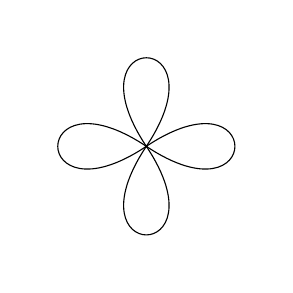
\begin{tikzpicture}[baseline=(current bounding box.center)]
		\draw (0,0) .. controls (1, 1.5) and (-1, 1.5) .. (0,0);
		\draw[rotate=90] (0,0) .. controls (1, 1.5) and (-1, 1.5) .. (0,0);
		\draw[rotate=180] (0,0) .. controls (1, 1.5) and (-1, 1.5) .. (0,0);
		\draw[rotate=270] (0,0) .. controls (1, 1.5) and (-1, 1.5) .. (0,0);
	\end{tikzpicture}\]
	我们断言存在群同构 $\mathbf{F}(X) \rightiso \pi_1(B_X, \star)$, 它将 $x \in X$ 映至 $B_X$ 中从 $\star$ 出发, 沿第 $x$ 份 $\mathbb{S}^1$ 顺向绕一圈的道路. 当 $|X|=1$ 时这无非是习见的同构 $\pi_1(\mathbb{S}^1, \star) \rightiso \Z$ \cite[第四章 \S 3.1]{You}. 一般情形则从 van Kampen 定理导出, 其有限版本可见 \cite[附录B]{You}.

	回顾图的概念. 一个图 $\Gamma = (V, E, s, t)$ 是由顶点集 $V$ 和边集 $E$ 组成的, 边有头尾两端, 由一对映射 $s, t: E \to V$ 给出. 从 $\Gamma$ 可以构造其几何实现 $|\Gamma|$: 说穿了, 这无非是对每个边具体地取一份区间 $[0, 1]$, 并沿顶点黏合成 $|\Gamma|$. 以下等同 $\Gamma$ 与 $|\Gamma|$, 所论的图因之是无向的. 先前定义的 $B_X$ 就是仅有一个顶点的图. 图论的一个基本结果断言当 $\Gamma$ 连通时, 必存在极大子树 $T$: 它是 $\Gamma$ 的子图, 包含 $\Gamma$ 的每个顶点并且不含回路. 直观地看, 我们可以在 $\Gamma$ 中让树 $T$ 连续地收缩到某顶点 $\star$ (这称为形变收缩, 见 \cite[第四章 \S 4.3]{You}); 譬如在下图中缩掉粗线标出的极大子树, 就得到之前的四叶幸运草.
	\begin{center}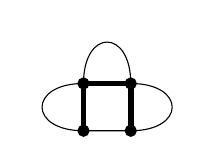
\begin{tikzpicture}[every node/.style={circle, draw, fill=black}, bentcurve/.style={bend left=90, looseness=3} ]
		\begin{scope}[scale=0.6]
			\coordinate (A) at (0,0) {};
			\coordinate (B) at (0,1) {};
			\coordinate (C) at (1,1) {};
			\coordinate (D) at (1, 0) {};
		\end{scope}
		\draw [line width=2pt] (A) -- (B) -- (C) -- (D);
		\draw[bentcurve] (A) to (B) to (C) to (D) --cycle;
		\foreach \x in {A, B, C, D}
			\draw[circle, fill=black] (\x) circle[radius=2pt];
	\end{tikzpicture}\end{center}
	一般情形下, 因 $T$ 含所有顶点, 商空间 $\Gamma/T$ 将同胚于某个 $B_Y$. 故
	\[ \pi_1(\Gamma, \star)  \rightiso \pi_1(\Gamma/T, \star) \simeq \pi_1(B_Y, \star) \; \text{是自由群}. \]
	取定集合 $X$, 复叠空间的理论 \cite[第五章 \S 4]{You} 告诉我们对 $\mathbf{F}(X) \simeq \pi_1(B_X, \star)$ 的任意子群 $H$, 皆存在复叠空间  $\widetilde{B_X} \to B_X$ 使得 $H$ 是单同态 $\pi_1\left( \widetilde{B_X}, \star \right) \to \pi_1(B_X, \star)$ 的像. 至此, 我们只消证明 $\pi_1\left(\widetilde{B_X}, \star\right)$ 自由; 断言归结为以下性质:
	\begin{center} 图的复叠空间仍为图. \end{center}
	这是复叠空间的道路提升性质的直接推论.
\end{proof}

\section{对称群}\label{sec:symmetric-group}
对集合 $X$, 其\emph{对称群} $\mathfrak{S}_X$ 是全体双射 $X \xrightarrow{1:1} X$ 对映射合成所构成的群, 它自然地左作用于 $X$ 上, 其中元素也称为置换. 本节仅关心 $n := |X|$ 有限的情形, 此时 $|\mathfrak{S}_X| = n!$. 习惯上经常将 $X$ 的元素等同于 $\{1, \ldots, n\}$ 并记 $\mathfrak{S}_n := \mathfrak{S}_{\{1, \ldots, n\}}$. 

对集合 $X$, $Y$ 存在自然的群嵌入 $\mathfrak{S}_X \times \mathfrak{S}_Y \hookrightarrow \mathfrak{S}_{X \sqcup Y}$, 或记作 $\mathfrak{S}_n \times \mathfrak{S}_m \hookrightarrow \mathfrak{S}_{n+m}$. 这里 $\mathfrak{S}_X$ 和 $\mathfrak{S}_Y$ 在 $\mathfrak{S}_{X \sqcup Y}$ 中之所以对乘法交换, 是因为它们所挪动的元素``不交''. 这自然地导向下述定义.

\begin{definition}\index{duichengqun}\index{xunhuan@循环 (cycle)}\index{duihuan@对换 (transposition)} \index[sym1]{S_n@$\mathfrak{S}_n$}
	设 $a_1, \ldots, a_m$ 是 $X$ 中相异的元素. 对称群 $\mathfrak{S}_X$ 中的 $m$-\emph{循环} (又称轮换) $(a_1 \cdots a_m)$ 是下述映射 $\sigma: X \to X$
	\begin{gather*}
		\sigma(a_i) = a_{i+1}, \quad i \in \Z/m\Z, \\
		\sigma(x)=x, \quad x \notin \{a_1, \ldots, a_m\},
	\end{gather*}
	在此将下标 $\{1, \ldots, m\}$ 方便地视为 $\Z/m\Z$ 中元素, 即模 $m$ 的同余类. 称 $m$ 为该循环的长度; $2$-循环 $(a b)$ 又称\emph{对换}. 我们称 $\mathfrak{S}_X$ 中两个循环 $(a_1 \cdots a_m)$, $(b_1 \cdots b_k)$ 不交, 如果 $\{a_1, \ldots, a_m\} \cap \{b_1, \ldots, b_k\} = \emptyset$. 
\end{definition}
由先前讨论可知不交的循环对乘法相交换. 同样显然的是 $\text{ord}((a_1 \cdots a_m)) = m$.

\begin{proposition}[循环分解]\label{prop:cyclic-decomposition}
	每个 $\sigma \in \mathfrak{S}_X$ 都能表成不交的循环之积
	\[ \sigma = (a_1 a_2 \cdots) (b_1 b_2 \cdots) \cdots \]
	其中的循环 $(a_1 \cdots)$, $(b_1 \cdots)$ 在至多差一个顺序的意义下唯一. 由于 $1$-循环是单位元, 乘积中可以省去.
\end{proposition}
\begin{proof}
	这无非是 $X$ 在 $\sigma$ 生成的有限循环群 $\lrangle{\sigma}$ 下的轨道分解 (引理 \ref{prop:orbit-decomp}), 每个循环对应到一个轨道, 描述了 $\sigma$ 在该轨道上的作用.
\end{proof}

我们称循环分解中出现的循环长度 $n_1, n_2, \ldots$ (包括长度为一的循环) 为 $\sigma$ 的循环型, 计重数不计顺序. 为了得到唯一性, 不妨排成 $n_1 \geq n_2 \geq \cdots$, 循环型因之对应于整数 $n := |X|$ 的分拆: $n = n_1 + n_2 + \cdots$. 上面对阶数的讨论蕴涵 $\sigma$ 的阶数等于 $n_1, n_2, \ldots$ 的最小公倍数. \index{fenchai@分拆 (partition)}

据此, 共轭作用在对称群情形下有干净的陈述.
\begin{lemma}\label{prop:cycle-type}
	设 $\tau = (a_1 a_2 \cdots) (b_1 \cdots) \cdots$ 为上述的循环分解, $\tau \in \mathfrak{S}_X$, 则
	\[ \sigma \tau \sigma^{-1} = (\sigma(a_1) \sigma(a_2) \cdots) (\sigma(b_1) \cdots) \cdots. \]
	作为推论, 元素 $\tau$ 的共轭类由其循环型确定; $\mathfrak{S}_X$ 中的共轭类一一对应于循环型 $n_1 \geq n_2 \geq \cdots$, 后者又一一对应于整数 $n = |X|$ 的分拆.
\end{lemma}
\begin{proof}
	易见 $\sigma \tau \sigma^{-1}$ 将 $\sigma(a_i)$ 映至 $\sigma(a_{i+1})$, 将 $\sigma(b_j)$ 映至 $\sigma(b_{j+1})$, 依此类推. 由于 $\sigma$ 是双射, 由此唯一确定了 $\sigma \tau \sigma^{-1}$ 的循环分解. 适当选取 $\sigma$ 即可使 $\sigma\tau\sigma^{-1}$ 成为任意与 $\tau$ 有同样循环型的元素, 证毕. 
\end{proof}

下面我们改采符号 $\mathfrak{S}_n$.
\begin{lemma}\label{prop:S_n-generation}
	群 $\mathfrak{S}_n$ 由对换 $\tau_i = (i \quad i+1)$ 生成, 这里 $1 \leq i < n$.
\end{lemma}
\begin{proof}
	将给定的置换 $\sigma$ 视同数列 $\sigma(1), \ldots, \sigma(n)$, 则表 $\sigma$ 为诸 $\tau_i$ 的积相当于借由反复交换数列中的相邻项, 将 $\sigma(1), \ldots, \sigma(n)$ 逐步化成 $1, \ldots, n$; 这当然是可行的. 严格论证留给有闲情逸致的读者.
\end{proof}

\begin{lemma}\index[sym1]{sgn@$\sgn$}
	存在唯一的群同态 $\sgn: \mathfrak{S}_n \to \{\pm 1\}$ 使得 $\sgn((a_1 \cdots a_m)) = (-1)^{m+1}$.
\end{lemma}
\begin{proof}
	群 $\mathfrak{S}_n$ 在函数集 $\{ f: \Z^n \to \Z\}$ 上有自然的左作用
	\[ (\sigma f)(x_1, \ldots, x_n) = f(x_{\sigma(1)}, \ldots, x_{\sigma(n)}), \]
	此作用对函数的逐点加法显然为线性: $\sigma(f \pm g) = \sigma f \pm \sigma g$, 其中 $k \in \Z$. 今考虑函数
	\[ \Delta(x_1, \ldots, x_n) = \prod_{1 \leq i < j \leq n} (x_j - x_i). \]
	对于 $\sigma \in \mathfrak{S}_n$, 显见存在 $\sgn(\sigma) \in \{\pm 1\}$ 使得 $\sigma \Delta = \sgn(\sigma)\Delta$. 因为 $\Delta$ 不恒为零 (代入 $x_i = i$ 可知), $\sgn(\sigma)$ 是唯一确定的, 因而 $\sgn: \mathfrak{S}_n \to \{\pm1 \}$ 是群同态. 容易验证对每个 $1 \leq i < n$ 皆有 $\tau_i \Delta = -\Delta$. 对换之间两两共轭, 故对所有对换 $\tau \in \mathfrak{S}_n$ 皆有 $\sgn(\tau)=-1$. 由
	\[(a_1 \cdots a_m) = (a_1 a_m) (a_1 \cdots a_{m-1}) = \cdots = (a_1 a_m) (a_1 a_{m-1}) \cdots (a_1 a_2) \]
	可见 $\sgn((a_1 \cdots a_m)) = (-1)^{m+1}$. 唯一性导自命题 \ref{prop:cyclic-decomposition}. 
\end{proof}

\begin{definition}[交错群]\index[sym1]{A_n@$\mathfrak{A}_n$}
	定义\emph{交错群} $\mathfrak{A}_n$ 为 $\Ker[ \mathfrak{S}_n \xrightarrow{\sgn} \{\pm 1\}]$, 它是 $\mathfrak{S}_n$ 的正规子群.
\end{definition}
落在 $\mathfrak{A}_n$ 中的置换称为偶置换, 否则称为奇置换. 当 $n > 1$ 时 $(\mathfrak{S}_n : \mathfrak{A}_n) = |\{\pm 1\}| = 2$. 当 $n \geq 4$ 时 $\mathfrak{A}_n$ 非交换, 例如: $(1 2 3)(1 2 4) = (1 3) (2 4)$ 而 $(1 2 4)(1 2 3) = (1 4) (2 3)$.

我们需要以下简单的性质:
\begin{itemize}
	\item 群 $\mathfrak{S}_n$ 的导出子群 (见 \S\ref{sec:solvable-groups}) $\mathscr{D}^1 \mathfrak{S}_n$ 等于 $\mathfrak{A}_n$. 当 $n=1$ 时此为显然. 以下解释 $n \geq 2$ 情形: $\mathfrak{S}_n$ 由对换生成, 每个对换都共轭于 $(1 \; 2)$, 故交换商 $\mathfrak{S}_n / \mathscr{D}^1 \mathfrak{S}_n$ 由 $(1 \; 2)$ 的像生成, 这是二阶元. 另一方面引理 \ref{prop:abelianization} 给出满同态
		\[ \mathfrak{S}_n / \mathscr{D}^1 \mathfrak{S}_n \stackrel{\text{商同态}}{\twoheadrightarrow} \mathfrak{S}_n/\mathfrak{A}_n \simeq \{ \pm 1\}. \]
		比较阶数可见以上同态实为同构, 亦即 $\mathscr{D}^1 \mathfrak{S}_n = \mathfrak{A}_n$.
	\item 所有 $\mathfrak{S}_n$ 中长度为奇数的循环皆包含于 $\mathfrak{A}_n$.
	\item 当 $n \geq 3$ 时, $\mathfrak{A}_n$ 由 $3$-循环 (形如 $(i j k)$) 生成. 这是由于任意 $\sigma \in \mathfrak{A}_n$ 可以表成对换的积, $\sgn(\sigma)=1$ 确保乘积有偶数个项. 运用以下观察
		\[ (i j)(k l) = \begin{cases}
			1, & \{i,j\} = \{k,l\}, \\
			\text{$3$-循环}, & \{i,j\} \cap \ \{k,l\}\; \text{恰有一元素}, \\
			(i j k) (j k l), & \{i,j\} \cap \ \{k,l\} = \emptyset
		\end{cases} \]
		可将乘积改写为 $3$-循环的积.
	\item 当 $n \geq 5$ 时, 任两个 $3$-循环 $(i j k)$, $(i' j' k')$ 在 $\mathfrak{A}_n$ 中共轭. 首先留意到引理 \ref{prop:cycle-type} 蕴涵存在 $\sigma \in \mathfrak{S}_n$ 使得 $\sigma (i j k) \sigma^{-1} = (i' j' k')$. 若 $\sigma \in \mathfrak{A}_n$ 则收工, 否则取相异元 $l, m \in \{1, \ldots, n\} \smallsetminus \{i,j,k\}$ 并置 $\sigma' := \sigma \cdot (l m) \in \mathfrak{A}_n$; 对之仍有 $\sigma' (i j k) (\sigma')^{-1} = (i' j' k')$.
\end{itemize}
以下记任意置换 $\sigma$ 的不动点集为 $\text{Fix}(\sigma) := \left\{ i: \sigma(i)=i \right\}$.

\begin{theorem}[É.\ Galois]\label{prop:A_n-simple}
	当 $n \geq 5$ 时 $\mathfrak{A}_n$ 是单群.
\end{theorem}
\begin{proof}
	设 $H \lhd \mathfrak{A}_n$, $H \neq \{1\}$. 从以上性质可知找出一个 $3$-循环 $\sigma \in H$ 即足. 兹断言取 $\sigma \in H \smallsetminus \{1\}$ 使得 $\left|\text{Fix}(\sigma)\right|$ 极大便是.
	
	如果 $\sigma$ 的循环分解中只有对换, 那么分解中至少含两项如 $(i j) (k l)$, 其中 $\{i,j\} \cap \{k,l\} = \emptyset$. 由于 $n \geq 5$, 可取 $r \notin \{i,j,k, l\}$ 并定义
	\begin{equation}\label{eqn:tau-sigma-simple}
		\tau := (k l r), \quad \sigma' := [\tau, \sigma] = \tau\sigma\tau^{-1}\sigma^{-1} \in H \quad (\because H \lhd \mathfrak{A}_n).
	\end{equation}
	可直接验证 $i,j \in \text{Fix}(\sigma') \smallsetminus \text{Fix}(\sigma)$, $\sigma'(k) = r \neq k$, 以及
	\[ \text{Fix}(\sigma) \smallsetminus \{r\} = \text{Fix}(\sigma) \smallsetminus \{k, l, r\} = \text{Fix}(\sigma) \cap \text{Fix}(\tau) \subset \text{Fix}(\sigma'). \]
	综之 $\left|\text{Fix}(\sigma')\right| > \left|\mathrm{Fix}(\sigma)\right|$, 矛盾.
	
	设 $\sigma$ 的循环分解中包含长度 $>2$ 的项 $(i j k \cdots)$. 假若 $\sigma = (i j k)$ 则是所求的 $3$-循环; 否则因为 $\sigma$ 不可能是 $4$-循环, $\sigma$ 除了 $i,j,k$ 之外还挪动至少两个相异元 $r, l$. 依然以 \eqref{eqn:tau-sigma-simple} 式定义 $\sigma' \in H$. 可以验证 $j \in \text{Fix}(\sigma')$, $\sigma'(k) = l \neq k$ 和
	\[ \text{Fix}(\sigma) = \text{Fix}(\sigma) \smallsetminus \{k,l,r\} = \text{Fix}(\sigma) \cap \text{Fix}(\tau) \subset \text{Fix}(\sigma'). \]
	仍得到矛盾 $\left|\text{Fix}(\sigma')\right| > \left|\mathrm{Fix}(\sigma)\right|$. 明所欲证.
\end{proof}

当 $n \geq 5$ 时 $\mathfrak{A}_n$ 是非交换单群, 因此它必然等于自身的导出子群 $\mathscr{D}^1 \mathfrak{A}_n$. 下述推论是证明五次以上方程无根式解 (定理 \ref{prop:Abel-Ruffini}) 的群论钥匙.
\begin{corollary}\label{prop:S_n-unsolvable}\index{kejiequn}
	当 $n \geq 5$ 时, 对所有 $i \geq 1$ 都有 $\mathscr{D}^i \mathfrak{S}_n = \mathfrak{A}_n$; 作为推论, 当 $n \geq 5$ 时 $\mathfrak{S}_n$ 不可解.
\end{corollary}
\begin{proof}
	已知 $\mathscr{D}^1 \mathfrak{S}_n = \mathfrak{A}_n$. 配合前述讨论, 当 $n \geq 5$ 时, 对所有 $i \geq 1$ 皆有 $\mathscr{D}^i \mathfrak{S}_n = \mathscr{D}^{i-1} \mathfrak{A}_n = \mathfrak{A}_n$. 关于不可解性的断言请见引理 \ref{prop:solvable-nilpotent-characterization}.
\end{proof}

读者可以动手验证 $\mathscr{D}^1 \mathfrak{A}_4 = \left\{\identity, (1 2)(3 4), (1 3) (2 4), (1 4)(2 3)\right\}$, 同构于 $(\Z/2\Z)^2$. 因此 $n < 5$ 时 $\mathfrak{S}_n$ 确实可解.

我们接着考察 $\mathfrak{S}_n$ 的展示. 为此不妨一并考虑例 \ref{eg:braid} 提到的辫群 $\mathcal{B}_n$. 简要摘录之前的构造如下: 形象地看, $\mathcal{B}_n$ 是由所有 $n$ 条线编成的辫子为元素的群, 辫子在空间 $\R^3$ 中连续的形变下 (不动端点, 不割断线) 视为等价. 辫子可以图解为诸如 ($n=2,3$)
\begin{center}\begin{tikzpicture}[baseline=(braid)]
	\braid[style strands={1}, style strands={2}] (braid) s_1;
	\end{tikzpicture} \qquad \begin{tikzpicture}[baseline=(braid), yscale=0.8]
	\braid[style strands={1}, style strands={2}, style strands={3}] (braid)  s_1 s_2^{-1};
\end{tikzpicture}\end{center}
的形式. 辫群中的乘法是将辫子从上而下地接合, 如
\begin{center}\begin{tikzpicture}[baseline=(braid)]
	\braid[style strands={1}, style strands={2}] (braid) s_1;
	\end{tikzpicture} \quad $\bullet$ \quad \begin{tikzpicture}[baseline=(braid)]
	\braid[style strands={1}, style strands={2}] (braid) s_1^{-1};
	\end{tikzpicture} \quad $=$ \quad \begin{tikzpicture}[baseline=(braid), yscale=0.8]
	\braid[style strands={1}, style strands={2}] (braid) s_1 s_1^{-1};
	\end{tikzpicture} \quad $\xlongequal{\text{拉直}}$ \quad
	\begin{tikzpicture}[baseline=(M), yscale=0.8]
	\draw (0,1) -- (0,-1);
	\draw (1,1) -- (1,-1);
	\coordinate (M) at (0,0);
\end{tikzpicture}\end{center}
结合律一望可知, $\mathcal{B}_n$ 的幺元是 $n$ 条平行线 $\vert \cdots \vert$. 辫子的图表对水平轴作镜射给出其逆, 何以故? 请端详上图.

两组辫子的``横向并列''导出群同态 $\mathcal{B}_n \times \mathcal{B}_m \to \mathcal{B}_{n+m}$.

显然 $\mathcal{B}_1 = \{1\}$. 以下假设 $n \geq 2$. 对 $1 \leq i < n$, 定义元素 $\sigma_i \in \mathcal{B}_n$ 使得其中第 $i$, $i+1$ 条线的缠绕模式为
\begin{center} \begin{tikzpicture}
	\braid[style strands={1}, style strands={2}] (braid) s_1;
	\node[above] at (braid-1-s) {$i$};
	\node[above] at (braid-2-s) {$i+1$};
\end{tikzpicture} \end{center}
其余诸线则不相缠绕. 容易看出当 $|i-j| > 1$ 时, $\sigma_i$, $\sigma_j$ 影响的线不交故 $\sigma_i \sigma_j = \sigma_j \sigma_i$; 另一方面, ``杨--Baxter 方程''
\[ \begin{tikzpicture}[yscale=0.6, baseline=(braid)]
	\braid[style strands={1}, style strands={2}, style strands={3}] (braid) s_1 s_2 s_1;
	\node[above] at (braid-1-s) {$i$};
	\node[above] at (braid-2-s) {$i+1$};
	\node[above] at (braid-3-s) {$i+2$};
	\end{tikzpicture}
	\qquad = \qquad
	\begin{tikzpicture}[yscale=0.6, baseline=(braid)]
	\braid[style strands={1}, style strands={2}, style strands={3}] (braid) s_2 s_1 s_2;
	\node[above] at (braid-1-s) {$i$};
	\node[above] at (braid-2-s) {$i+1$};
	\node[above] at (braid-3-s) {$i+2$};
\end{tikzpicture} \]
表明 $\sigma_i \sigma_{i+1} \sigma_i = \sigma_{i+1} \sigma_i \sigma_{i+1}$ 对 $1 \leq i < n-1$ 恒成立. 请读者试着直观地理解
\begin{inparaenum}[(a)]
	\item 元素 $\sigma_1, \ldots, \sigma_{n-1}$ 生成 $\mathcal{B}_n$,
	\item 关系式 $|i-j| > 1 \implies \sigma_i \sigma_j = \sigma_j \sigma_i$ 和 $\sigma_i \sigma_{i+1} \sigma_i = \sigma_{i+1} \sigma_i \sigma_{i+1}$ 完全描述了 $\mathcal{B}_n$ 的结构.
\end{inparaenum}
更精简的说法是借助群的展示
\begin{equation}\label{eqn:braid-presentation} \left\langle \sigma_1, \ldots, \sigma_{n-1} \Biggr| \begin{array}{ll}
	\sigma_i \sigma_j = \sigma_j \sigma_i, & |i-j| > 1 \\
	\sigma_i \sigma_{i+1} \sigma_i = \sigma_{i+1} \sigma_i \sigma_{i+1}, & 1 \leq i < n-1
	\end{array} \right\rangle \rightiso \mathcal{B}_n. \end{equation}

这个展示既可以从 $\mathcal{B}_n$ 的拓扑诠释推导, 亦可直接当作辫群的组合学定义. 留意到 $\mathcal{B}_2 \simeq \Z$, 当 $n \geq 3$ 时 $\mathcal{B}_n$ 是无穷非交换群.

现在我们来联系 $\mathcal{B}_n$ 与 $\mathfrak{S}_n$. 对每条辫子 $x \in \mathcal{B}_n$, 定义相应的 $\sigma \in \mathfrak{S}_n$ 使得辫图从底端 $i$ 走到顶端 $\sigma(i)$ 如下
\begin{center}\begin{tikzpicture}[scale=0.5]
	\node (S) at (-1.7, 1) {$\sigma(i)$};
	\node (E) at (1.7, -1) {$i$};
	\draw (S) -- (E) node[midway, fill=white, anchor=center, sloped] {$\cdots$};
\end{tikzpicture}\end{center}
易见这给出群同态 $\mathcal{B}_n \to \mathfrak{S}_n$, 它使图表
\[\begin{tikzcd}
	\mathcal{B}_n \times \mathcal{B}_m \arrow[r] \arrow[d] & \mathcal{B}_{n+m} \arrow[d] \\
	\mathfrak{S}_n \times \mathfrak{S}_m \arrow[r] & \mathfrak{S}_{n+m}
\end{tikzcd}\]
交换, 并将 $\sigma_i \in \mathcal{B}_n$ 映到对换
\[ \tau_i := (i \quad i+1) \in \mathfrak{S}_n, \quad 1 \leq i < n. \]
引理 \ref{prop:S_n-generation} 断言它们生成 $\mathfrak{S}_n$. 如改从 $\mathcal{B}_n$ 的展示 \eqref{eqn:braid-presentation} 切入, 我们可以先在 $\mathfrak{S}_n$ 中验证关系式
\begin{gather*}
	|i-j| > 1 \implies \tau_i \tau_j = \tau_j \tau_i, \\
	\tau_i^2 = 1, \quad 1 \leq i < n, \\
	\tau_i \tau_{i+1} \tau_i = \tau_{i+1} \tau_i \tau_{i+1} = (i \quad i+2), \quad 1 \leq i < n-1.
\end{gather*}
所以 $\sigma_i \mapsto \tau_i$ 确定了同态 $\mathcal{B}_n \to \mathfrak{S}_n$. 这就引出一个显然的问题: 这些关系式是否给出 $\mathfrak{S}_n$ 的展示?

为避免歧义, 另立符号 $\tilde{\tau}_i$ 代入以上三族关系式, 联立后能够化作等价形式
\begin{equation}\label{eqn:S_n-presentation}\begin{gathered}
	\tilde{\tau}_i^2 = 1, \quad 1 \leq i < n \\
	|i-j| > 1 \implies (\tilde{\tau}_i \tilde{\tau}_j)^2 = 1, \\
	(\tilde{\tau}_i \tilde{\tau}_{i+1})^3 = 1, \quad 1 \leq i < n-1.
\end{gathered}\end{equation}
定义 $\mathfrak{S}'_n := \lrangle{\tilde{\tau}_1, \ldots, \tilde{\tau}_n \big| \text{满足于}\; \eqref{eqn:S_n-presentation} }$, 另外约定 $\mathfrak{S}'_1 := \{1\}$. 因之有群同态 $\mathcal{B}_n \twoheadrightarrow \mathfrak{S}'_n \twoheadrightarrow \mathfrak{S}_n$, 满足 $\sigma_i \mapsto \tilde{\tau}_i \mapsto \tau_i$. 从 $\mathcal{B}_n$ 过渡到 $\mathfrak{S}'_n$ 相当于忽视缠绕
\begin{tikzpicture}[baseline=(braid), yscale=0.5, xscale=0.7]
	\braid[style strands={1}, style strands={2}] (braid) s_1 s_1;
\end{tikzpicture}.

\begin{theorem}\label{prop:S_n-presentation}
	映射 $\mathfrak{S}'_n \to \mathfrak{S}_n$ 是同构, 换言之 \eqref{eqn:S_n-presentation} 确实给出 $\mathfrak{S}_n$ 的展示.
\end{theorem}
\begin{proof}
	既然 $\mathfrak{S}'_n \to \mathfrak{S}_n$ 是满同态, 只要递归地证明 $|\mathfrak{S}'_n| \leq n!$ 即可. 因 $n=1,2$ 的情形是平凡的, 以下设 $n > 2$. 展示 \eqref{eqn:S_n-presentation} 给出自然同态 $\mathfrak{S}'_{n-1} \to \mathfrak{S}'_n$. 我们暂不知这是否为单射, 但总能让 $\mathfrak{S}'_{n-1}$ 以右乘作用在 $\mathfrak{S}'_n$ 上并考察其轨道. 今断言
	\[ \mathfrak{S}'_n = 1 \cdot \mathfrak{S}'_{n-1} \cup \tilde{\tau}_{n-1}\mathfrak{S}'_{n-1} \cup \cdots \cup (\tilde{\tau}_1 \cdots \tilde{\tau}_{n-1} \mathfrak{S}'_{n-1}), \]
	若此式成立, 立得 $\mathfrak{S}'_n \leq n |\mathfrak{S}'_{n-1}| \leq n(n-1)! = n!$.
	
	仅须证明等式右侧在每个 $\tilde{\tau}_i$ 的左乘下保持封闭. 考虑 $\tilde{\tau}_i (\tilde{\tau}_j \cdots \tilde{\tau}_{n-1}) \mathfrak{S}'_{n-1}$: 当 $i=j-1$ 或 $i=j$ 时显然有封闭性 ($\tilde{\tau}_j^2 = 1$); 当 $i < j-1$ 时用 \eqref{eqn:S_n-presentation} 可将 $\tilde{\tau}_i$ 朝右吸收到 $\mathfrak{S}'_{n-1}$, 依然封闭. 故以下假设 $i>j$. 我们利用 \eqref{eqn:S_n-presentation} 的第二式将 $\bm{\tilde{\tau}_i}$ 右移 (为强调故变化字体), 直到
	\[ \cdots \tilde{\tau}_{i-2} \bm{\tilde{\tau}_i} \tilde{\tau}_{i-1} \tilde{\tau}_i \tilde{\tau}_{i+1} \cdots \mathfrak{S}'_{n-1}. \]
	接着应用 \eqref{eqn:S_n-presentation} 的第三式 (或它在 \eqref{eqn:braid-presentation} 中的形式) 化之为
	\[ \cdots \tilde{\tau}_{i-2} \tilde{\tau}_{i-1} \tilde{\tau}_i \bm{\tilde{\tau}_{i-1}} \tilde{\tau}_{i+1} \cdots \mathfrak{S}'_{n-1}. \]
	上式标出的 $\bm{\tilde{\tau}_{i-1}}$ 可一路右移直到并入 $\mathfrak{S}'_{n-1}$, 故所求的左乘封闭性成立.
\end{proof}

展示 \eqref{eqn:S_n-presentation} 表明对称群属于一类称为 Coxeter 群的构造, 它们带有形如 $W = \lrangle{S \big| (st)^{m(s,t)}=1, \; s,t \in S}$ 的展示, 其中
\begin{compactitem}
	\item $S$ 是有限集,
	\item $m: S \times S \to \Z_{\geq 1} \sqcup \{\infty\}$ (取 $\infty$ 意谓无关系),
	\item $\forall s,t \in S, \; m(s,t)=m(t,s)$,
	\item $s=t \iff m(s,t)=1$.
\end{compactitem}
例 \ref{eg:dihedral-presentation} 表明二面体群 $D_{2n}$ 也具有这种展示. Coxeter 群是研究 Lie 群, Lie 代数和相关表示理论的必备工具. \index{Coxeter 群}

\section{群的极限和完备化}\label{sec:group-limit}
基于 \S\ref{sec:free-group} 的构造和例 \ref{eg:complete-cocomplete}, 群范畴 $\cate{Grp}$ 和其子范畴 $\cate{Ab}$ 中可以定义极限 $\varinjlim$ 和 $\varprojlim$. 构造方法已在例 \ref{eg:complete-cocomplete} 大致说明. 本节将深入探讨 $\varprojlim$ 的情形.

对于小范畴 $I$, 给定函子 $\beta: I^\text{op} \to \cate{Grp}$ 相当于给定一族群 $\{ G_i := \beta(i) : i \in \Obj(I) \}$, 并对每个箭头 $s: i \to j$ 指定群同态 $\beta(s): G_j \to G_i$, 使得
\begin{compactitem}
	\item $\beta(\identity: i \to i)=\identity_{G_i}$,
	\item 合成箭头 $i \to j \to k$ 给出合成同态 $G_k \to G_j \to G_i$.
\end{compactitem}
例 \ref{eg:complete-cocomplete} 已将 $\varprojlim_i G_i := \varprojlim \beta$ 的存在性归结为积和等化子的存在性. 铺开定理 \ref{prop:limit-buildingblocks} 证明中的构造, 便得到明白的表法
\[
	\varprojlim_i G_i := \left\{ (x_i)_{i \in I} \in \prod_{i \in I} G_i : \forall s: i \to j, \; \beta(s)(x_j) = x_i \right\}.
\]
显然 $\varprojlim_i G_i$ 构成直积 $\prod_{i \in I} G_i$ 的子群. 同时我们也得到自明的投影同态 $p_j: \varprojlim_i G_i \to G_j$.

以下将假设 $I$ 实由偏序集 $(I, \leq)$ 给出 (参看例 \ref{eg:categories}); 并且 $(I, \leq)$ 是\emph{滤过}的, 即任意两元素都有共同上界 (定义 \ref{def:filtrant-poset}). 滤过偏序是滤过范畴的一个特例, 请见定义 \ref{def:filtrant-cat}.\index{luguoxuji}

首先回顾一些点集拓扑学的定义, 详见 \cite[第一章]{FL14}.
\begin{definition}\label{def:topological-group}\index{tuopuqun@拓扑群 (topological group)}
	一个拓扑群 $G$ 意指群 $G$ 上带有拓扑结构, 使得乘法 $m: G \times G \to G$ 与取逆运算 $i: G \to G$ 皆为连续映射.
\end{definition}
典型例子是加法群 $(\R^n, +)$. 作为推论, 任意 $g \in G$ 的左乘或右乘作用都给出同胚 $G \to G$, 取逆亦同. 基于此, 群的拓扑完全由幺元 $1$ 的邻域基反映, 因为总能以左右乘法将基平移到 $G$ 的每一点, 而且 $1$ 的一组邻域基各个取逆后仍是邻域基. 反过来, 给定群 $G$ 的一族子集 $\{H_i \ni 1\}_{i \in I}$, 能否靠左右平移赋予 $G$ 拓扑群结构, 并使该子集给出 $1$ 处的开邻域基? 以下情形对我们已经足够了: 假定 $(I, \leq)$ 是滤过偏序集, $i \leq j \implies H_j \subset H_i$ 而且 $\forall i \; H_i \lhd G$, 那么这样的拓扑总是存在: 事实上
\[ \text{子集}\; E \subset G\; \text{为开} \iff \forall x \in E, \; \exists i \in I, \; xH_i = H_i x \subset E. \]
易见这的确使 $G$ 成拓扑群, 验证留作简单习题. 进一步, 拓扑的分离性公理也简化了.

\begin{lemma}\label{prop:top-group-separation}
	设 $G$ 为拓扑群, 则
	\begin{equation}\label{eqn:top-group-Hausdorff}
		G:\; \text{Hausdorff} \iff \{1\} \subset G\; \text{为闭子集} \iff \bigcap_{U \ni 1: \text{开邻域}} U = \{1\}.
	\end{equation}
	此外, 任何 $x \in G$ 都有一组由闭邻域构成的邻域基.
\end{lemma}
\begin{proof}
	先处理第一条. 对每个 $x \in G$ 置 $\mathfrak{N}_x := \left\{ x \;\text{的所有邻域} \right\}$. 先前关于邻域基的讨论给出 $\mathfrak{N}_x = x\mathfrak{N}_1 = x \mathfrak{N}_1^{-1}$ (意谓对每个邻域都用 $x$ 平移或取逆), 从而
	\begin{equation*}\begin{aligned}
		x \in \overline{\left\{ 1 \right\}} & \iff 1 \in \bigcap_{V \in \mathfrak{N}_x} V = \bigcap_{U \in \mathfrak{N}_1} xU^{-1} \\
		& \iff x^{-1} \in \bigcap_{U \in \mathfrak{N}_1} U^{-1} \iff x \in \bigcap_{U \in \mathfrak{N}_1} U.
	\end{aligned}\end{equation*}
	换言之 $\overline{\{1\}} = \bigcap_{U \in \mathfrak{N}_1} U$. 由之立见第二个 $\iff$. 对第一个 $\iff$ 仅 $\Leftarrow$ 方向非平凡: 定义连续函数 $\nu: G \times G \to G$ 映 $(x,y)$ 为 $xy^{-1}$, 那么 $G$ 是 Hausdorff 空间等价于对角子集 $\Delta_G \subset G \times G$ 为闭, 但 $\Delta_G = \nu^{-1}(1)$ 而 $\{1\} \subset G$ 为闭.

	第二条即刻化约到 $x=1$ 的情形; 由于群运算的连续性, 对任何开邻域 $V \ni 1$ 皆存在开集 $U \ni 1$ 使得 $U^{-1}U \subset V$, 只须观察到闭包 $\bar{U}$ 包含于 $U^{-1} \cdot U$: 这是因为 $g \in \bar{U}$ 蕴涵 $Ug \cap U \neq \emptyset$.
\end{proof}

\begin{lemma}\label{prop:open-closed-subgroup}
	设拓扑群 $G$ 的子群 $H$ 是 $1$ 的邻域, 则 $H$ 既开又闭, 而且 $G$ 紧蕴涵 $(G:H)$ 有限.
\end{lemma}
\begin{proof}
	取开集 $U$ 使得 $1 \in U \subset H$, 因此 $H = \bigcup_{x \in H} Ux$ 为开. 取 $G/H$ 在 $G$ 中的一族代表元 $\Xi$, 则陪集分解 (引理 \ref{prop:coset-decomp}) 给出 $G$ 的开覆盖 $G = \bigsqcup_{x \in \Xi} xH$. 于是 $H = G \smallsetminus \bigsqcup_{\substack{x \in \Xi \\ xH \neq H}} xH$ 为闭, 而且当 $G$ 紧时 $\Xi$ 有限.
\end{proof}

回到 $\varprojlim_i G_i$. 今假设每个 $G_i$ 皆是拓扑群, 且对每个 $i \leq j$ 同态 $G_j \to G_i$ 皆连续. 我们赋 $\prod_{i \in I} G_i$ 予积拓扑 (见 \cite[\S 3.3]{Xiong}), 其子群 $\varprojlim_i G_i$ 遂继承了自然的拓扑群结构.
\begin{lemma}\label{prop:completion-compactness}
	拓扑群 $\varprojlim_i G_i$ 在 $1$ 处有一组形如
	\[ \mathcal{U}_{I_0} = \bigcap_{i \in I_0} p_i^{-1}(U_i), \qquad I_0 \subset I: \; \text{ 有限子集}, \quad U_i \ni 1: \; \text{开子集} \]
	的邻域基. 若每个 $G_i$ 都是 Hausdorff 空间, 则 $\varprojlim_i G_i$ 亦然; 如进一步假设每个 $G_i$ 皆紧, 则 $\varprojlim_i G_i$ 是紧 Hausdorff 空间.
\end{lemma}
由于已设 $(I, \leq)$ 滤过, 描述邻域基时可取 $I_0$ 的上界 $j$, 从而化约到 $I_0 = \{j\}$ 的情形.
\begin{proof}
	邻域基的描述是积拓扑定义的直接推论. Hausdorff 空间的积和子空间仍是 Hausdorff 的, 而 Tychonoff 定理 \cite[定理 7.7.2]{Xiong} 断言紧空间的积仍紧; 从 Hausdorff 性质可推出 $\varprojlim_i G_i$ 是 $\prod_i G_i$ 的闭子群 (它由一族连续函数的等式定义), 故紧.
\end{proof}

在代数及数论中, 较常见的是每个 $G_i$ 皆为有限群的情形, 此时赋予 $G_i$ 离散拓扑使之成为 Hausdorff 紧群.
\begin{definition}[pro-有限群]\label{def:profinite-group}\index{pro-youxianqun@pro-有限群 (pro-finite group)}
	同构意义下形如 $\varprojlim_i G_i$, 其中 $(I, \leq)$ 滤过而且每个 $G_i$ 皆有限的拓扑群, 称作 \emph{pro-有限群}.
\end{definition}

\begin{theorem}\label{prop:profinite-characterization}
	一个拓扑群 $G$ 是 pro-有限群当且仅当它是 Hausdorff 紧群, 而且 $1$ 处有一组由正规子群构成的邻域基.
\end{theorem}
\begin{proof}
	假设 $G = \varprojlim_i G_i$ 为 pro-有限. 我们业已说明 $G$ 为 Hausdorff 紧群. 引理 \ref{prop:completion-compactness} 中的 $U_i$ 可取为 $\{1\}$, 从而 $1$ 的邻域基由一族正规开子群 $U$ 组成.

	现假设拓扑群 $G$ 满足所示条件, 取一组正规子群构成的邻域基, 记为 $I$; 集合的包含关系使 $I$ 成为偏序集, 邻域基的性质确保 $(I, \leq)$ 滤过. 将对应于 $i \in I$ 的正规子群记为 $N_i$. 引理 \ref{prop:open-closed-subgroup} 蕴涵 $G/N_i$ 有限, $N_i$ 既开且闭.

	根据泛性质, 全体商映射 $q_i: G \to G/N_i$ 确定了同态 $\varphi: G \to \varprojlim_i G/N_i$. 我们断言 $\varphi$ 是拓扑群的同构. 首先, 不难验证 $\varphi$ 连续, 而且 Hausdorff 性质确保 $\Ker(\varphi) = \bigcap_{i \in I} N_i = \{1\}$, 故 $\varphi$ 为单射. 今断言 $\Image(\varphi)$ 在 $\varprojlim_i G/N_i$ 中稠密. 诚然, 取 $x = (x_i)_i \in \varprojlim_i G/N_i$, 对任意有限子集 $I_0 \subset I$, 仅需说明 $x^{-1} \Image(\varphi)$ 交 $\bigcap_{i \in I_0} \Ker(p_i)$. 根据滤过偏序集的定义 , 存在 $I_0$ 的一个上界 $k \in I$; 取 $y \in G$ 使得 $q_k(y) = x_k$, 那么对每个 $i \in I_0$ 都会有 $q_i(y) = x_i$, 因而 $x^{-1} \varphi(y) \in \bigcap_{i \in I_0} \Ker(p_i)$.

	由于 $G$ 和 $\varprojlim_i G/N_i$ 都是紧 Hausdorff 空间, 综上 $\varphi$ 自动成为同胚 (见 \cite[\S 7.2]{Xiong}). 明所欲证.
\end{proof}
\begin{remark}\label{rem:totally-disconnected}
	以上条件可以化成更有拓扑味儿的形式: $G$ 为 pro-有限当且仅当 $G$ 是完全不连通的紧群. 证明见 \cite[命题 1.9.3]{FL14}.
\end{remark}

\begin{definition}[群的完备化]\label{def:group-completion} \index{wanbeihua@完备化 (completion)}
	设 $G$ 为群. 假设偏序集 $(I, \leq)$ 滤过. 对每个 $i \in \Obj(I)$ 取定正规子群 $H_i \lhd G$, 并假设 $i \leq j \implies H_j \subset H_i$. 则在 $\varprojlim$ 的定义中可取 $G_i := G/H_i$, 而且 $i \leq j$ (即 $i \to j$) 给出商同态 $G/H_j \twoheadrightarrow G/H_i$. 极限 $\varprojlim_i G/H_i$ 称作 $G$ 对子群族 $(H_i)_{i \in I}$ 的\emph{完备化}.
\end{definition}
完备化带有显然的同态 $\iota: G \xrightarrow{g \mapsto (gH_i)_{i \in I}} \varprojlim_i G/H_i$. 以下概略解释``完备化''与拓扑的关联. 简单起见, 今后假定偏序集 $I$ 可数. 读者对于以 Cauchy 列从 $\Q$ 构造 $\R$ 的手法理应有基本的认知.
\begin{definition}
	拓扑群 $G$ 中的点列 $(x_n)_{n \geq 0}$ 称为 \emph{Cauchy 列}, 如果对任意 $1$ 的开邻域 $U$, 存在 $N \geq 0$ 使得 $n, m \geq N \implies x_n x_m^{-1} \in U$. 假定 $G$ 在 $1$ 处有一组可数邻域基, 如果群 $G$ 的每个 Cauchy 序列都收敛, 则称 $G$ 为\emph{完备}的.
\end{definition}

今后总假设有 $1$ 的可数邻域基. 考虑 $G$ 在拓扑意义下的完备化: 这系指一个拓扑群的同态 $\iota: G \to \hat{G}$, 满足下述性质:
\begin{enumerate}[\bfseries {CO}.1]
	\item $\iota: G \to \iota(G) \subset \hat{G}$ 是同胚;
	\item $\iota$ 的像稠密;
	\item $\hat{G}$ 是完备的 Hausdorff 拓扑群.
\end{enumerate}
完备化的构造方式不止一种, 要旨在于性质 \textbf{CO.1} --- \textbf{CO.3} 唯一刻画了 $(\hat{G}, \iota)$, 精确到一个唯一同构; 其证明可以参照大同小异的命题 \ref{prop:completion-ring-characterization}, 或度量空间情形 \cite[\S 8.1]{Xiong}. 如直观地把握, 则这三条性质说明 $\hat{G}$ 中元素可以用 $G$ 中的 Cauchy 列代表, 而且只要 $\hat{x}, \hat{y} \in \hat{G}$ 足够接近, 则 $G$ 中以之为极限的 Cauchy 列 $(x_n)_n$, $(y_n)_n$ 也会足够接近 (当 $n \gg 0$); 于是 $\hat{G}$ 的结构完全被 $G$ 确定. 如此则思过半矣.

\begin{theorem}
	考虑定义 \ref{def:group-completion} 中的资料 $\{ H_i \lhd G \}_{i \in I}$ 并假定 $\bigcap_i H_i = \{1\}$, 赋予 $G$ 以 $\{H_i : i \in I \}$ 为 $1$ 的邻域基之 Hausdorff 拓扑群结构, 并赋予每个 $G/H_i$ 离散拓扑. 进一步设 $I$ 可数, 则 $\iota: G \to \varprojlim_i G/H_i$ 满足 \textbf{CO.1} --- \textbf{CO.3}, 因而也是拓扑意义下的完备化.
\end{theorem}
\begin{proof}
	可数条件蕴涵 $G$ 和 $\hat{G} := \varprojlim_i G/H_i$ 在幺元处确实有可数邻域基. 由 $\Ker(\iota) = \bigcap_i H_i = \{1\}$ 知 $\iota$ 为单. 引理 \ref{prop:completion-compactness} 中 $\hat{G}$ 的邻域基 $\mathcal{U}_j := \{ \hat{y}=(\bar{y}_i)_i \in \hat{G}: i \leq j \implies \bar{y}_i = 1 \}$ 满足 $\iota^{-1}(\mathcal{U}_j) = H_j$, 因此得到 $\iota$ 连续和 \textbf{CO.1}. 至于 \textbf{CO.2}, 对 $\hat{x} = (\bar{x}_i)_i \in \hat{G}$ 和任给之 $j \in I$, 取 $G \ni x_j \mapsto \bar{x}_j$, 则 $\iota(x_j) \in \hat{x}\mathcal{U}_j$, 故 $\iota(G)$ 稠密.
	
	兹确立 \textbf{CO.3}. 对于 $\hat{G}$ 中 Cauchy 列 $(\hat{x}_n)_n$, 对任给之 $j$, 当 $n,m \gg 0$ 时 $\hat{x}_n \hat{x}_m^{-1} \in \mathcal{U}_j$, 故 $\hat{x}_n$ 的 $j$-分量当 $n \gg 0$ 时为常数, 记作 $\bar{x}_j \in G/H_j$. 置 $\hat{x} := (\bar{x}_i)_i \in \hat{G}$ 即为 $(\hat{x}_n)_n$ 的极限.
\end{proof}

\begin{remark}
	若舍去邻域基的可数条件, 则完备性须改以网 (Moore--Smith 收敛性) 或滤子的语言陈述, 我们将在 \S\ref{sec:filters} 引入滤子, 并回头考察 $\iota: G \to \hat{G}$ 的构造.
\end{remark}

\begin{example}[$p$-进数]\label{eg:p-adic}\index[sym1]{Z_p@$\Z_p$}
	取 $I$ 为全序集 $\Z_{\geq 0}$. 对每个 $i \geq 0$ 定义 $H_i := p^{i+1} \Z$. 完备化 $\varprojlim_i \Z/p^{i+1} \Z$ 记作 $\Z_p$, 其元素无非是一族 $(a_i \in \Z/p^{i+1} \Z)_{i \geq 1}$, 满足 $a_{i+1} \mapsto a_i$. 称此为 $p$-进数的加法群; 我们会在 \S\ref{sec:ring-limits} 探讨 $\Z_p$ 上的乘法结构.
\end{example}

\begin{example}[Tate 模]\index{Tate 模}
	设 $A$ 为交换群, $\ell$ 为素数. 仍取 $I = \Z_{\geq 0}$ 如上. 对每个 $N \in \Z$ 置 $A[N] := \Ker[a \mapsto a^N]$, 显然 $N \mid N' \implies A[N] \subset A[N']$; 置 $A[\ell^\infty] := \bigcup_{n \geq 0} A[\ell^n]$. 定义函子 $V: I^\text{op} \to \cate{Ab}$ 为
	\begin{align*}
		V(i) & := A[\ell^\infty], \\
		V(i \to i+1) & := [a \mapsto a^\ell].
	\end{align*}
	置 $V_\ell(A) := \varprojlim_i V(i)$. 其元素 $(a_i \in A[\ell^\infty])_{i \geq 0}$ 须满足 $a_{i+1}^\ell = a_i$. 称此为\emph{有理 Tate 模}. 以同样方式定义一函子 $T: I^\text{op} \to \cate{Ab}$, 但要求 $T(0) = \{1\}$, 得到的极限是
	\[ T_\ell(A) := \varprojlim_i T(i) \subset V_\ell(A), \]
	称为群 $A$ 的 \emph{Tate 模}. 请留意到 $T(i) = A[\ell^i]$.

	举例明之. 取复环面 $E := \CC \big/(\Z \oplus \Z\tau)$ 所成的加法群, 其中 $\text{Im}(\tau) > 0$. 映射 $(a,b) \mapsto a+b\tau$ 导出同构 $(\R/\Z)^2 \rightiso E$, 而 $(\R/\Z)[\ell^i] = \ell^{-i}\Z/\Z$. 易见图表
	\[ \begin{tikzcd}
		a \bmod \Z \arrow[mapsto]{r} \arrow[mapsto, bend right=60]{ddd} \arrow[phantom, d, sloped, "\in" description] & \ell^{i+1}a \bmod \ell^{i+1} \Z \arrow[mapsto, bend left=60]{ddd} \arrow[phantom, d, sloped, "\in" description] \\
		\ell^{-i-1}\Z/\Z \arrow[d, "{\text{乘以} \ell}"'] \arrow[r, "\sim"] & \Z/\ell^{i+1} \Z \arrow[d, "{\text{商}}"] \\
		\ell^{-i}\Z/\Z \arrow[r, "\sim"'] & \Z/\ell^i \Z \\
		\ell a \bmod \Z \arrow[mapsto]{r} \arrow[phantom, u, sloped, "\in" description] & \ell^{i+1} a \bmod \ell^i \Z \arrow[phantom, u, sloped, "\in" description]
	\end{tikzcd} \]
	交换, 故 $T_\ell(E) \simeq \Z_\ell \oplus \Z_\ell$. 令 $\Gamma := \Z \oplus \Z\tau$, 以上论证实则说明了 $T_\ell(E)$ 自然同构于 $\Gamma$ 对 $(\ell^i \Gamma)_{i \geq 0}$ 的完备化.

	当 $\ell$ 取遍所有素数, 不妨设想 $T_\ell(E)$ 代数地``模拟''了定义 $E$ 的格 $\Gamma$, 而后者又是 $E$ 的拓扑不变量 $H_1(E, \Z)$. 这般手法对复环面自然是迂回. 然而 $E$ 又可看作射影平面 $\mathbb{P}^2(\CC)$ 中的三次代数曲线, 连同一个给定的点 $O$ (对应于复环面的零点), 此即域 $\CC$ 上的\emph{椭圆曲线}; 后一种解读能在任意代数闭域上操作, 相应的曲线依然是交换群. 这种代数框架是处理相关数论问题所必须的, 此时不易沿用习见的同调理论, Tate 模 $T_\ell(E)$ 就成为极有力的工具.
\end{example}

\section{范畴中的群}\label{sec:group-in-cat}
群范畴 $\cate{Grp}$, $\cate{Ab}$ 的性质已经谈了不少, 现在我们反其道而行, 试着在一般范畴中辨识具有``群''特质的对象. 此节可以视为范畴论的初步练习.

以下取 $\mathcal{C}$ 为范畴, 并假设 $\mathcal{C}$ 具备有限积; 特别地, $\mathcal{C}$ 中有一个择定的终对象 $\munit$, 亦即空积.

\begin{definition}\label{def:group-object}\index{duixiang!群对象 (group object)}
	范畴 $\mathcal{C}$ 中的\emph{群对象}系指一族资料 $(G, m, i, e)$, 其中
	\begin{compactitem}
		\item $G$ 是 $\mathcal{C}$ 的对象,
		\item $m: G \times G \to G$ (乘法), $i: G \to G$ (取逆) 及 $e: \munit \to G$ (幺元) 是 $\mathcal{C}$ 中的态射,
	\end{compactitem}
	满足下列条件:
	\begin{description}
		\item[结合律] 在 $\mathcal{C}$ 中有交换图表
			\[\begin{tikzcd}
				G \times (G \times G) \arrow[dash, rr, "\sim"] \arrow[d, "\identity_G \times m"'] & & (G \times G) \times G \arrow[d, "m \times \identity_G"] \\
				G \times G \arrow[r, "m"'] & G & G \times G \arrow[l, "m"]
			\end{tikzcd}\]
			其中的无名同构 $G \times (G \times G) \simeq (G \times G) \times G$ 是积的结合约束 (引理 \ref{prop:product-associativity}).
		\item[幺元性质] 同样利用结合约束 (空积情形), 我们要求下图交换
			\[ \begin{tikzcd}[row sep=small]
				{} & G \arrow[ld, "\sim"'] \arrow[rd, "\sim"] \arrow[dd, "\identity_G"] &  \\
				\munit \times G \arrow[rd, "m \circ (e \times \identity_G)"'] & & G \times \munit \arrow[ld, "m \circ(\identity_G \times e)"] \\
				& G &
			\end{tikzcd} \]
		\item[逆元性质] 下图交换
			\[ \begin{tikzcd}[row sep=small]
				& G \arrow[ld, "{(\identity_G, i)}"'] \arrow[rd, "{(i, \identity_G)}"] \arrow[d] & \\
				G \times G \arrow[rd, "m"'] & \munit \arrow[d, "e" inner sep=0.6em] & G \times G \arrow[ld, "m"] \\
				& G &
			\end{tikzcd} \]
	\end{description}
	我们经常省去群对象中的 $(m, i, e)$. 群对象 $G_1$, $G_2$ 之间的同态是指保持 $m$, $i$, $e$ 的态射 $\varphi: G_1 \to G_2$, 这相当于说以下图表交换:
	\[ \begin{tikzcd}
		G_1 \times G_1 \arrow[d, "\varphi \times \varphi"'] \arrow[r, "m_1"] & G_1 \arrow[d, "\varphi"] \\
		G_2 \times G_2 \arrow[r, "m_2"'] & G_2
	\end{tikzcd} \quad \begin{tikzcd}
		G_1 \arrow[r, "i_1"] \arrow[d, "\varphi"'] & G_1 \arrow[d, "\varphi"] \\
		G_2 \arrow[r, "i_2"'] & G_2
	\end{tikzcd} \quad \begin{tikzcd}[column sep=tiny]
		{} & \munit \arrow[ld, "e_1"'] \arrow[rd, "e_2"] & \\
		G_1 \arrow[rr, "\varphi"'] & & G_2
	\end{tikzcd} \]
	据此可以定义群对象的同构, 自同构等概念. 如果合成态射 $G \times G \xrightarrow{\text{置换}} G \times G \xrightarrow{m} G$ (参看引理 \ref{prop:product-commutativity}) 等于 $G \times G \xrightarrow{m} G$, 则称 $G$ 为\emph{交换}的.
\end{definition}

以上定义显然是用范畴语言重写群的定义, 取 $\mathcal{C} = \cate{Set}$ 就回到定义 \ref{def:group}; 差异在于这里的 $i$, $e$ 都是给定的, 不似抽象情形下是乘法结构的派生物. 群的抽象理论可以照搬到 $\mathcal{C}$ 上, 例如 $\mathcal{C}$ 中 $G$ 的群作用可以看作一个对象 $E \in \Obj(\mathcal{C})$ 配上作用态射
\[ a: G \times E \to E \]
使之满足定义 \ref{def:monoid-action} 诸条件, 由此出发建立范畴中的群作用, 等变态射等诸般概念. 当然这一切都得用箭头改写. 举例明之, 关于挠子的判准 (引理 \ref{prop:torsor-criterion}) 已然是范畴化了的. % 范畴 $\mathcal{C}$ 中满足该判准的群作用 $a: G \times E \to E$ 惯称作\emph{形式挠子}. 我们讨论完群函子后还要回到这个问题.

\begin{example}
	范畴 \cate{Top} 的群对象即是拓扑群, 而光滑流形范畴的群对象是 Lie 群. 这类群对象的作用是几何与拓扑学关注的重点. 若考虑 \cate{Top} 中由完全不连通紧空间构成的全子范畴, 则其中的群对象是 pro-有限群, 参看注记 \ref{rem:totally-disconnected}.
\end{example}

从定义 \ref{def:group-object} 中的大量图表可看出群对象的箭头定义并不便于操作, 可表函子在此派上用场. 下面设 $\mathcal{C}$ 为任意范畴. 我们引入 \S\ref{sec:representable-functors} 定义的范畴 $\mathcal{C}^\wedge := \text{Fct}(\mathcal{C}^\text{op}, \cate{Set})$ 及米田嵌入 $h_{\mathcal{C}}: \mathcal{C} \hookrightarrow \mathcal{C}^\wedge$.

\begin{definition}\label{def:group-functor}
	范畴 $\mathcal{C}^\wedge$ 中的\emph{群函子}系指对象 $G$ 及以下一族资料: 对每个 $S \in \Obj(\mathcal{C})$, 给定集合 $G(S)$ 上的一个群结构, 并要求对任意 $\mathcal{C}$ 中的态射 $f: S \to T$, 相应的映射 $G(f): G(T) \to G(S)$ 都是群同态. 换言之, 群函子无非是形如
	\[ G: \mathcal{C}^\text{op} \to \cate{Grp} \]
	的函子, 其间的同态, 同构等概念有显然的定义.
	%其在 $\mathcal{C}^\wedge$ 中的相应对象是合成函子 $G: \mathcal{C} \to \cate{Grp} \xrightarrow{\text{忘却函子}} \cate{Set}$.
\end{definition}

根据命题 \ref{prop:lim-Yoneda}, 函子范畴 $\mathcal{C}^\wedge$ 中存在任意小极限. 这些极限的定义是``逐点''的, 例如 $(X \times Y)(\cdot) = X(\cdot) \times Y(\cdot)$ 和 $\munit(\cdot) = \{ \text{pt} \}$ 等等. 于是
\[\begin{tikzcd}[column sep=tiny]
	\left\{ \begin{array}{ll} G \in \Obj(\mathcal{C}^\wedge) \\ \text{资料}\; G(\cdot) \times G(\cdot) \xrightarrow{\text{自然}} G(\cdot), \ldots \end{array}\right. \arrow[Leftrightarrow, r] &
	\left\{ \begin{array}{ll} G \in \Obj(\mathcal{C}^\wedge) \\ \text{资料}\; (G \times G)(\cdot) \xrightarrow{\text{自然}} G(\cdot), \ldots \end{array}\right. \\
	\left\{ \begin{array}{ll} G \in \Obj(\mathcal{C}^\wedge) \\ S \xrightarrow{f} T \leadsto \text{群同态}\; G(T) \xrightarrow{G(f)} G(S), \ldots \end{array}\right. \arrow[Leftrightarrow, u] & \\
	G: \mathcal{C}^{\text{op}} \to \cate{Grp} \arrow[equal, u] & G \in \Obj(\mathcal{C}^\wedge): \; \text{群对象} \arrow[Leftrightarrow, uu]
\end{tikzcd}\]
由此可见群函子正是 $\mathcal{C}^\wedge$ 中的群对象.

群函子比群对象更容易处理, 诸多性质很容易对 $S \in \Obj(\mathcal{C})$ 逐一验证, 亦即化约到群 $G(S)$ 的情形. 一般群对象的研究因而可以分两步走, 首先是 $\mathcal{C}^\wedge$ 的情形, 而第二步探讨是函子的可表性, 见定义 \ref{def:representable-functor}.

\begin{lemma}
	假设 $\mathcal{C}$ 具有有限积, 则
	\begin{align*}
		h: \left\{ \mathcal{C} \text{的群对象} \right\} & \longrightarrow \left\{\mathcal{C}^\wedge \text{中的群函子} \right\}. \\
		(G, \cdots) & \longmapsto (h_{\mathcal{C}}(G), \cdots)
	\end{align*}
	是全忠实函子, 满足 $G(\cdot)$ 可表的群函子 $(G(\cdot), \cdots)$ 都同构于 $h$ 的某个像.
\end{lemma}
\begin{proof}
	这是定理 \ref{prop:Yoneda-lemma} 的直接推论.
\end{proof}

群函子的实例之一是 \S\ref{sec:Witt-vector} 将介绍的 Witt 加法群函子 $\WittV: \cate{CRing} \to \cate{Ab}$, 这里 $\cate{CRing}$ 表交换环范畴.

\begin{remark}
	同理, $\mathcal{C}^\wedge$ 中可以考虑群函子的作用: 给定群函子 $G$ 和任意 $E \in \Obj(\mathcal{C}^\wedge)$, 所谓的作用无非是对每个 $S$ 给定真正的群作用
	\[ a(S): G(S) \times E(S) \to E(S) \]
	使得对每个 $f: S \to T$, 图表
	\[ \begin{tikzcd}
		G(T) \times E(T) \arrow[d] \arrow[r] & E(T) \arrow[d] \\
		G(S) \times E(S) \arrow[r] & E(S)
	\end{tikzcd} \]
	交换. 如考虑可表的 $G$, $E$ 即导出 $\mathcal{C}$ 中群对象的作用 $a: G \times E \to E$.
\end{remark}
准此要领可以处理环, 模等对象的范畴版本. 这里按下不表.

\begin{Exercises}
	\item 设 $S$ 为半群. 证明元素 $1 \in S$ 是幺元当且仅当
		\begin{inparaenum}[(i)]
			\item $1 \cdot 1 = 1$,
			\item $1$ 满足左, 右消去律.
		\end{inparaenum}
		读者不妨对照定义 \ref{def:monoidal-cat}.
	\item 以泛性质解释命题 \ref{prop:quotient-monoid-univ-prop} (见 \S\ref{sec:cat-universals} 的讨论), 并说明它在何种意义下唯一地刻画了商幺半群 $M/\sim$.
	\item 证明群 $G$ 的子集 $S$ 是子群当且仅当 $S$ 非空而且对运算 $(x,y) \mapsto xy^{-1}$ 封闭.
	\item 假设群 $G$ 的每个元素 $x$ 都满足 $x^2=1$, 证明 $G$ 交换.
	\item 证明群 $G$ 的全体内自同构 $\{\Ad_g: g \in G\}$ 成为 $\Aut(G)$ 的正规子群, 记之为 $\text{Inn}(G)$, 称商群 $\text{Out}(G) := \Aut(G)/\text{Inn}(G)$ 为 $G$ 的\emph{外自同构群}. 探讨如何对任意群扩张 $1 \to N \to G \to H \to 1$ 自然地导出同态 $H \to \text{Out}(N)$. \index{zitonggou!外自同构 (outer automorphism)}
	\item 证明交换单群为素数阶循环群.
	\item 对有限群 $G$ 的任意子群 $H, K$, 证明 $|HK| = \frac{|H||K|}{|H \cap K|}$.
	\item (Neumann 引理) 设 $H_1, \ldots, H_n$ 为 $G$ 的子群, 并且存在 $\{ a_{ij} \in G \}_{\substack{1 \leq i \leq m \\ 1 \leq j \leq n}}$ 使得 $G = \bigcup_{i,j} H_i a_{ij}$. 证明必有某个 $H_i$ 使得 $(G:H_i)$ 有限.
	\begin{hint} 不妨设 $n \geq 2$ 而 $(G:H_1)$ 无穷, 此时存在 $H_1 b$ 与 $\bigcup_j H_1 a_{1j}$ 无交; 证明 $H_1 \subset \bigcup_{i \geq 2} \bigcup_j H_i a_{ij} b^{-1}$ 以递归到 $n-1$ 的情形.\end{hint}
	\item 证明任意有限群 $G$ 都能嵌入某个对称群 $\mathfrak{S}_n$. \begin{hint} 让 $G$ 在某个有限集上忠实作用.\end{hint}
	\item 设 $H$ 是群 $G$ 的子群, $(G:H)$ 有限, 证明存在正规子群 $H' \lhd G$ 使得 $(G:H')$ 有限而且 $H' \subset H$. \begin{hint} 让 $G$ 在陪集空间 $G/H$ 上作用, 考虑同态 $G \to \Aut(G/H)$ 的核. \end{hint}
	\item 证明若交换群中的元素 $x, y$ 的阶数 $a,b \in \Z_{\geq 1}$ 互素, 则 $xy$ 的阶数为 $ab$.
	\item 设 $A$ 为有限交换群, $A'$ 为其子群, 证明任何同态 $A' \to \Q/\Z$ 都能延拓到 $A \to \Q/\Z$.
	\item 群 $G$ 能表成半直积 $N \rtimes H$ 当且仅当存在可裂扩张 $1 \to N \to G \to H \to 1$. 这两类对象 (半直积分解/可裂扩张) 在什么意义下一一对应?
	\item 设 $I$ 为集合, $(G_i)_{i \in I}$ 为一族以 $I$ 为指标的群. 假设 $I_0 \subset I$ 为有限子集, 而且对每个 $i \in I \setminus I_0$ 皆给定子群 $H_i \subset G_i$ (利索的讲法: 对\emph{几乎所有}指标 $i$ 给定 $H_i$), 定义\emph{受限积}为
	    \[ \Resprod_{i \in I} G_i := \left\{ (x_i)_{i \in I} \in \prod_{i \in I} G_i : \exists \;\text{有限子集}\; I_x \subset I, \; i \notin I_x \implies x_i \in H_i \right\}; \]
		换言之, 我们要求其中元素几乎所有的坐标 $x_i$ 都落在 $H_i$. 证明 $\Resprod_{i \in I} G_i$ 是 $\prod_{i \in I} G_i$ 的子群. 如取 $H_i = \{1\}$, 所得结构称为群的\emph{直和} $\bigoplus_{i \in I} G_i$.
	\item 对于任意有限群 $G$ 在有限集 $X$ 上的左作用, 证明:
		\begin{compactenum}[(i)]
			\item $|G| \cdot |G \backslash X| = \sum_{g \in G} |\{x \in X : gx=x \}|$;
			\item 一个传递作用是 $2$-传递的当且仅当 $\sum_{g \in G} |\{x \in X : gx=x \}|^2 = 2|G|$.
		\end{compactenum}
	\item 设 $G$ 为群.
		\begin{compactenum}[(i)]
			\item 对任意子群 $H \subset G$, 证明陪集空间 $G/H$ 在 $G$-集范畴中的自同构群等同于 $N_G(H)/H$. 
			\item 对任意子群 $H, K \subset G$, 明确给出从双陪集空间 $H \backslash G / K$ 到商空间 $G \backslash \left(G/H \times G/K \right)$ 的双射, 这里 $G$ 按 $(aH, bK) \xmapsto{g} (gaH, gbK)$ 左作用于 $G/H \times G/K$.
			\item 考虑 $G \times G$ 的子群 $\Delta := \{(g,g) : g \in G \}$. 命 $\text{Conj}(G)$ 为 $G$ 中共轭类所成之集合. 明确给出从 $\Delta \backslash (G \times G) /\Delta$ 到 $\text{Conj}(G)$ 的双射.
		\end{compactenum}
	\item 证明在阶数为 $pq$ ($p < q$ 为素数) 的群 $G$ 中, Sylow $q$-子群总是正规的, 而且当 $p \nmid q-1$ 时 $G \simeq \Z/q\Z \times \Z/p\Z$.
	\item 证明阶数为 $30$ 的群总是有正规的 Sylow 子群, 故非单群.
	\item 设 $F$ 为有限域, $|F|=q=p^m$, 其中 $p$ 是素数 (尚不熟悉有限域的读者不妨取 $F := \Z/p\Z$).
		\begin{compactenum}[(i)]
			\item 确定系数在 $F$ 上的 $n \times n$-可逆矩阵所成乘法群 $\GL(n, F)$ 的阶数;
			\item 验证幂幺上三角阵子群 $U$ 是 $\GL(n,F)$ 的 Sylow $p$-子群;
			\item 证明 $N_{\GL(n,F)}(U)$ 是可逆上三角阵所成子群.
		\end{compactenum}
	\item 对素数 $p$ 证明对称群 $\mathfrak{S}_p$ 中的 $p$-子群个数有 $(p-2)!$ 个, 并从 Sylow 第三定理导出初等数论中的 Wilson 定理: $(p-1)! \equiv -1 \pmod p$.
	\item 证明若 $G/Z_G$ 是循环群, 则 $G$ 交换; 证明阶数为 $p^2$ (这里 $p$ 为素数) 的群皆交换.
	\item 设 $X$ 为集合, 证明幺半群族 $(\Z_{\geq 0})_{x \in X}$ 对 $A=\{1\}$ 的融合积是自由幺半群 $\mathbf{M}(X)$.
	\item 证明 $\mathbf{F}(X)$ 的交换化是 $\Z^{\oplus X}$. \begin{hint} 利用泛性质. \end{hint}
	\item 设子群 $H \subset G$ 满足 $(G:H)$ 有限, 证明以下方法给出良定的同态 $G_\text{ab} \xrightarrow{\text{Ver}} H_\text{ab}$, 称为转移: 任取陪集分解 $G = \bigsqcup_{i=1}^n \rho_i H$, 对 $g \in G$ 有 $g \rho_i = \rho_j h_i$, 其中 $h_i \in H$ 而 $1 \leq j \leq n$ 依赖于 $i$, 置 $\text{Ver}(g G_\text{der}) = \prod_{i=1}^n \left( h_i H_\text{der}\right)$.
	\item 令群 $G$ 作用于集合 $X$ 而 $G_1, \ldots, G_r$ 为 $G$ 的非平凡子群, $G=\lrangle{G_1, \ldots, G_r}$, 且其中至少有一个子群的阶数 $> 2$. 证明以下俗称乒乓引理的结果: 设存在不交的非空集 $X_1, \ldots, X_r \subset X$ 使得
		\[ \forall 1 \leq i \neq j \leq r, \; \forall g \in G_i \smallsetminus \{1\}, \; g X_j \subset X_i, \]
		则从自由积 $G_1 \ast \cdots \ast G_r$ 到 $G$ 的自然同态是同构. \begin{hint} 不妨假设 $|G_1| \geq 3$, 须证明既约字 $w$ 的像在 $X$ 上作用若平凡, 则 $w=1$. 对 $w \neq 1$ 取适当共轭以确保该既约字为 $w = g_1 \cdots g'_1$ 的形式, 然后论证 $j \neq 1 \implies w(X_j) \subset X_1$.\end{hint}
	\item 考虑 pro-有限群 $\mathcal{G} := \varprojlim_U G/U$ 和 $\mathcal{H} := \varprojlim_V H/V$, 说明
		\[ \Hom_{\mathrm{c}}\left( \mathcal{G}, \mathcal{H} \right) \simeq \varinjlim_U \varprojlim_V \Hom\left(G/U, H/V \right), \]
		其中 $\Hom_{\mathrm{c}}$ 表连续同态集.
\end{Exercises}